\chapter{Building Exotic, Symplectic, Ribbon Disks in $\B^4$}
This chapter is devoted to proving the following theorem. 
\begin{thm}\label{prince}
There exist infinitely many transverse knots in $(\s^3, \xi_{st})$, such that each bounds a pair of exotic, symplectic, ribbon disks embedded in $(\B^4, \omega_{st})$.
\end{thm}
\section{A Machinery for Creating Ribbon Disks}
Hayden, in \cite{hayden2021exoticallyknotteddiskscomplex}, invented a method to produce pairs of ribbon disks with the same boundary. This construction is purely topologic.
Let $$ L = A \cup B \cup C
$$be a three component link.
\begin{defn}$L$ is a  quasi Brunnian link if \\
(i) $A, B$ and $C$ are unknots (viewed individually), \\
(ii) $A\cup B$ is a Hopf link, \\
(iii) both $A \cup C$ and $B \cup C$ are unlinks.
\end{defn}
As a first example to illustrate the construction, consider the diagram in Figure \ref{fig:abc}, which appears in \cite{hayden2023brunnianexoticsurfacelinks}. 
\begin{figure}[H]
    \centering
    
\includegraphics[scale=0.2]{figures/abc.jpeg}
    \caption{A quasi Brunnian link}
    \label{fig:abc}
\end{figure}
Removing $C$ turns the diagram into a Hopf link. \\
Decorate $A$ with a red dot and assign the integer $0$ to $B$. Then, we can view $\mathfrak{K} = A \cup B$ as a kirby diagram with the dotted circle notation, as depicted in Figure \ref{fig:trecolori}(a).
\begin{figure}[H]
    \centering
    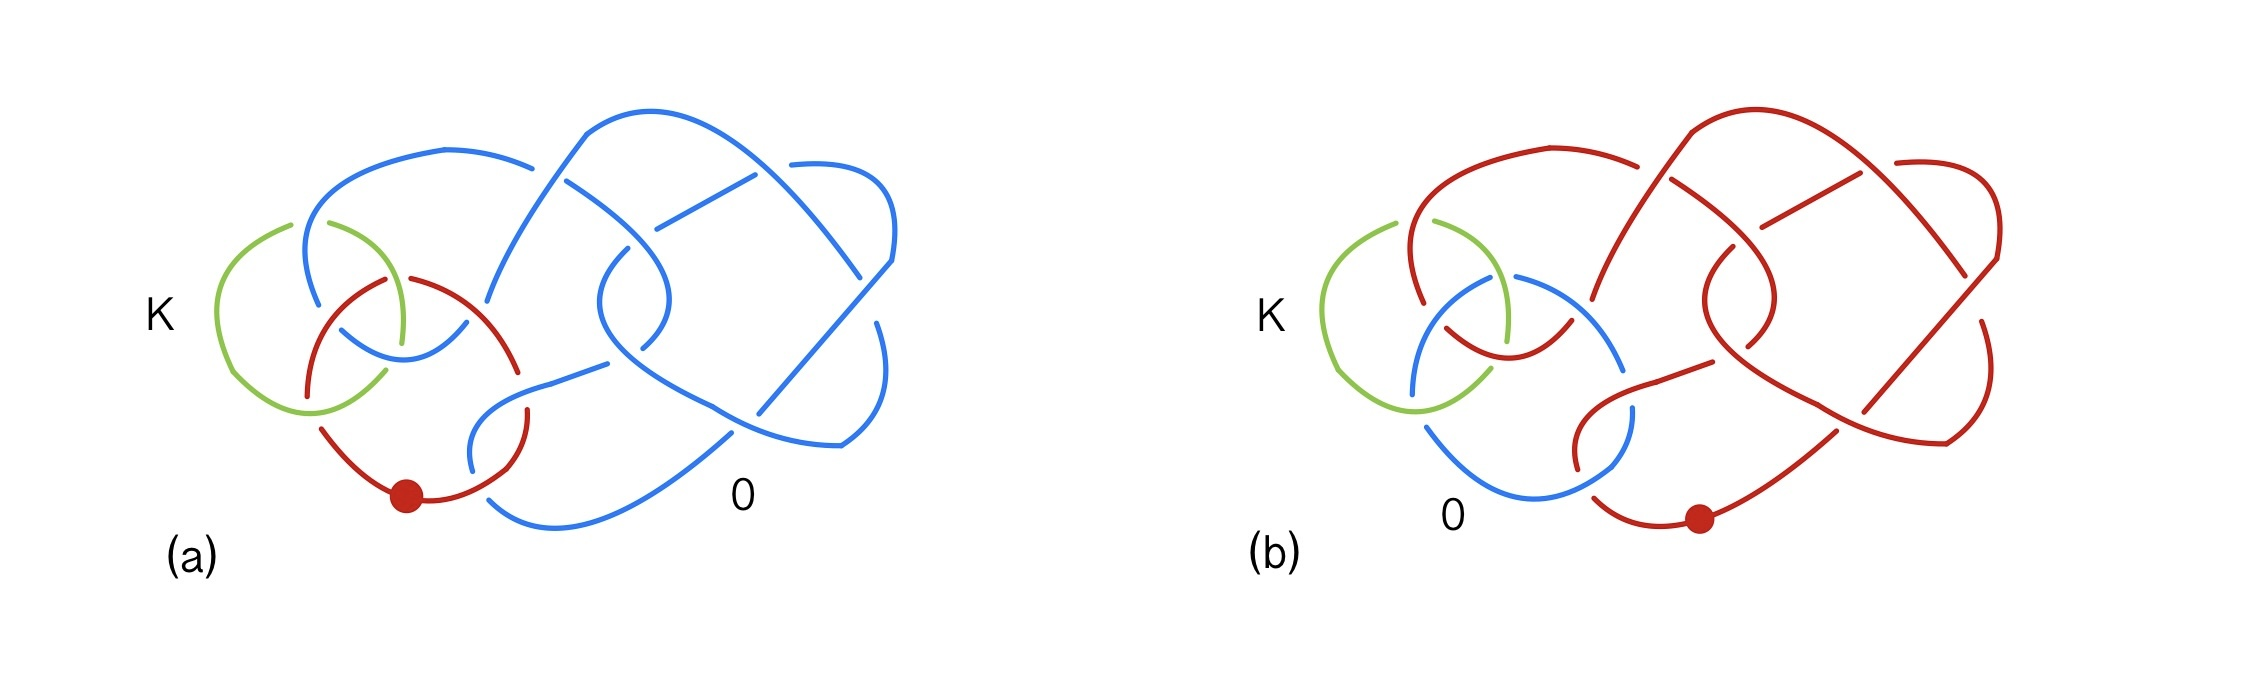
\includegraphics[scale=0.2]{figures/trecolori.jpeg}
    \caption{Two Kirby diagrams decorated with colors to enhance the roles of the handles}
    \label{fig:trecolori}
\end{figure}
\begin{obs}$\mathfrak{K}$ represents $\B^4$. 
\end{obs}
In fact, after a small isotopy, the core of the $1$-handle transversely intersects the cocore of the $2$ handle in one point. Therefore, we can perform a handle cancellation, that turns $D$ into the empty diagram. \\ \\
Let the third component of the quasi Brunnian link be $K$.
With this interpretation in mind, $K$ is a knot sitting inside $\partial \B^4 = \s^3$, presented with a non - standard surgery diagram. 
\begin{cla}$K$ bounds a slice disk, embedded in $\B^4$.
\end{cla}
The key point is that $K$ does not pass through the $1$-handle.
Clearly $K$ bounds a disk $D$ in $\s^3 \setminus A$. We then push the interior of $D$ in the interior of $\B^4 \cup (1-handle) = \s^1 \times \B^3$.
As a result, $D$ does not interfere with the attaching region of the $2$-handle.
Notice that this is possible because $A \cup K$ is split.
This procedure gives rise to the desired disk. \\ \\
Since the definition of quasi Brunnian link is symmetric (with respect to $A$ and $B$), we can swap the roles of $A$ and $B$. We place the red dot on $B$, and decorate $A$ with the $0$ label, as in Figure \ref{fig:trecolori}(b). Then we produce another disk $D'$ that bounds $K$ as before. We have created a pair of embedded slice disks which bound the same knot. 
From what has been said so far, it is not clear that such disks are ribbon.
This will become clear in the next section.
\section{Explicit Description of the Disks via Banded Unlink Diagrams}
The approach discussed above, is quite theoretical. As we will see, one can prove exoticness of the pair, in the topological setting, without any further description of $D$ and $D'$.
However, a bare hand approach may be mandatory to prove other properties of the disks. 
We start by redrawing $K$ in the standard surgery diagram of $\s^3$. At this point, we have a few options. \\ \\ In general, we can use the following algoritmic approach. We isotope $A \cup B$ to a Hopf link and we drag $K$ along such isotopy. Then, we perform multiple handle slides ($K$ over the $2$ handle), to unlink $K$ from the red circle. Then $K$ squishes through the blue circle. Now we can cancel the handle pair, and contemplate $K$ in the empty diagram of $\partial \B^4$. \\ \\
In some lucky cases, we can perform handle slides right away. It is the case of Figure \ref{fig:mag1}(a). After a small isotopy, we can immediately perform handle slides as in Figure \ref{fig:mag1}(c), (e). From (f) to (g) we use the light bulb trick to unlink $K$ from the $2$-handle, and then we cancel the handle pair (in the boundary). Figure \ref{fig:mag2}(h) depicts $K$ in the standard diagram of $\s^3$.
\begin{note} 
The boxed integer indicates a certain number of negative full twists. We will also allow half integers, meaning half twists. 
\begin{obs} \label{unico}
Since Kirby moves correspond to diffeomorphisms of $\B^4$ and since the mapping class group of $\s^3$ is trivial, every sequence of isotopies and Kirby moves leads to the same knot, up to isotopy.
\end{obs}
Roughly speaking, it is only a shift of perspective.
\end{note}
\begin{figure}[H]
    \centering
    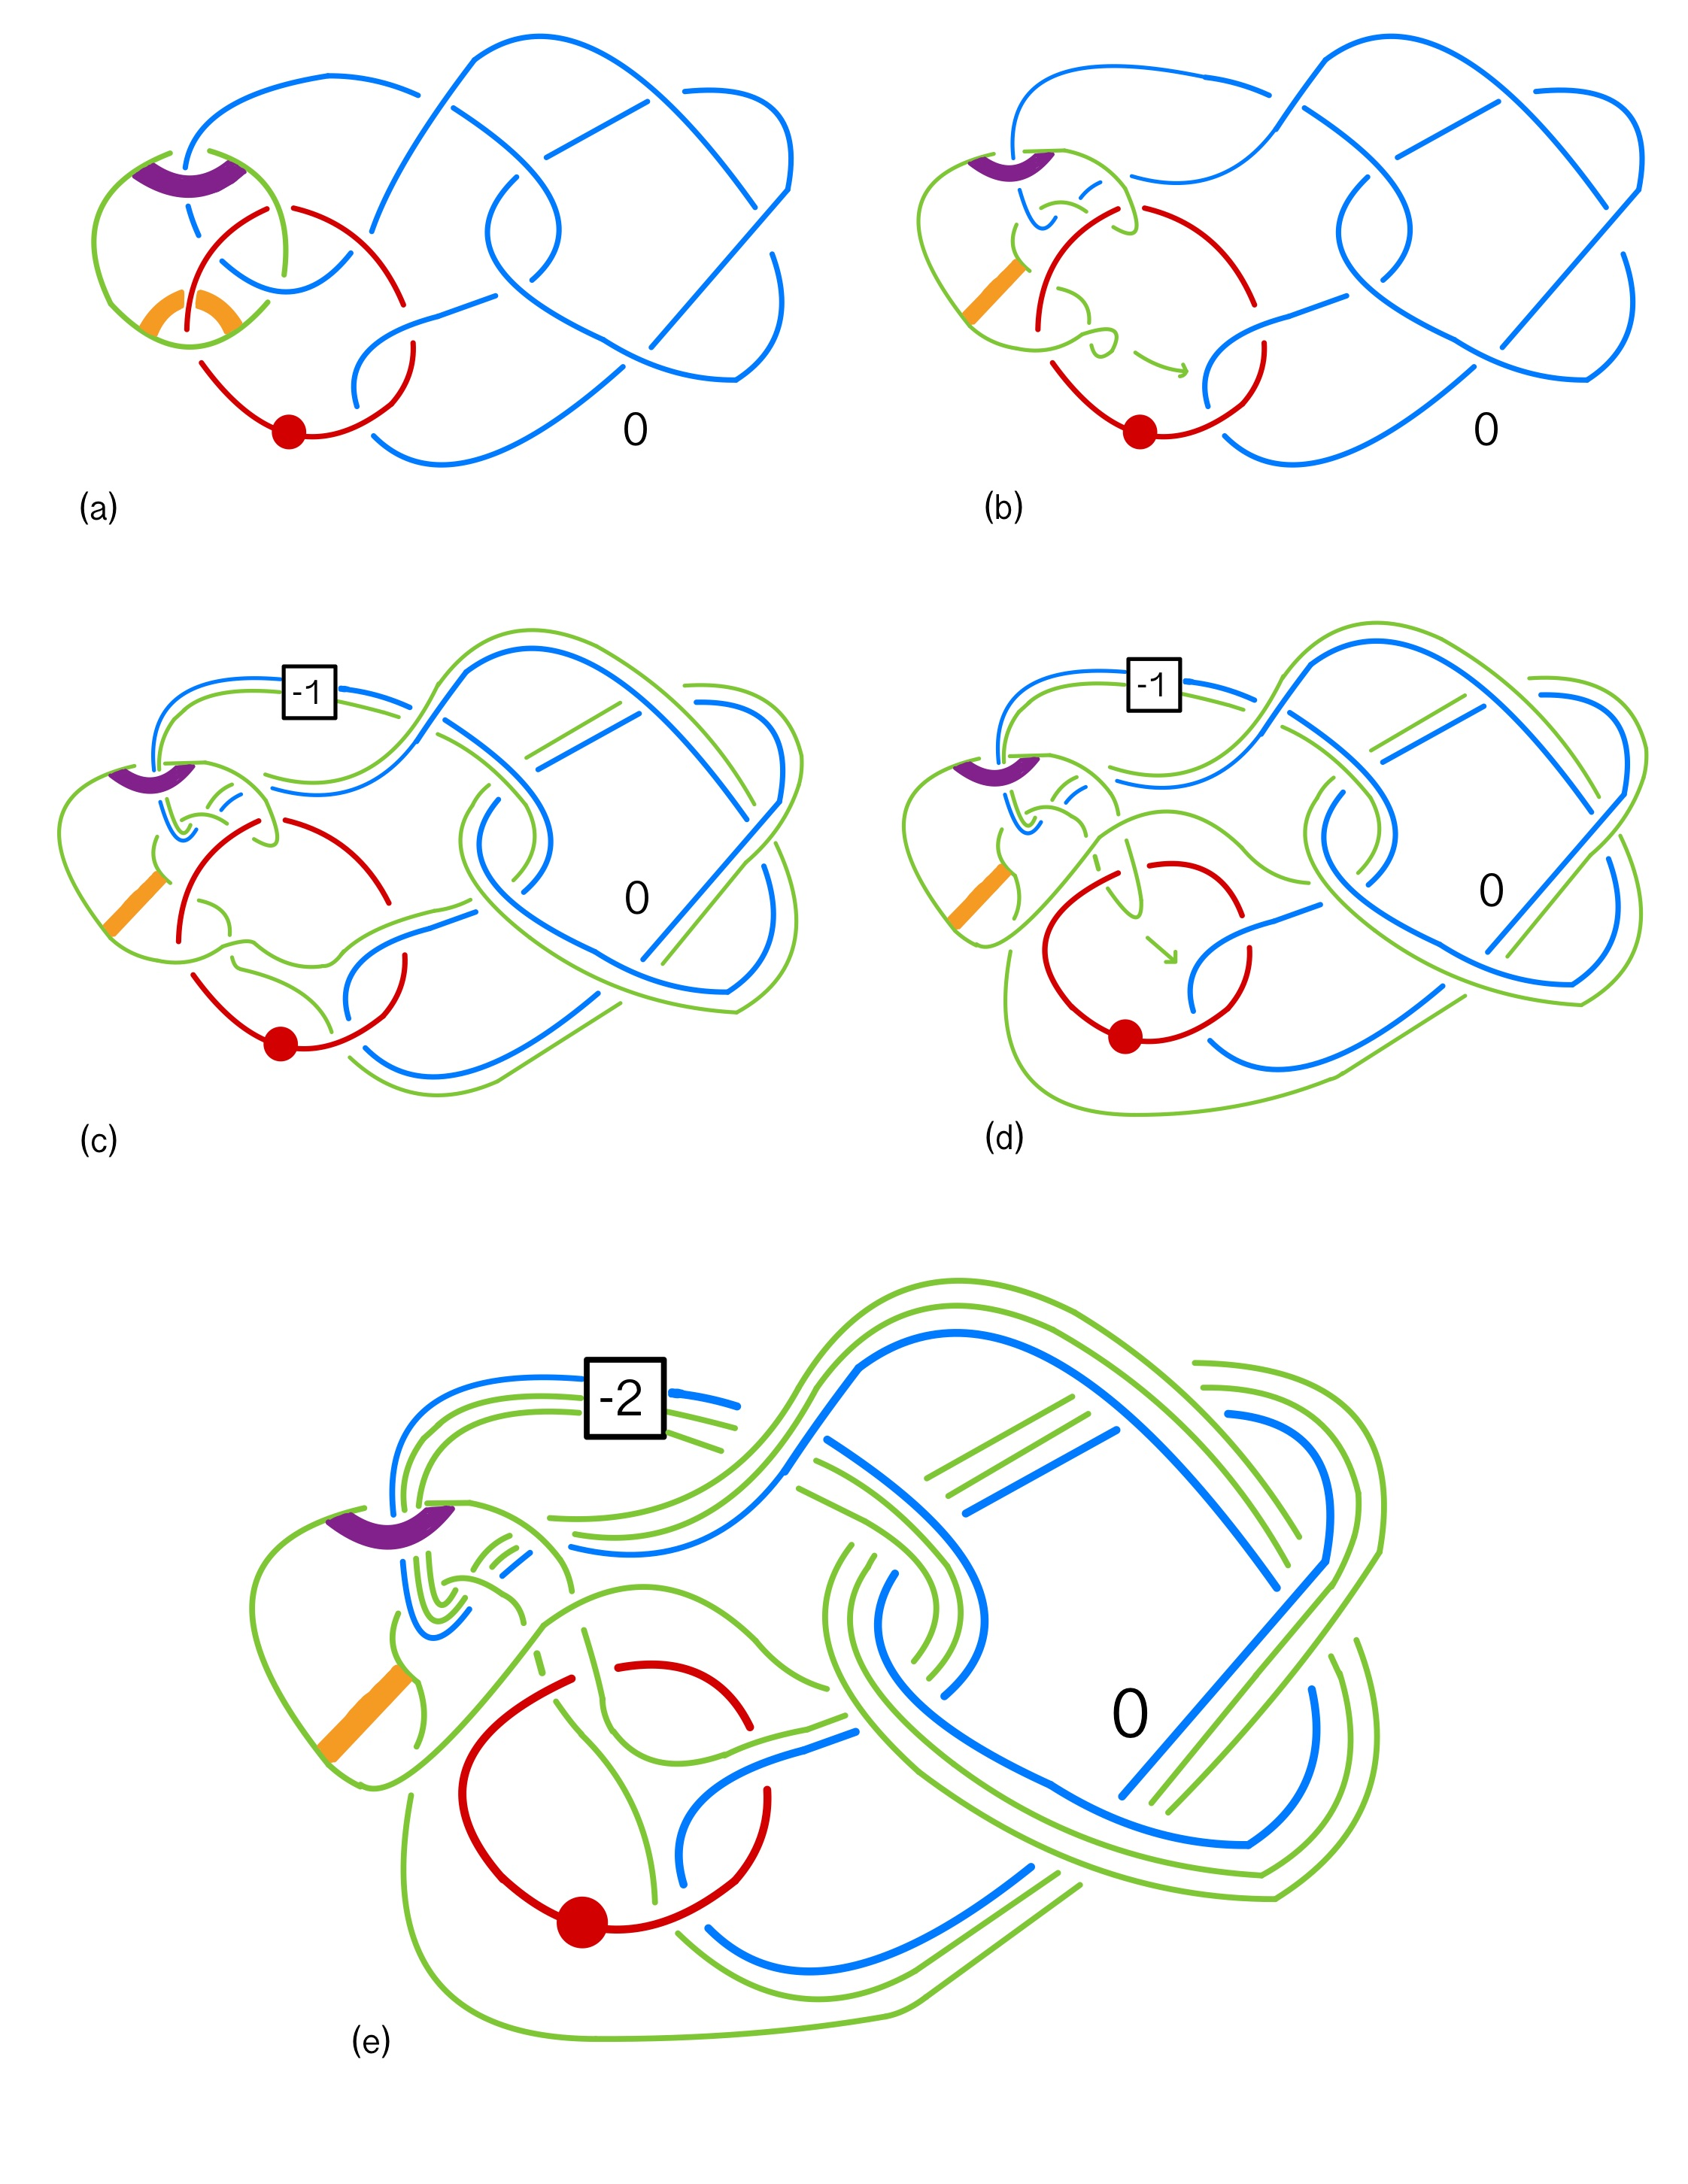
\includegraphics[scale=0.2]{figures/mag1.jpeg}
    \caption{A sequence of isotopies and Kirby moves}
    \label{fig:mag1}
\end{figure}
\begin{figure}[H]
    \centering
    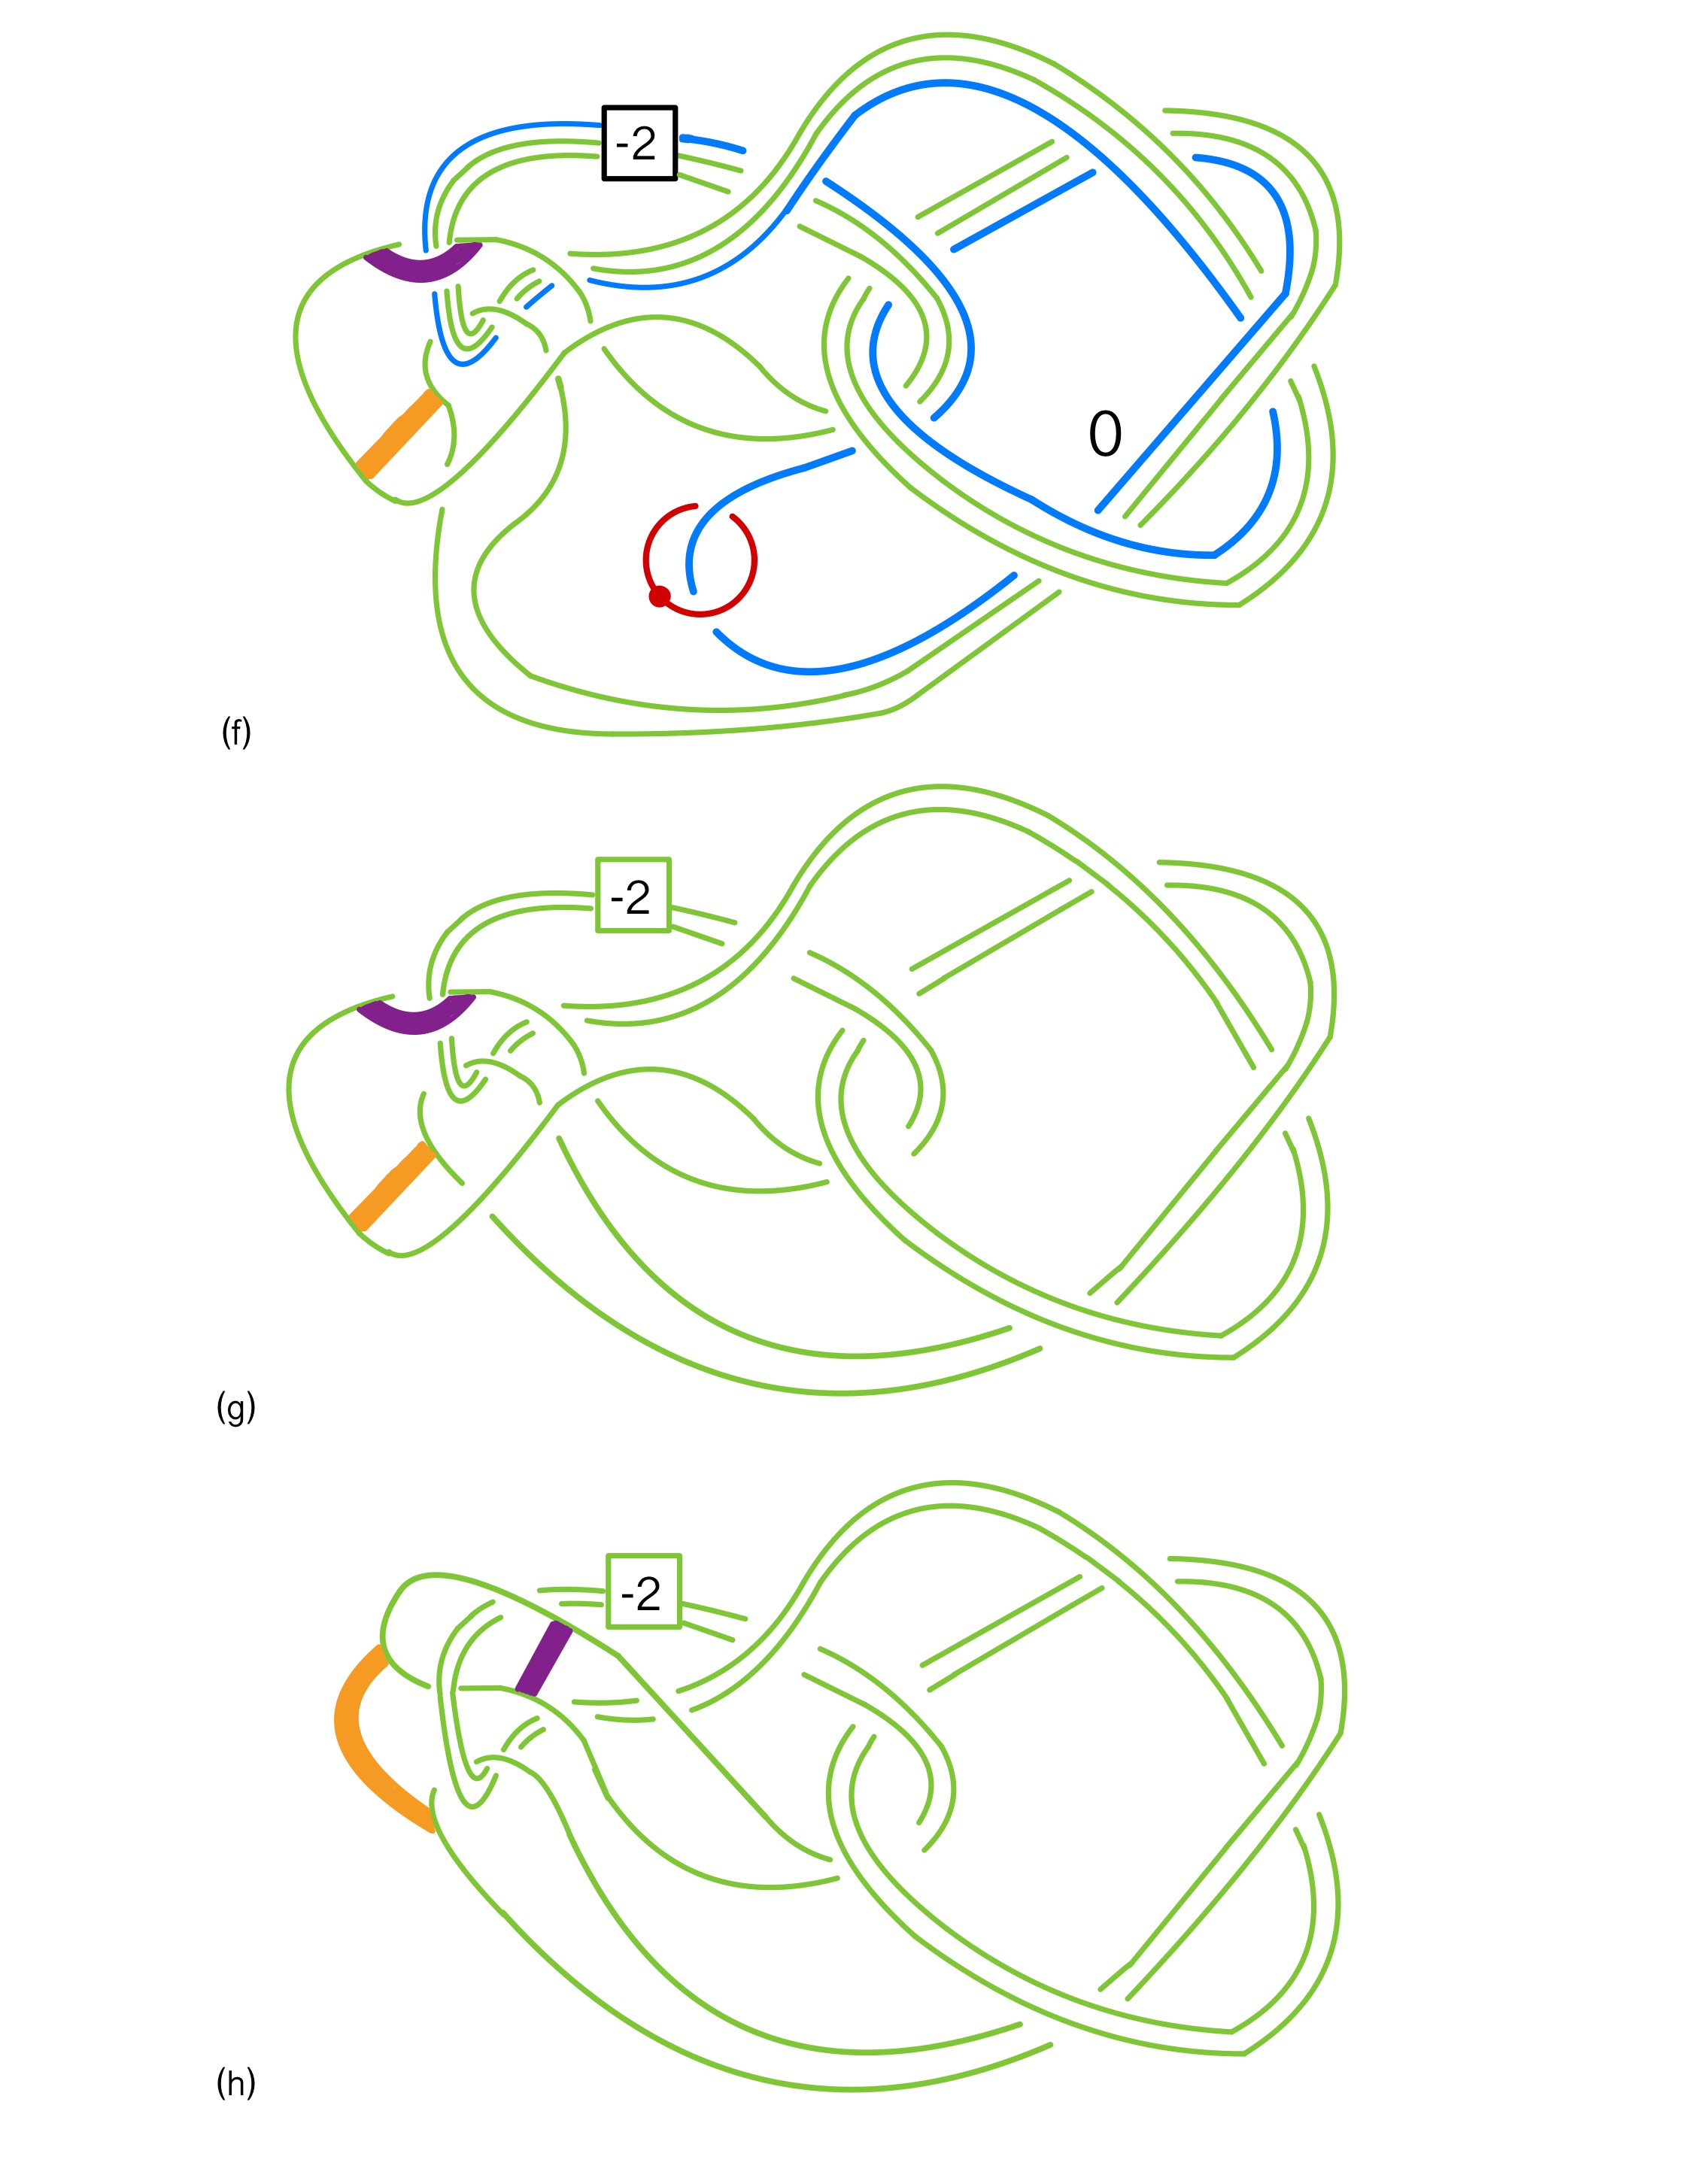
\includegraphics[scale=0.2]{figures/mag2.jpeg}
    \caption{A sequence of isotopies}
    \label{fig:mag2}
\end{figure}
In the previous figures, we kept track of two bands. 
\begin{as}The two bands, depicted in Figure \ref{fig:mag2}(h), define the disks $D$, $D'$ arising from the construction.
\end{as}
\proof
For background on banded unlink diagrams, we refer the reader to \cite{Hughes_2020}.
Consider the first picture \ref{fig:mag1}(a). 
The disk $D$ intersects the $2$-handle twice, resulting in two local minima in $\B^4$, which are cocores of the $2$-handle. The same is true for $D'$ after swapping the red with the blue circle2. Thus, there is only one ribbon band defining each disk \footnote{Each disk is almost described in the actual diagram where $K$ is a unknot}. Observe that band surgery on the orange band turns $K$ into two meridians for the red circle. On the other hand, band surgery on the purple band turns $K$ into two meridians for the blue circle. Thus, we identify the desired bands.
\endproof
It is now clear that $D$ and $D'$ are ribbon disks. \\
If we think about these bands, we can realize that they are pretty obvious.
Indeed, the purple band gives the natural ribbon structure, known as the "pair of glasses". On the other hand, the orange band joins the two minima disks of the previous structure. \\ \\
The latter example highlights the construction. Now we start proving the main theorem of this chapter. We repeat the same procedure to the following diagram.
\begin{figure}[H] 
    \centering 
    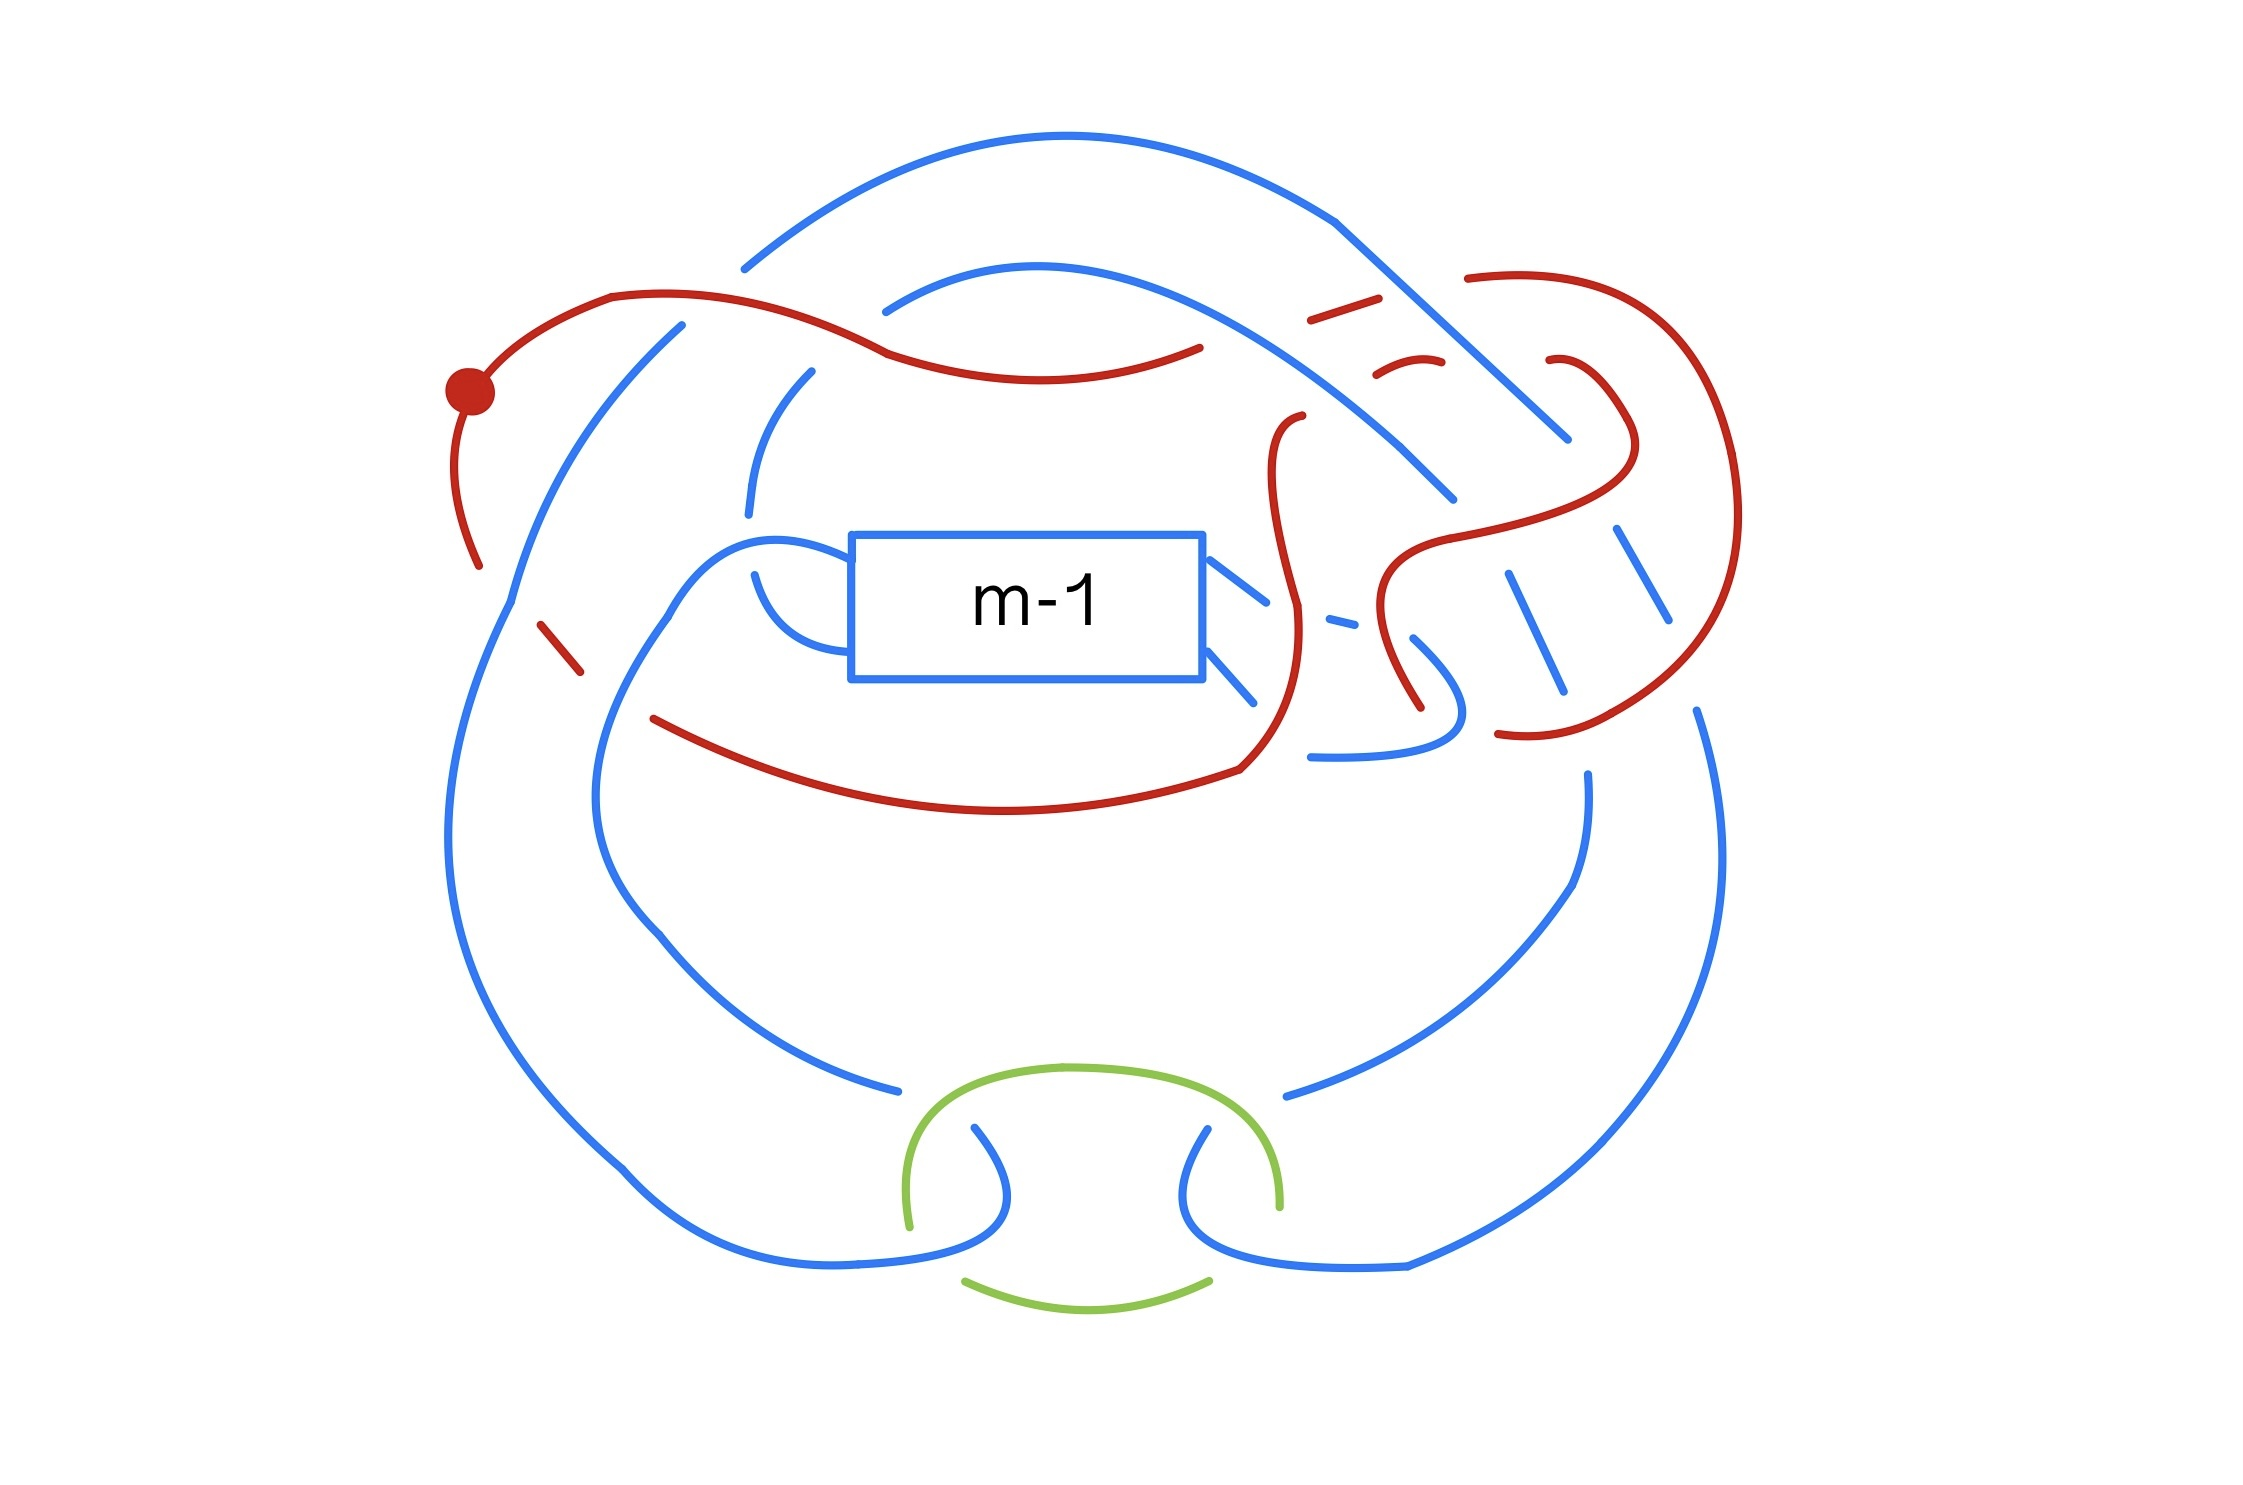
\includegraphics[scale=0.15]{figures/start.jpeg} 
    \caption{Another example of a quasi Brunnian link, labeled with colors} 
    \label{fig:start} 
\end{figure}
We call the green knot $K_m$.
We want to draw $K_m$ in the standard surgery diagram of $\s^3$. Moreover, we aim to find banded unlink diagrams of the disks $D$, $D'$ generated by Hayden's machine.
In this case we use the algoritmic approach: we turn the cancelling pair into a Hopf link. A sequence of isotopies is illustrated from Figure \ref{fig:triv1}(a) to Figure \ref{fig:triv4}(p).
\begin{figure}[H] 
    \centering 
    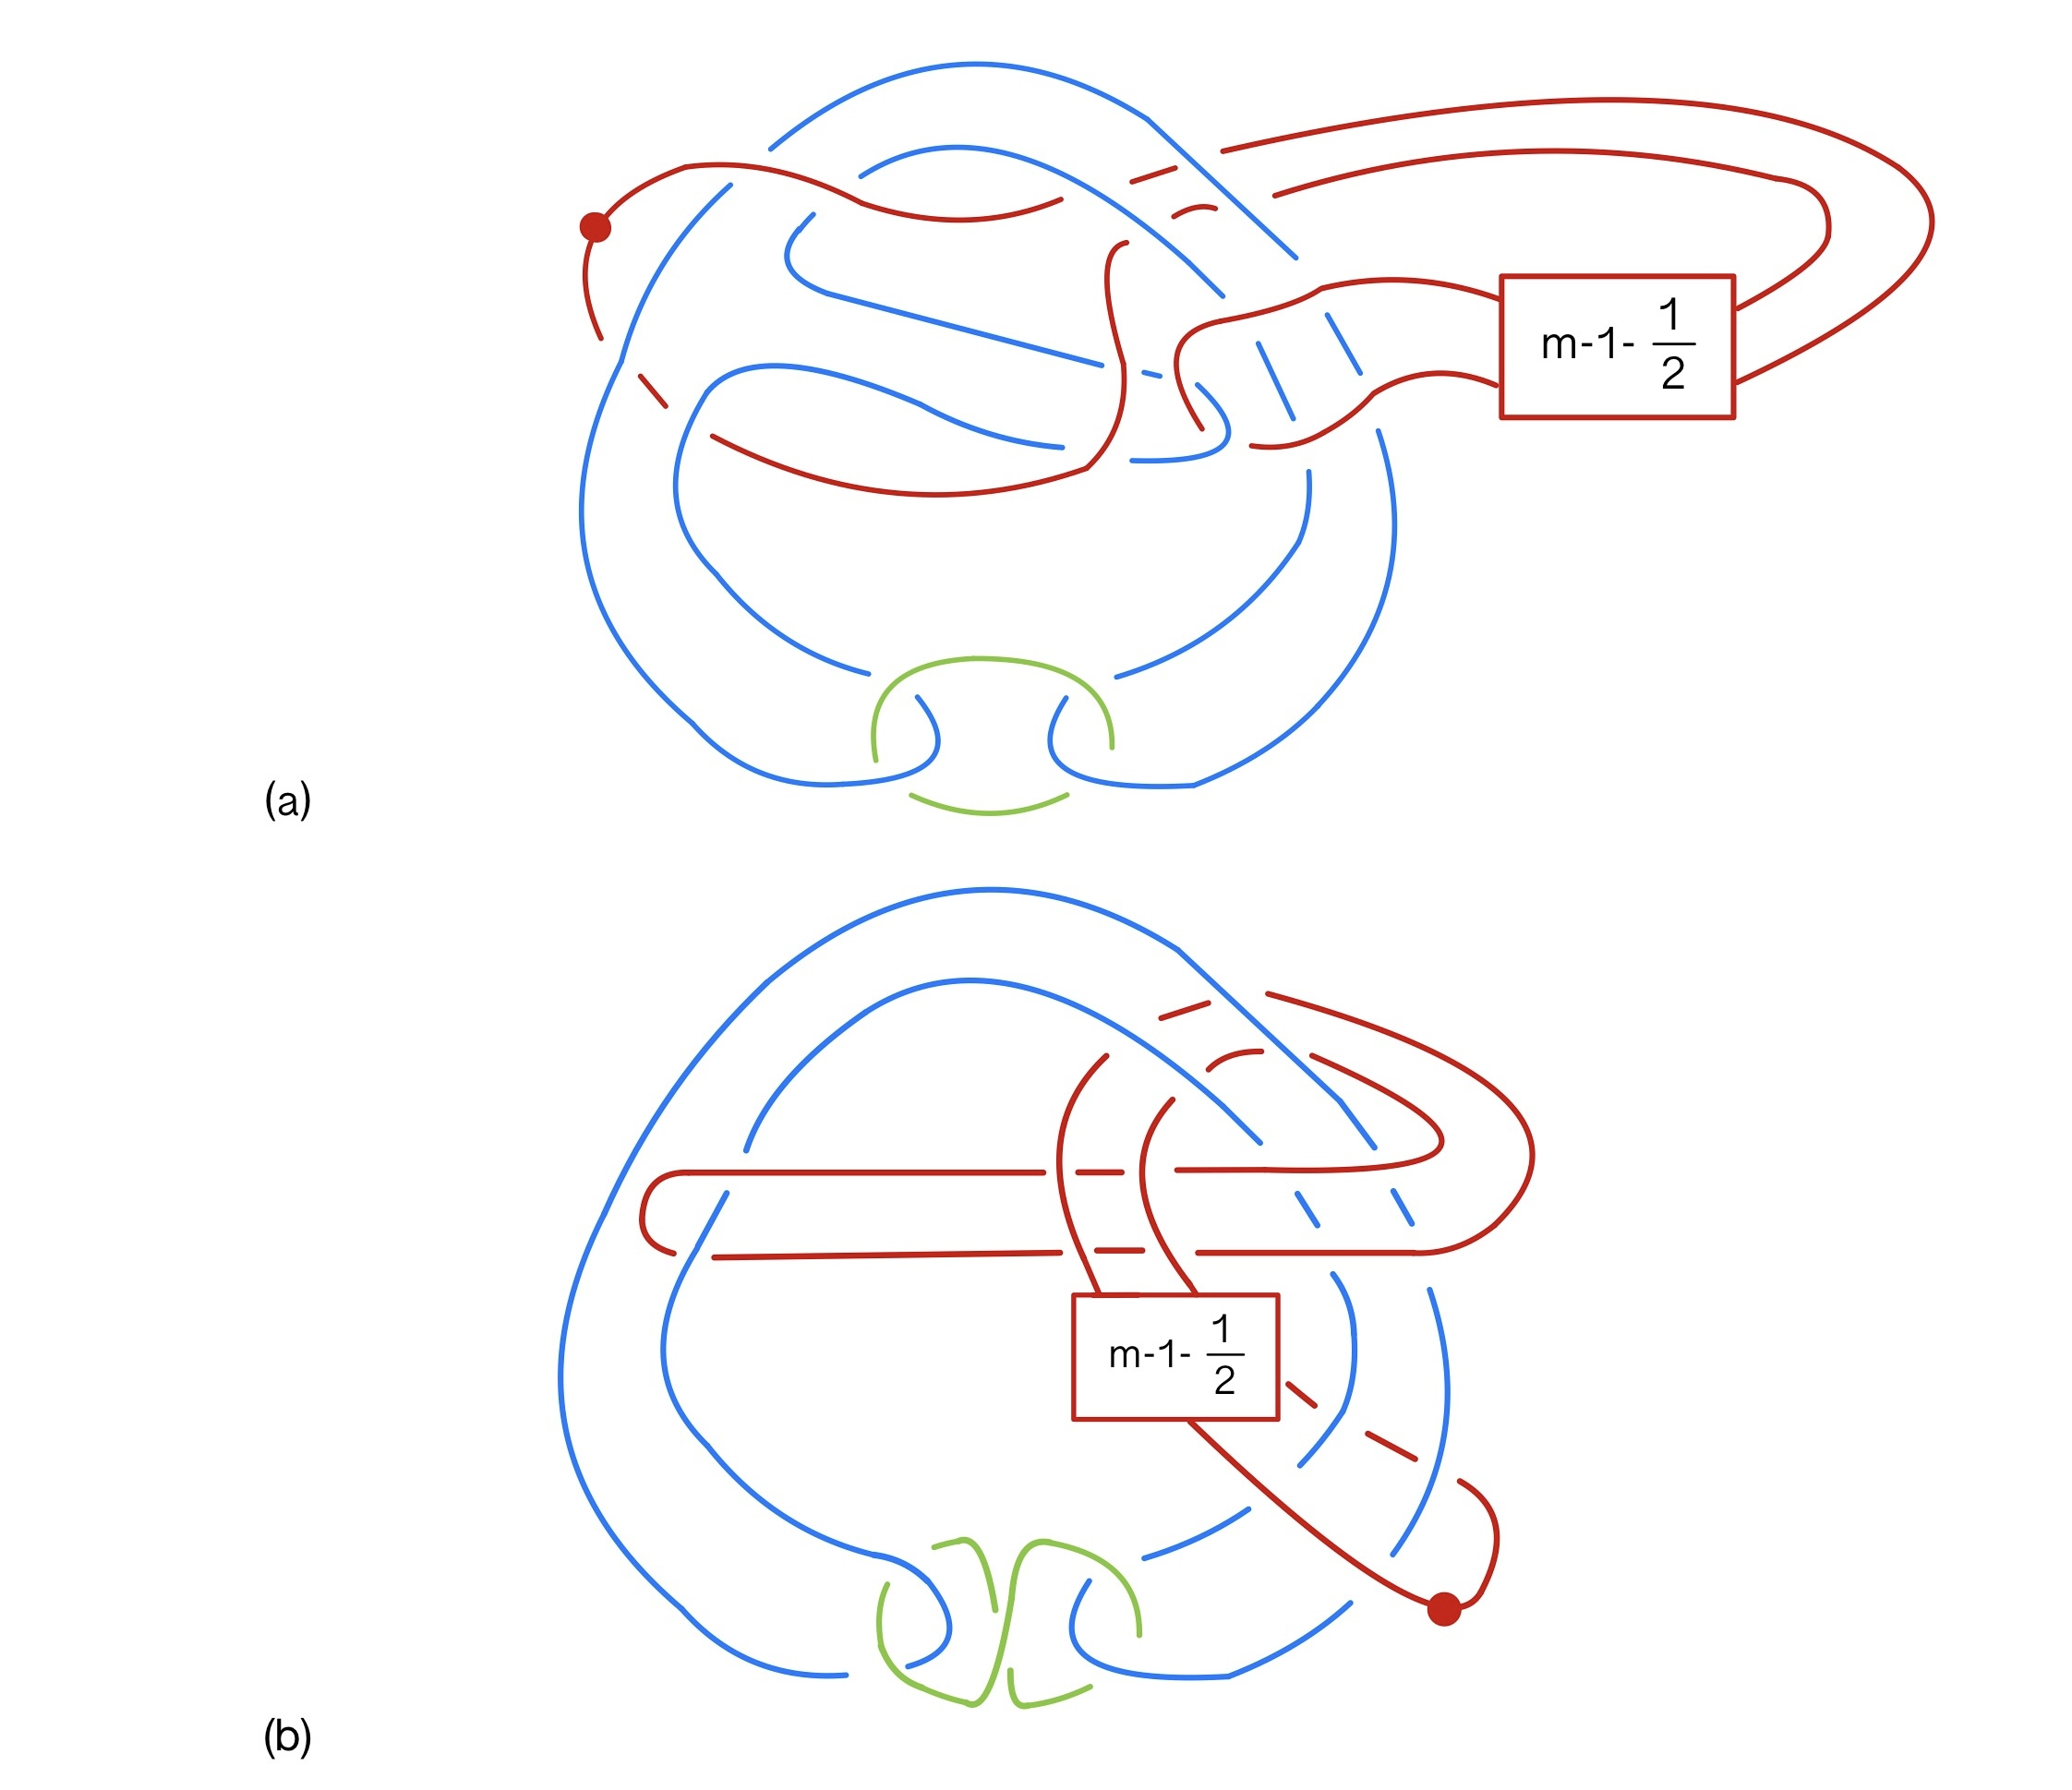
\includegraphics[scale=0.2]{figures/triv1.jpeg} 
    \caption{A sequence of isotopies} 
    \label{fig:triv1} 
\end{figure}
\begin{figure}[H] 
    \centering 
    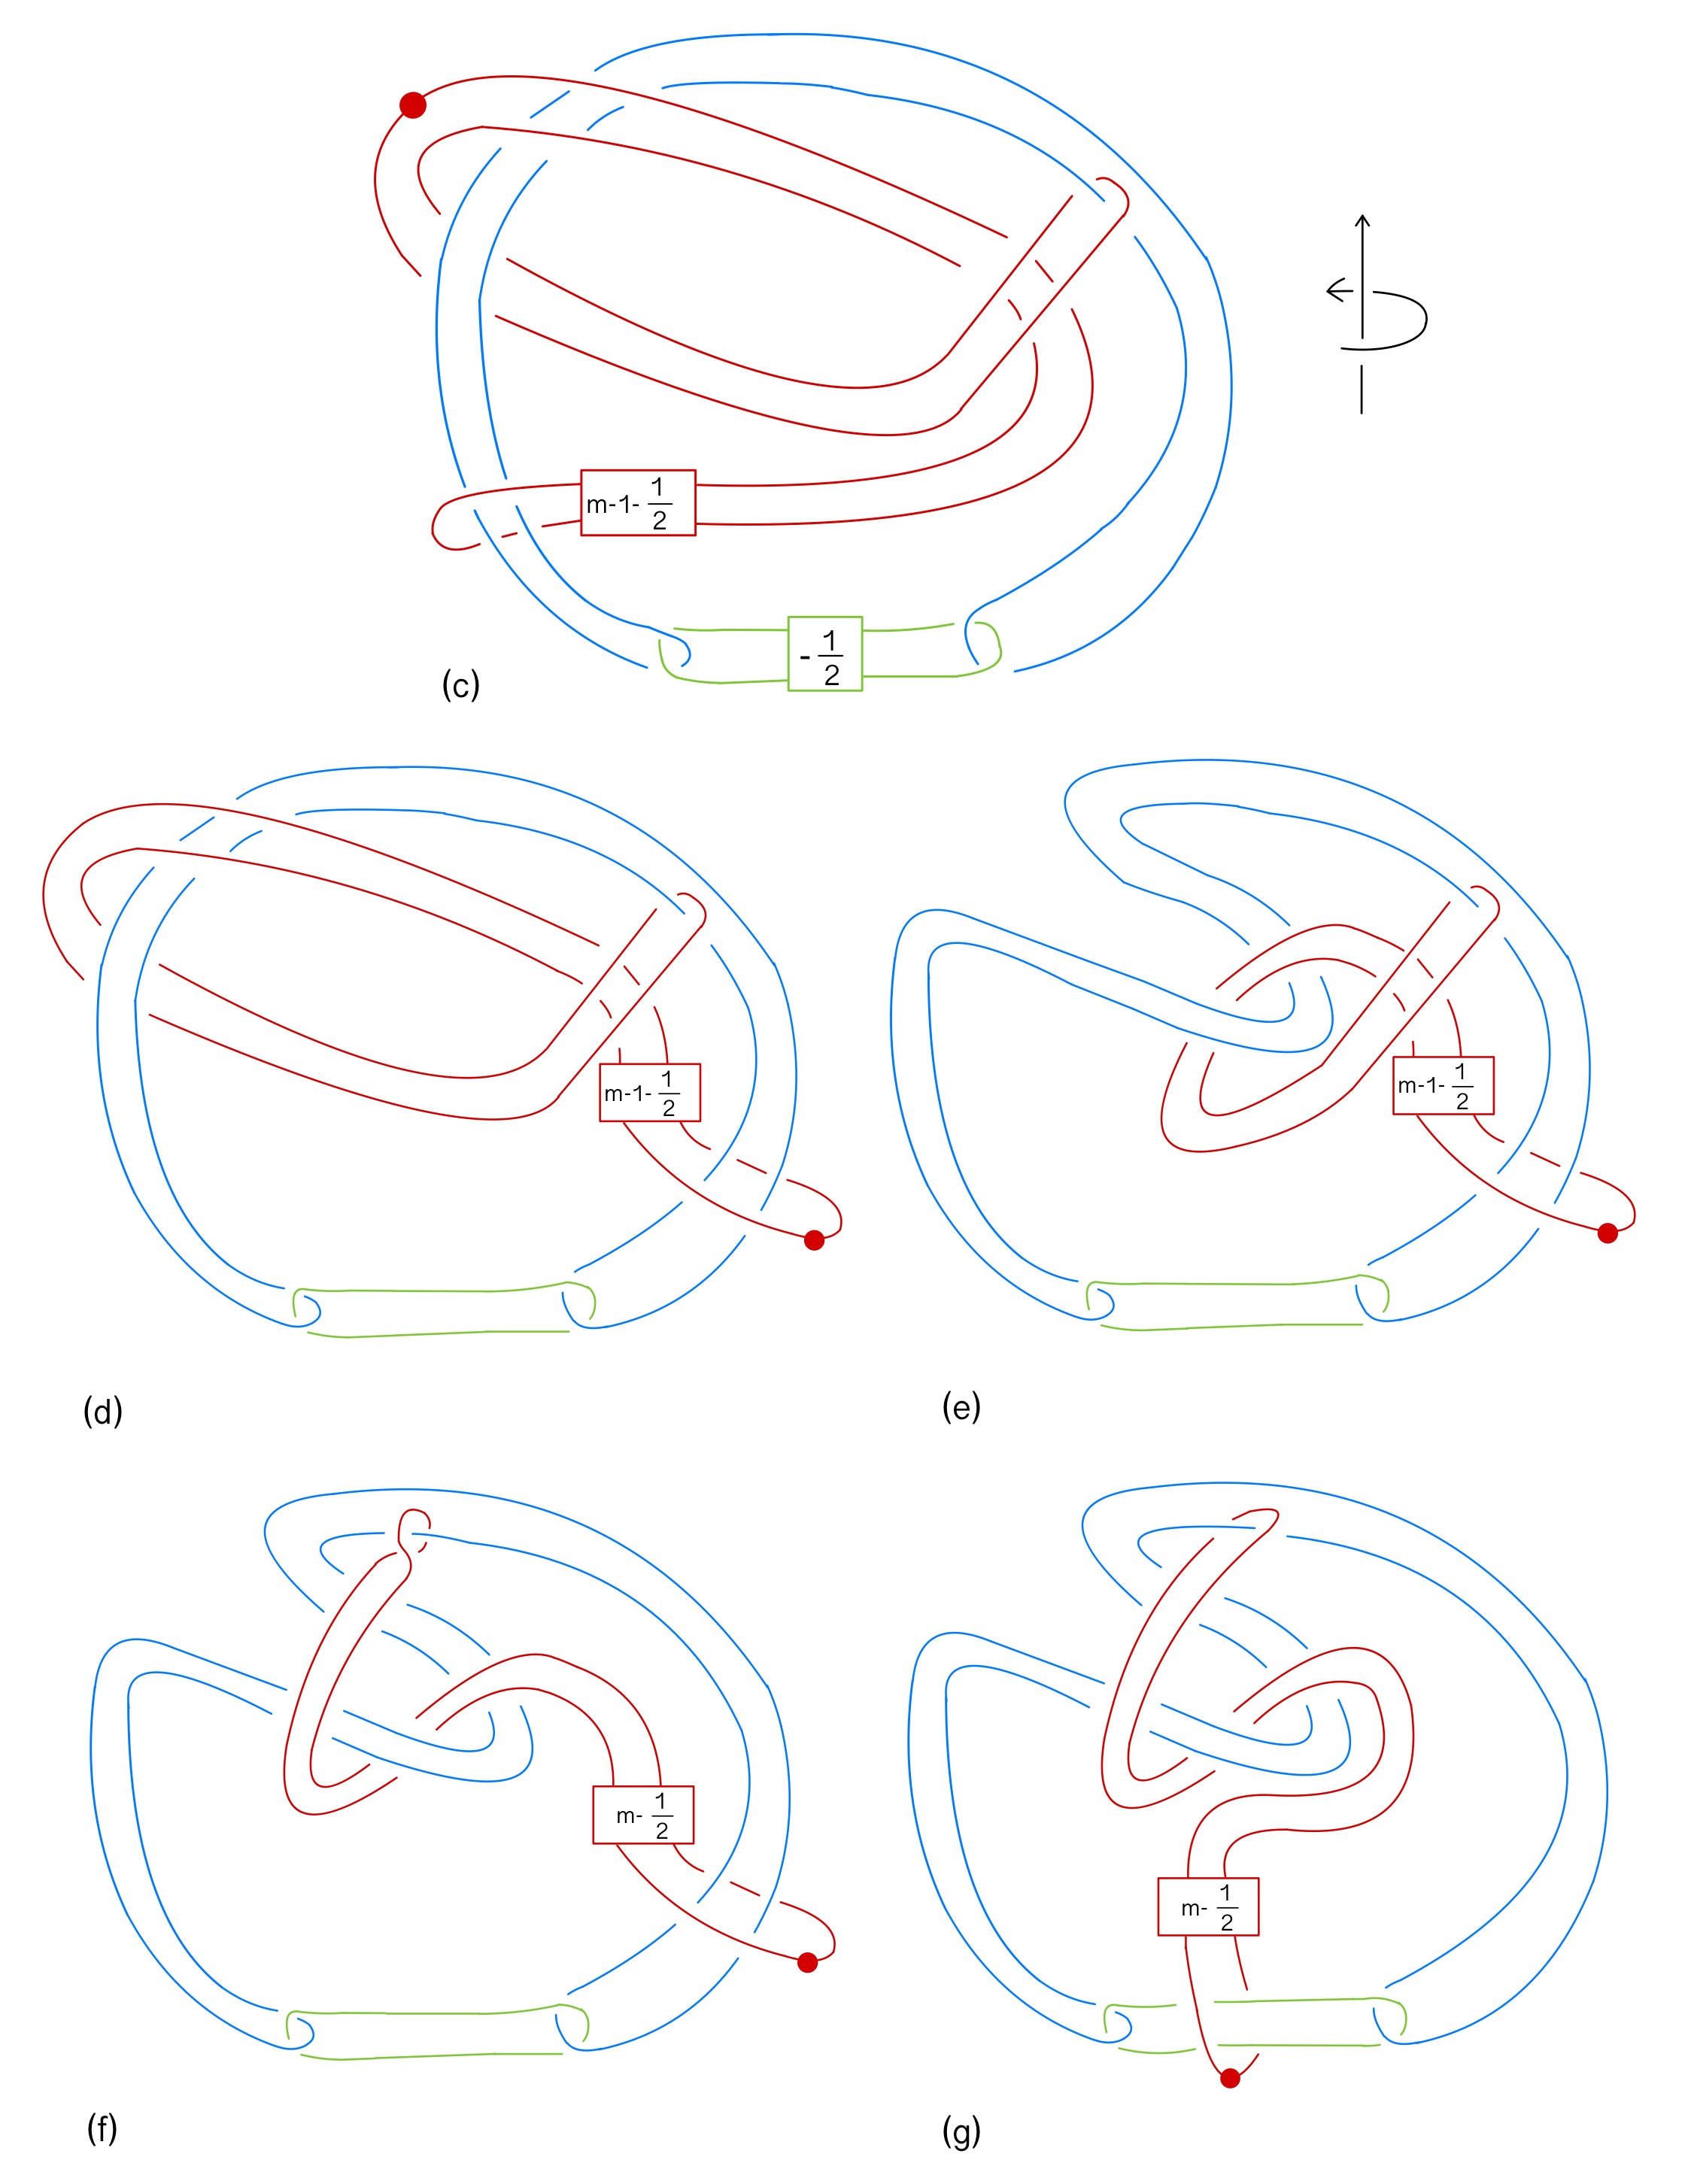
\includegraphics[scale=0.2]{figures/triv2.jpeg} 
    \caption{A sequence of isotopies} 
    \label{fig:triv2} 
\end{figure}
\begin{figure}[H] 
    \centering 
    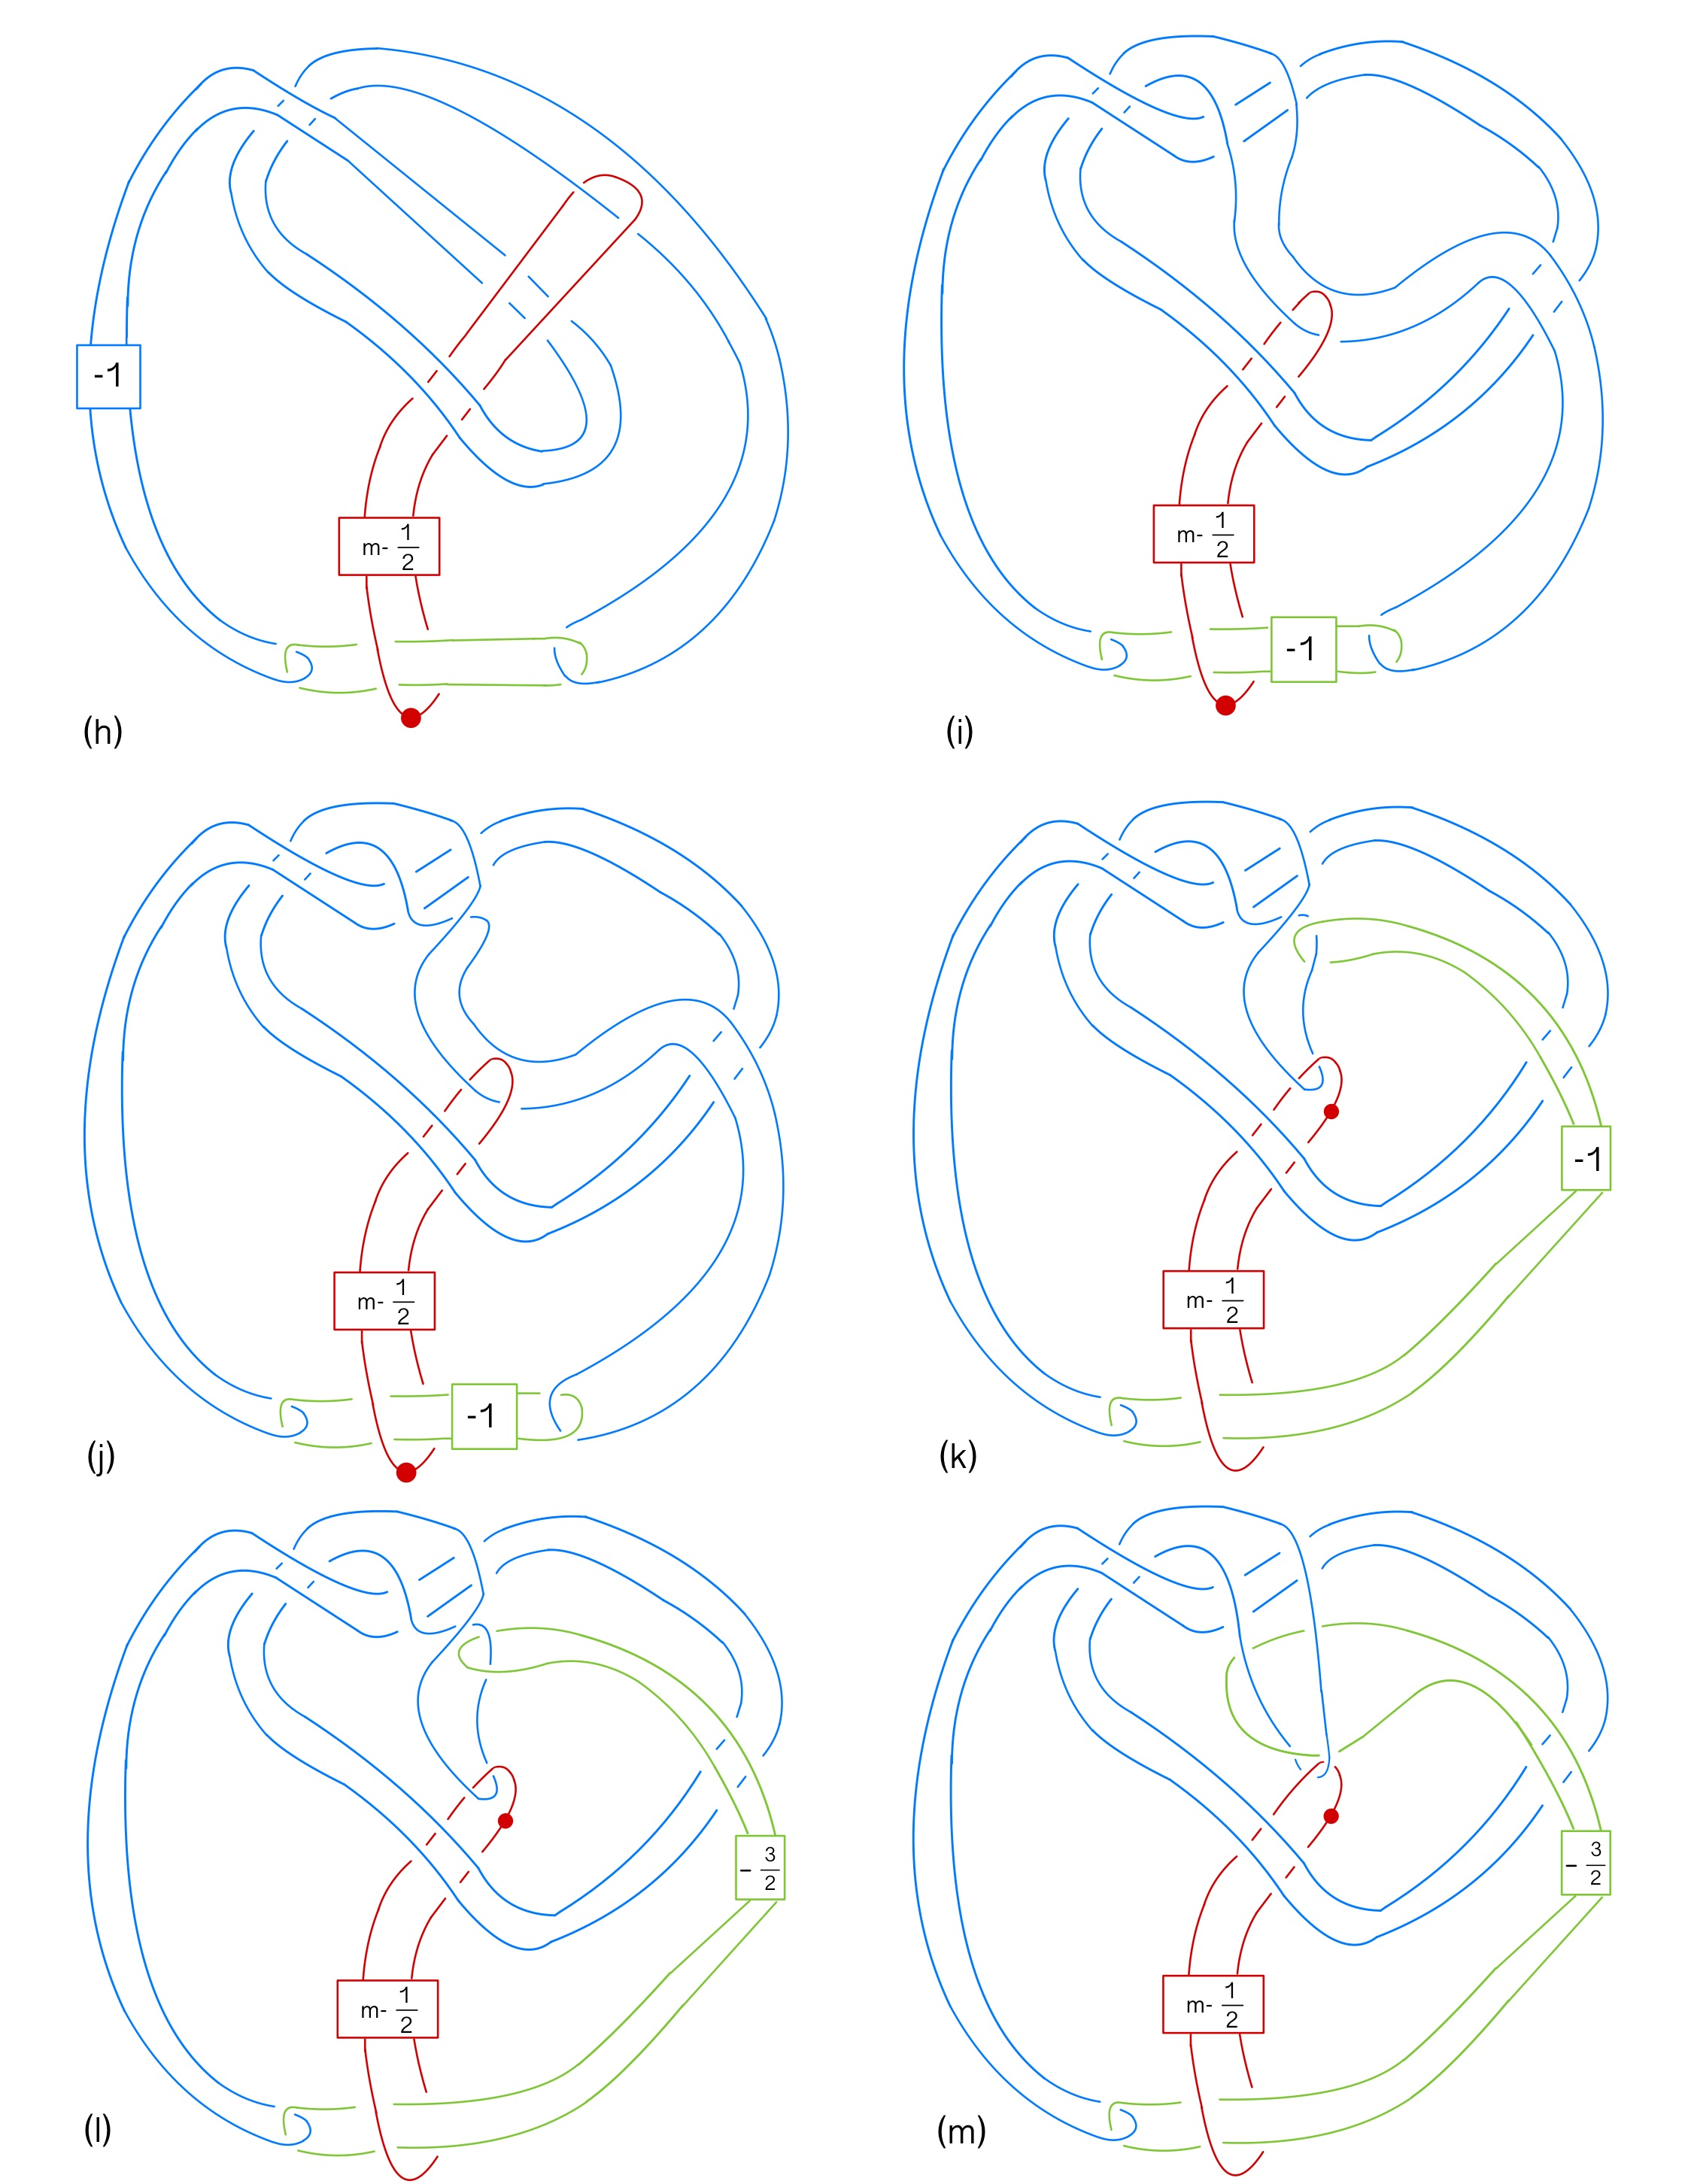
\includegraphics[scale=0.2]{figures/triv3.jpeg} 
    \caption{A sequence of isotopies} 
    \label{fig:triv3} 
\end{figure}
\begin{figure}[H] 
    \centering 
    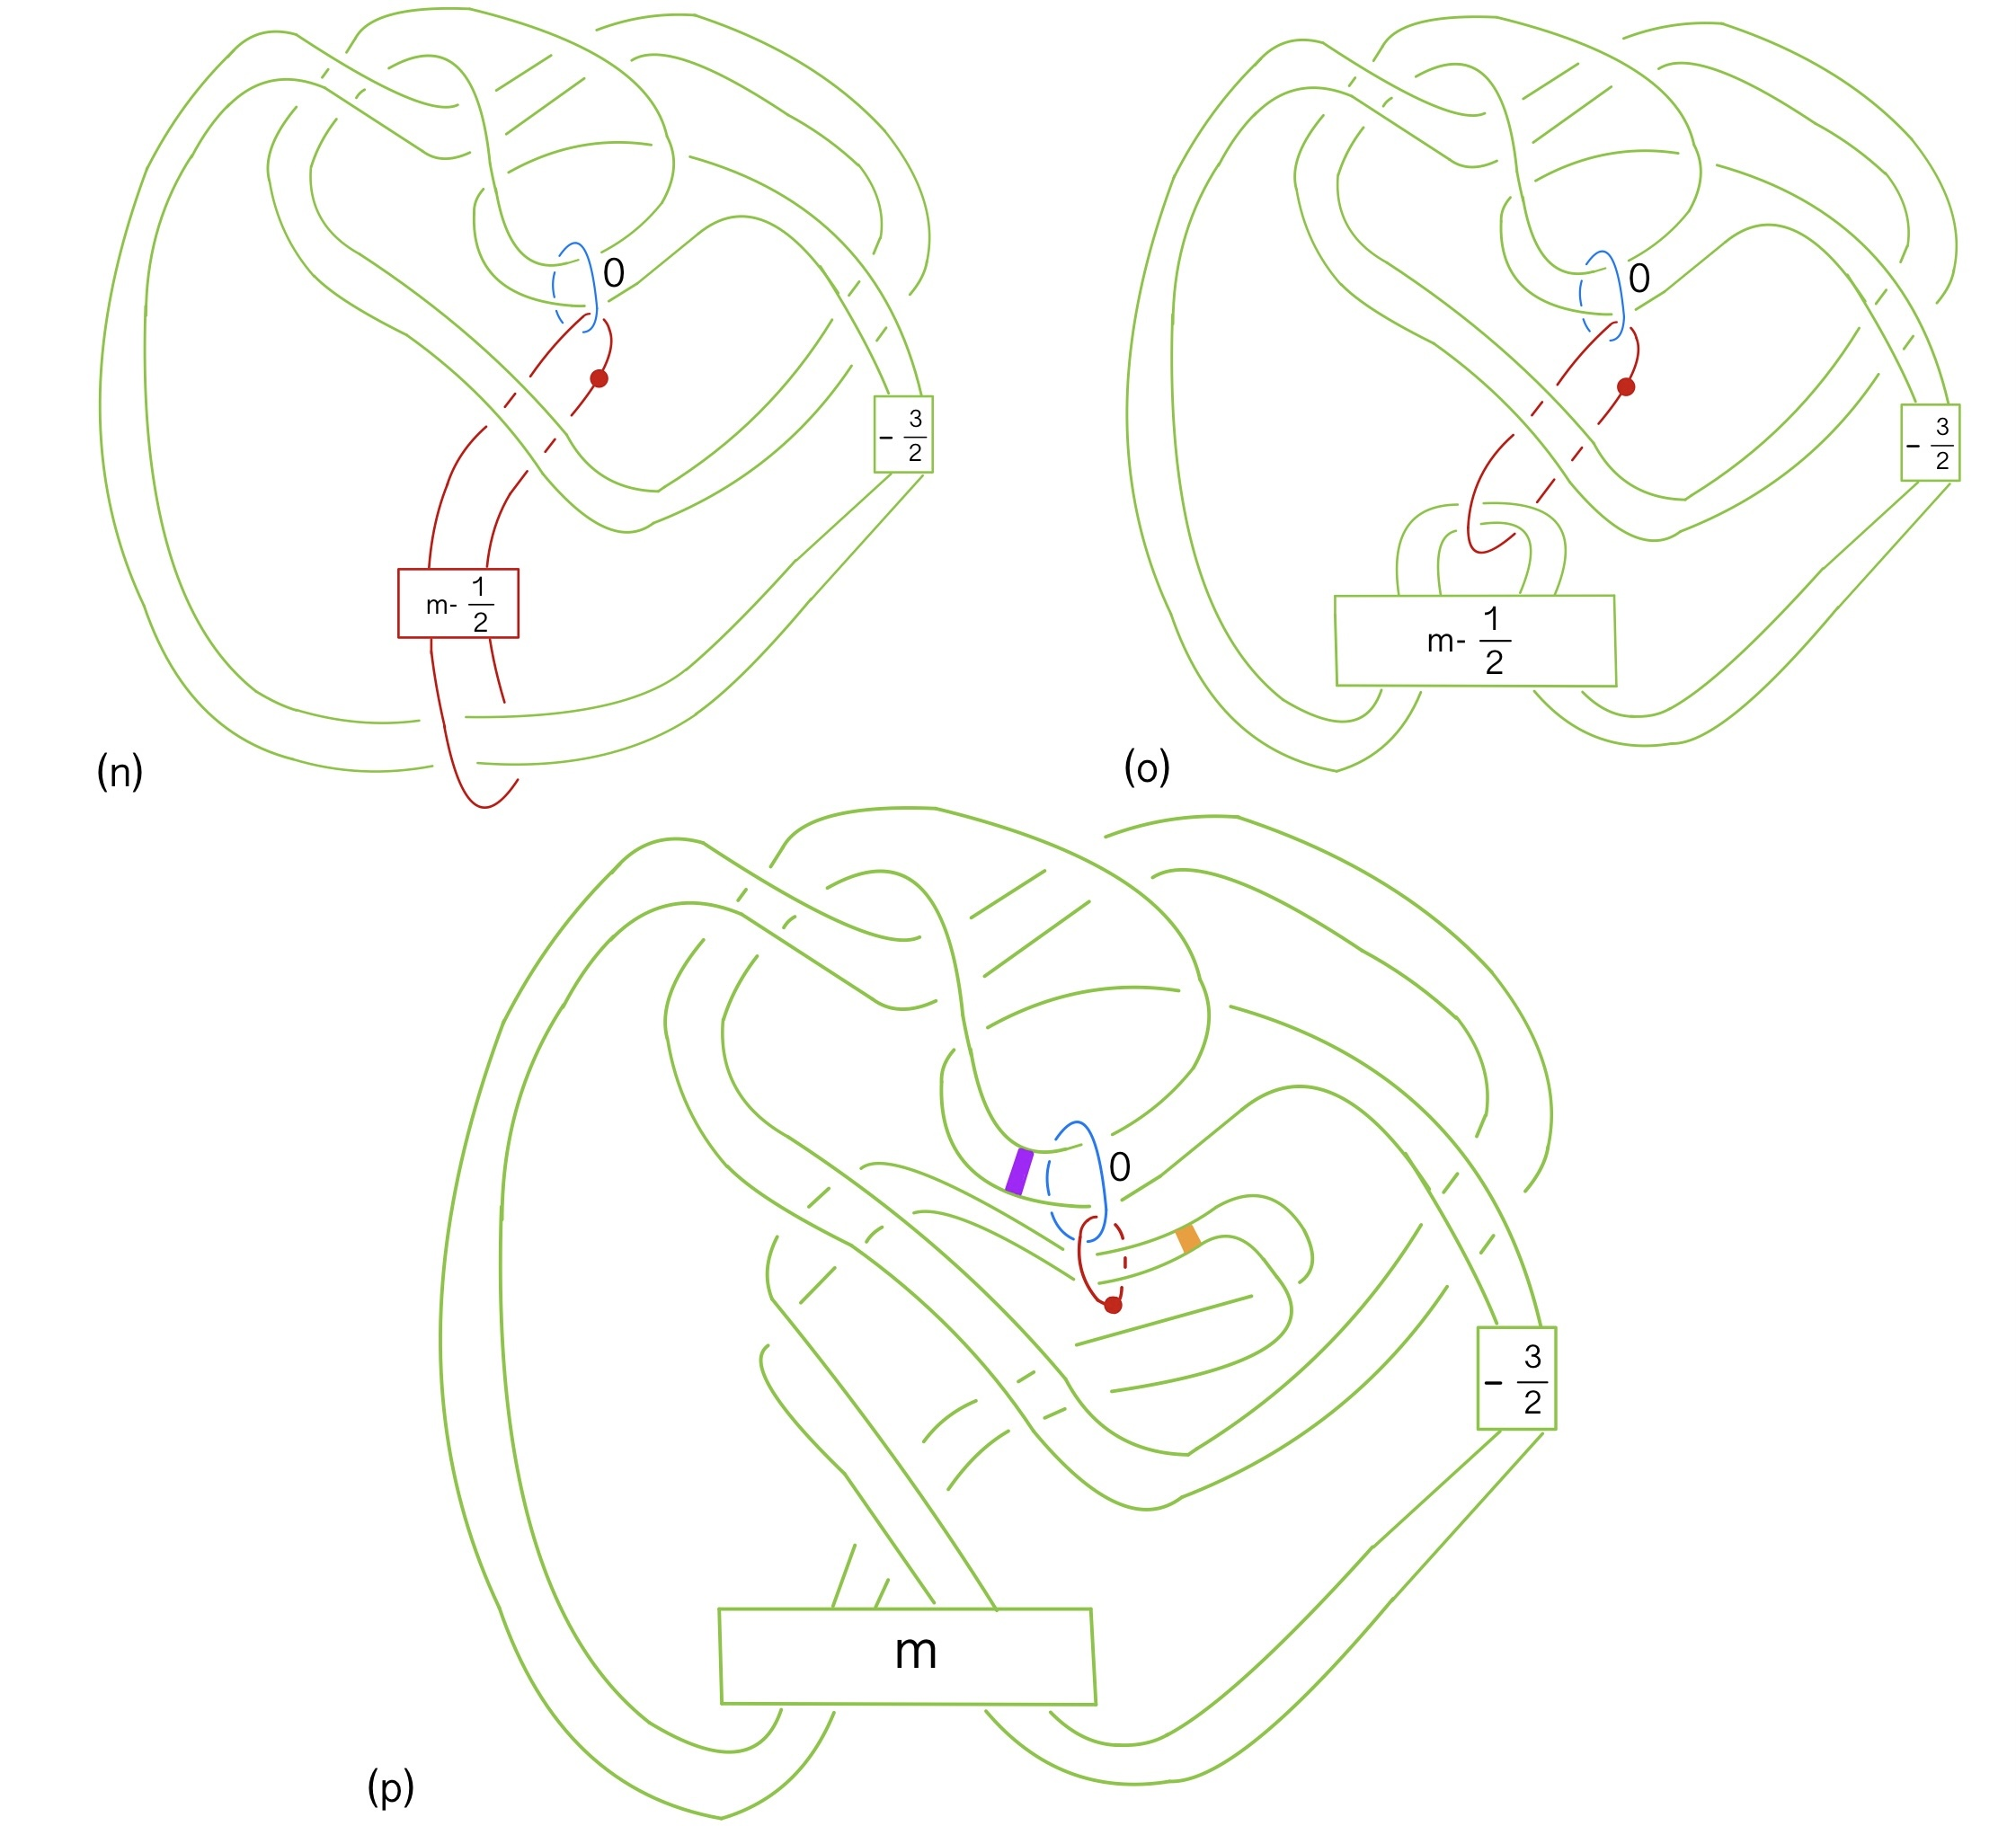
\includegraphics[scale=0.2]{figures/triv4.jpeg} 
    \caption{A sequence of isotopies} 
    \label{fig:triv4} 
\end{figure}
From now on, we track the two bands depicted in Figure \ref{fig:triv4}(p).
As in the first example, $D$ and $D'$ both have one saddle and two minima.
Notice that orange band surgery turns $K_m$ into two meridians for the blue circle. On the other hand, purple band surgery turns $K_m$ into two meridians for the red circle \ref{app} (that will be the $2$-handle after the exchange). \\
In Figure \ref{fig:triv5}(a)-(d), we slide $K_m$ two times over the $2$ handle. We include only some fragments for clarity. Figure \ref{fig:triv5}(e) shows the whole picture after the slides.
\begin{figure}[H] 
    \centering 
    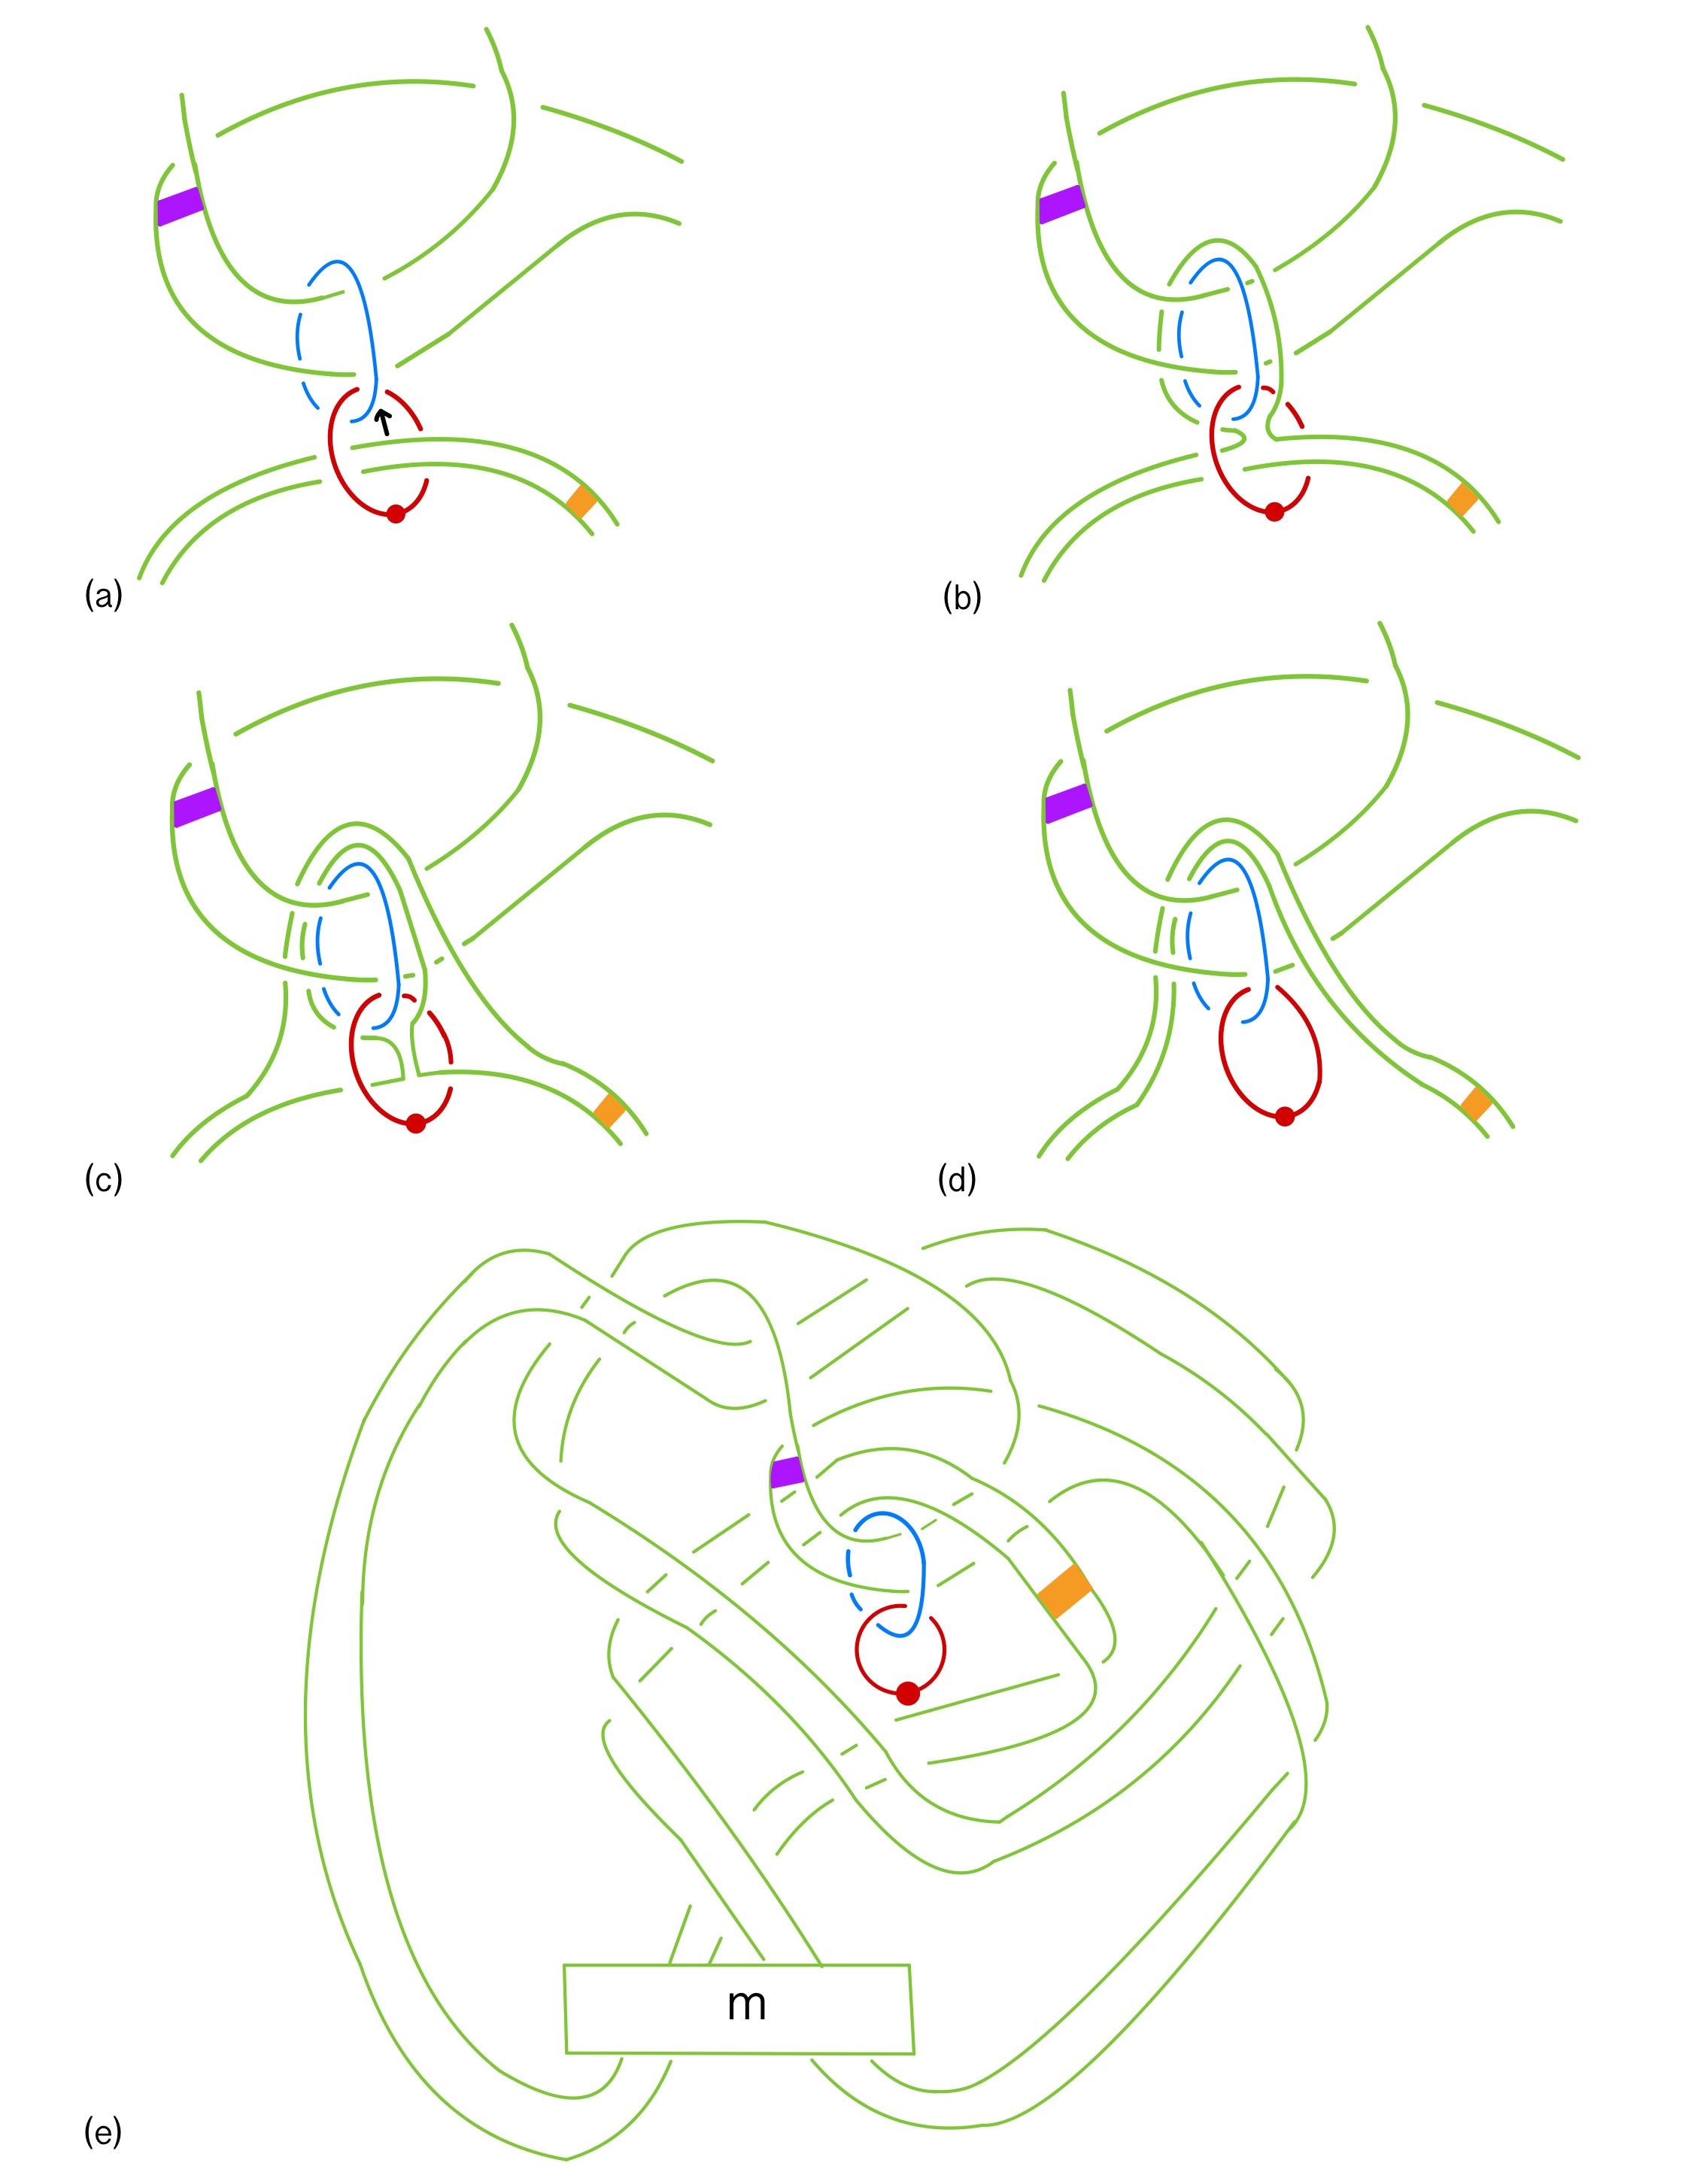
\includegraphics[scale=0.2]{figures/triv5.jpeg} 
    \caption{Handle slides} 
    \label{fig:triv5} 
\end{figure}
Finally, we cancel the handle pair. Figure \ref{fig:km} shows $K_m$ sitting inside the standard diagram of $\s^3$. It is decorated with an orange band and a purple band, which define $D$ and $D'$, respectively. We also depict a knot $J$ in the exterior of $K_m$, which will be used later on.
\begin{figure}[H]
    \centering
    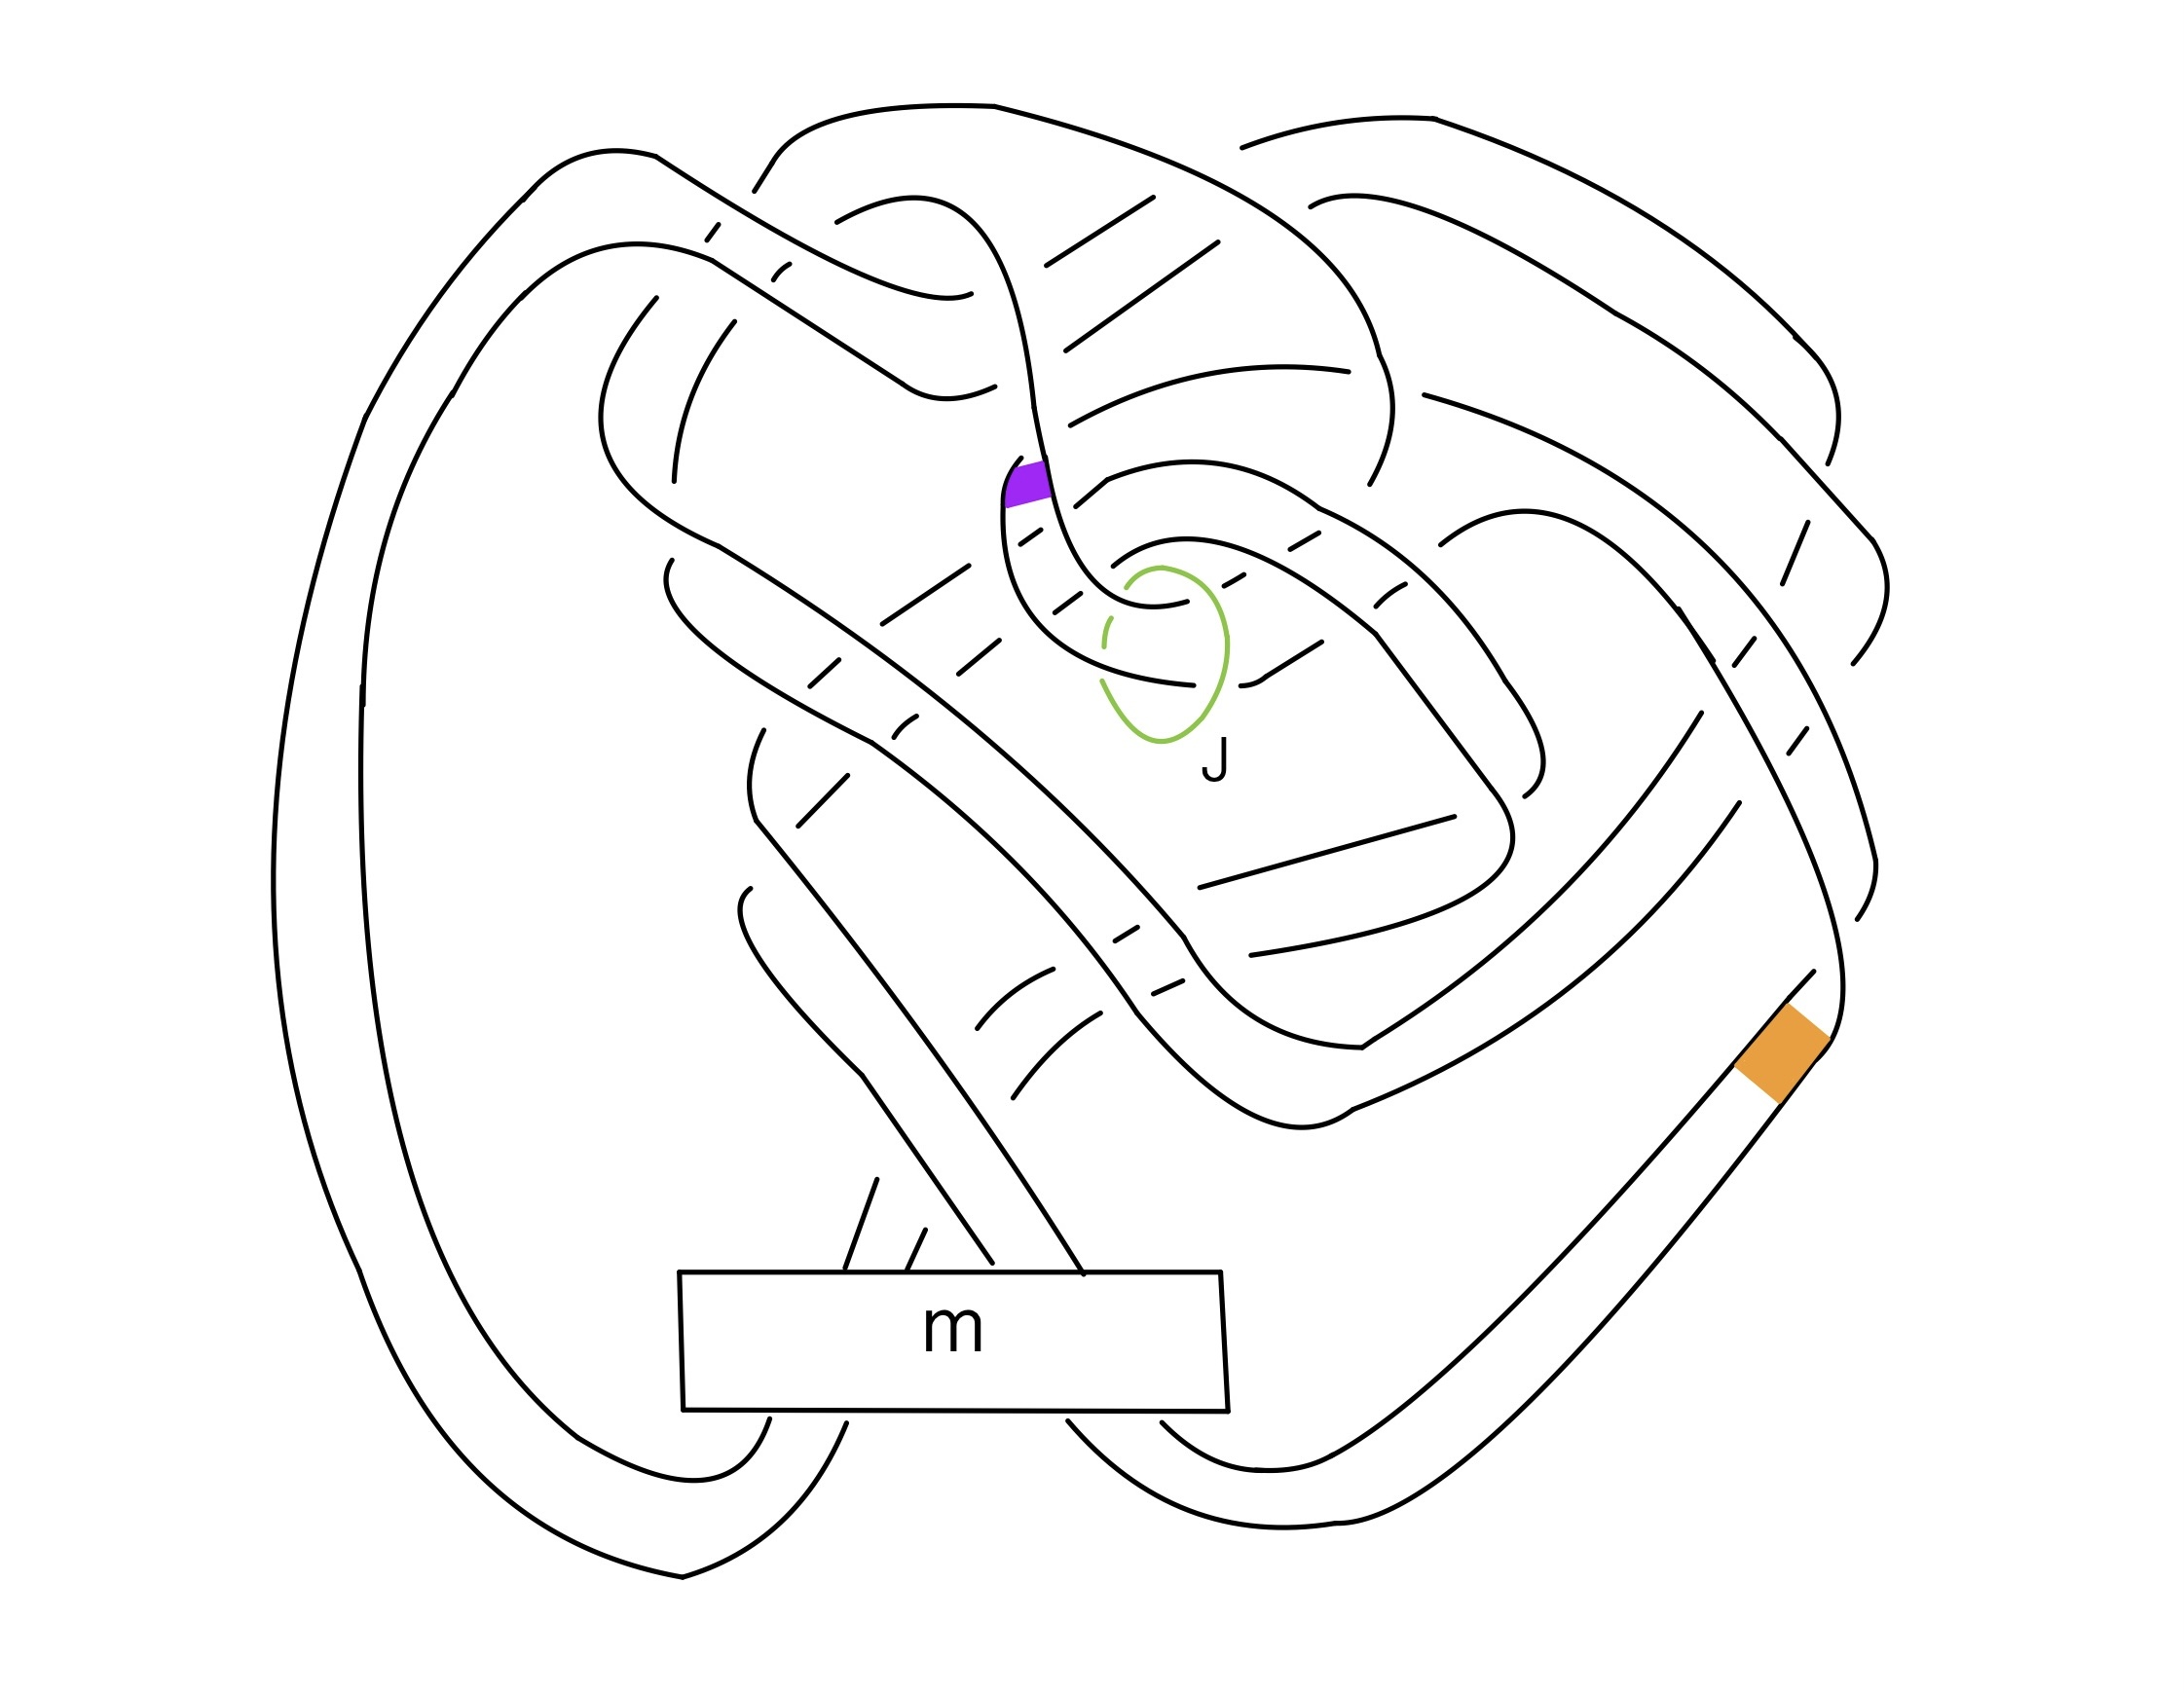
\includegraphics[scale=0.2]{figures/km.jpeg}
    \caption{The knot $K_m$ in $\s^3$, with two bands corresponding to the ribbon structure of $D$ and $D'$}
    \label{fig:km}
\end{figure}
The proof of Theorem \ref{prince} is divided into three steps. \\
(A) $D$ and $D'$ are smoothly isotopic to symplectic disks, \\
(B) $D, D'$ are topologically isotopic, \\
(C) $D, D'$ are not smoothly isotopic. \\ 
\newpage
\textbf{Proof of A} \\
Our goal is to construct a positively transverse link movie\footnote{For background, we refer the reader to \cite{lickorish1997introduction}, \cite{geiges2008contact}} to apply the following Lemma.
\begin{lem}\label{cob}Let $S \subseteq\B^4$ be a properly embedded surface, presented by a sequence of transverse links in $(\s^3, \xi_{st})$ related by the moves depicted in Figure \ref{fig:moves} and transverse isotopy. Then $S$ is smoothly isotopic ,relatively to the boundary, to a symplectic surface in $(\B^4, \omega_{st})$.
\end{lem}
For a proof via ascending surfaces, we refer the reader to \cite{BoileauOrevkov2001} Lemma 1, (cfr \cite{Hayden_2021}). 
\begin{figure}[H]
    \centering
    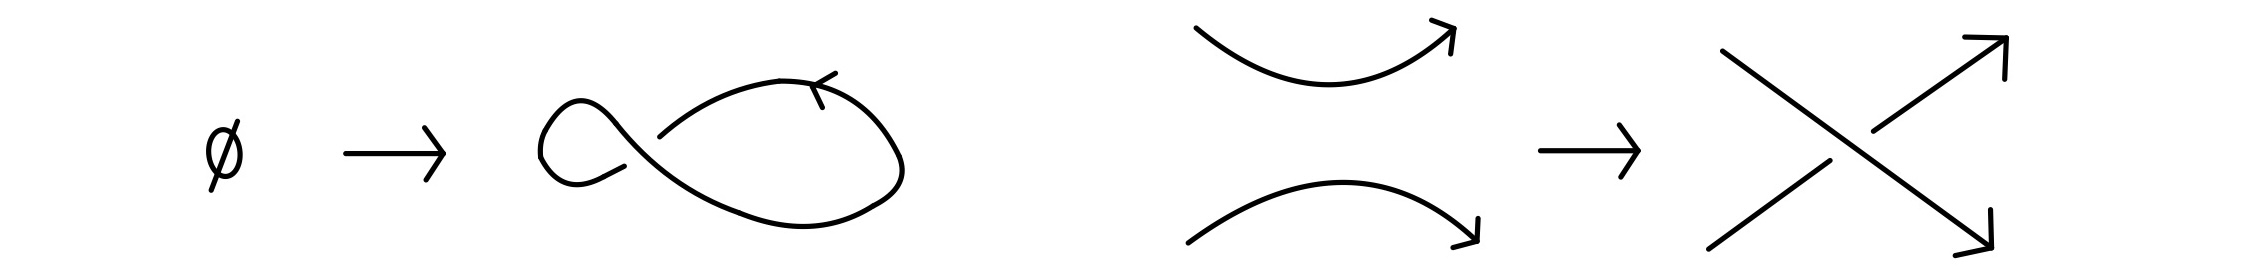
\includegraphics[scale=0.2]{figures/moves.jpeg}
    \caption{Elementary birth (a) and saddle (b) moves between transverse link diagrams}
    \label{fig:moves}
\end{figure}
Figure \ref{fig:tra}(b) is a transverse representative of $K_m$ because it is the transverse pushoff of a Legendrian realization \ref{fig:tra}(a) 
\cite{geiges2008contact}.
\begin{figure}[H]
    \centering
    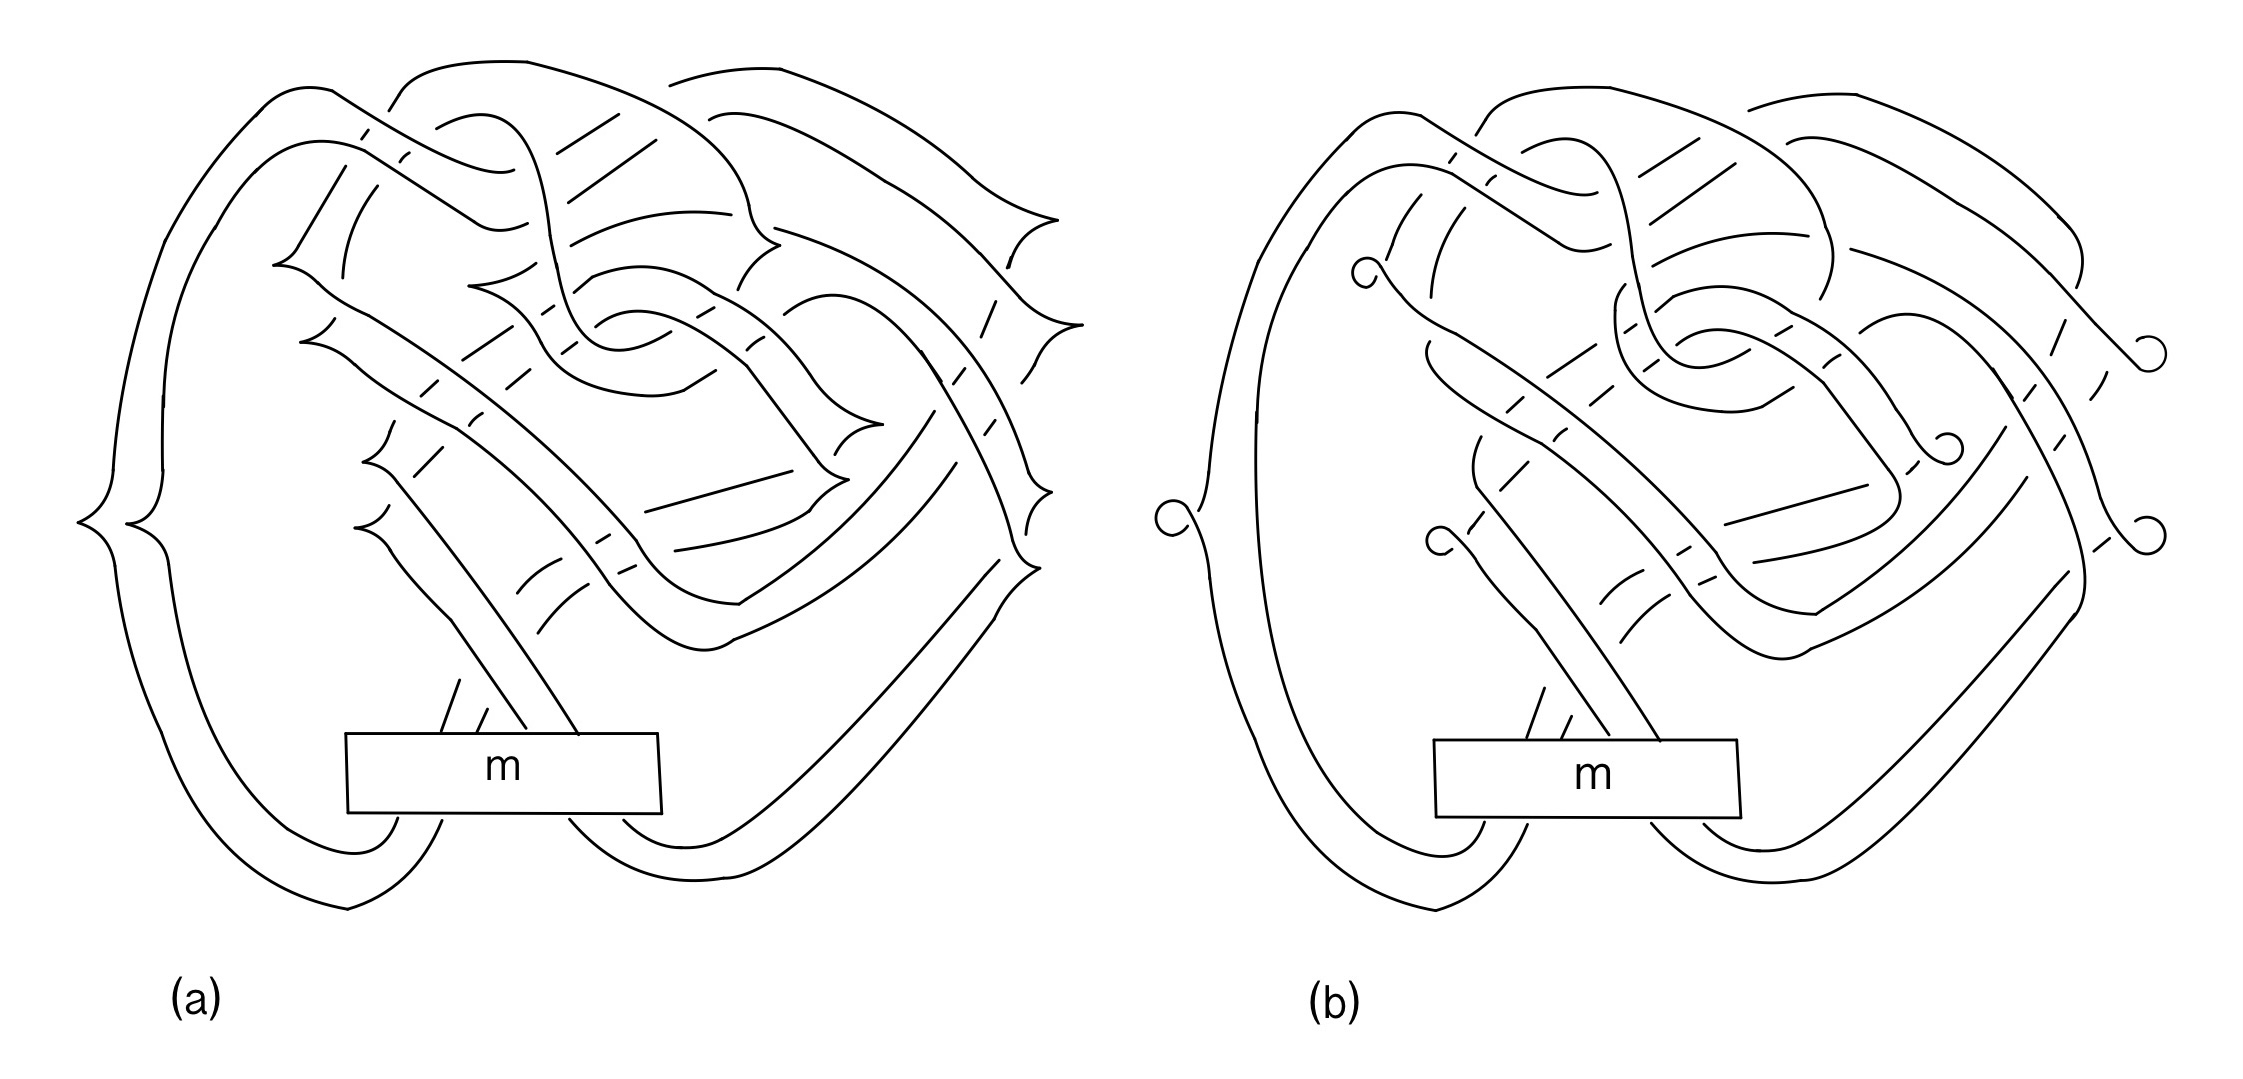
\includegraphics[scale=0.18]{figures/tra.jpeg}
    \caption{Legendrian (a) and transverse (b) representatives of $K_m$}
    \label{fig:tra}
\end{figure}
\begin{figure}[H]
    \centering
    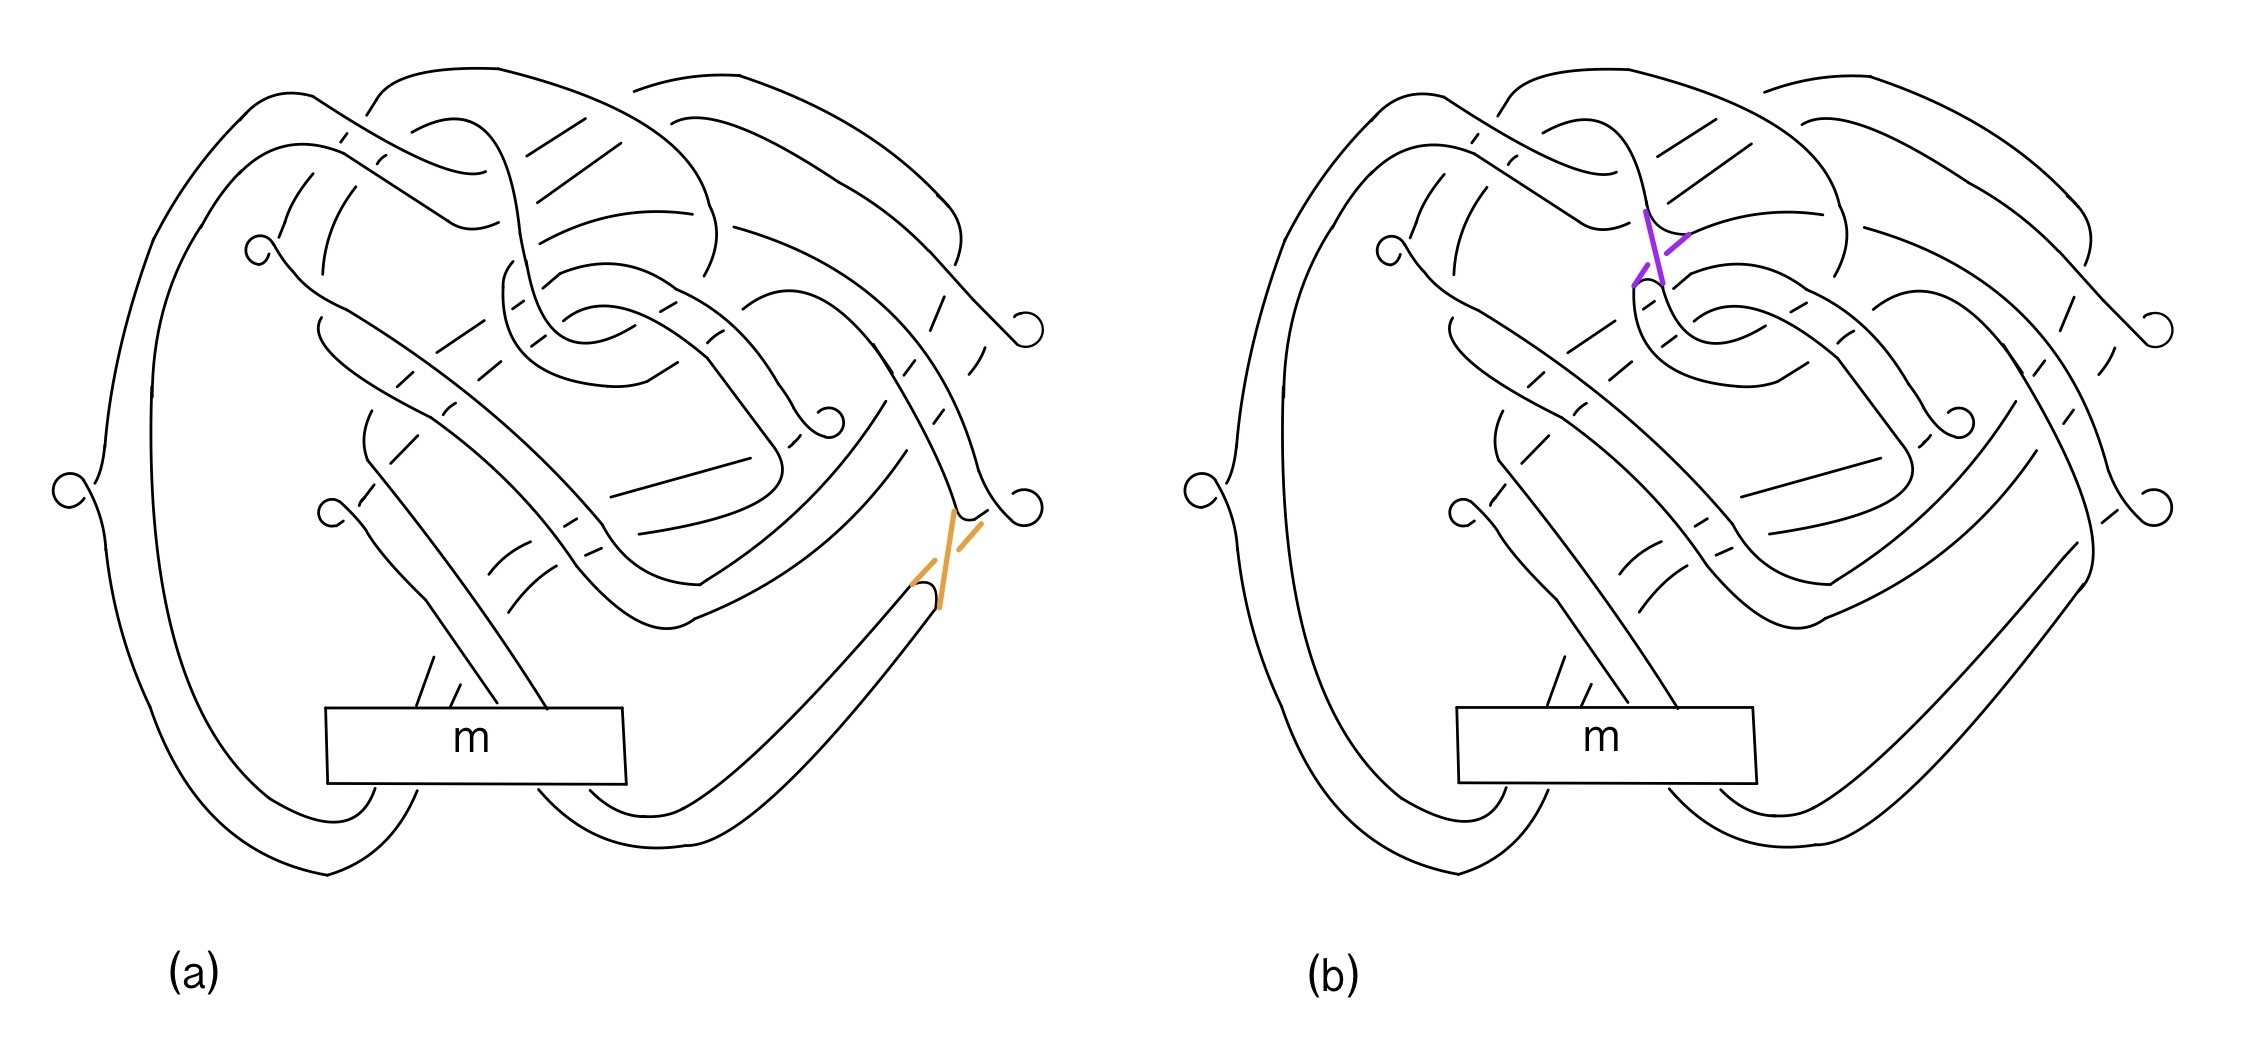
\includegraphics[scale=0.18]{figures/band.jpeg}
    \caption{Saddle moves on transverse link diagrams}
    \label{fig:band}
\end{figure}
Moreover, the band moves depicted in Figure \ref{fig:band} corresponds to the previous band surgeries. These moves are also cobordisms between $K_m$ and a pair of positively transverse unknots. Thus, using Lemma \ref{cob}, we construct symplectic disks which are smoothly isotopic to $D$ and $D'$.
\\ \\
\textbf{Proof of B} \\
To establish the topological isotopy, we use a result of Conway and Powell.
\begin{defn}A ribbon disk $D$ is $\Z$-homotopy ribbon, if $$
\pi_1(\B^4 \setminus \nu(D)) \cong \Z
$$
An oriented knot is $\Z$-homotopy ribbon, if it bounds a $\Z$-homotopy ribbon disk.
\end{defn}
\begin{thm}\cite{conway-powell}\label{conwa} Any two $\Z$-homotopy ribbon disks of a $\Z$-homotopy ribbon knot, are ambiently topologically isotopic relatively to the boundary.
\end{thm}
We will construct Kirby diagrams for $\estd$ and $\estdi$. The smooth structure of $D$ and $D'$ is defined via the handle decomposition with two minima and one saddle. As explained in sections \ref{driii} \ref{acqua}, we draw a dotted circle on the boundary of each $0$-handle. Then each band corresponds to a $2$-handle of the exterior. The resulting diagrams are depicted in Figures \ref{fig:comp1}(a) and \ref{fig:comp21}(a).
In order to compute the fundamental groups, it is really helpful to isotope the pair of $1$-handles to a two component unlink. The pictures below, illustrate the desired sequence of isotopies and Kirby moves. Observe that step (c) of \ref{fig:comp1} and step (b) of \ref{fig:comp21} involve $1$-handle slides.
Other steps are isotopies.
\begin{figure}[H]
    \centering
    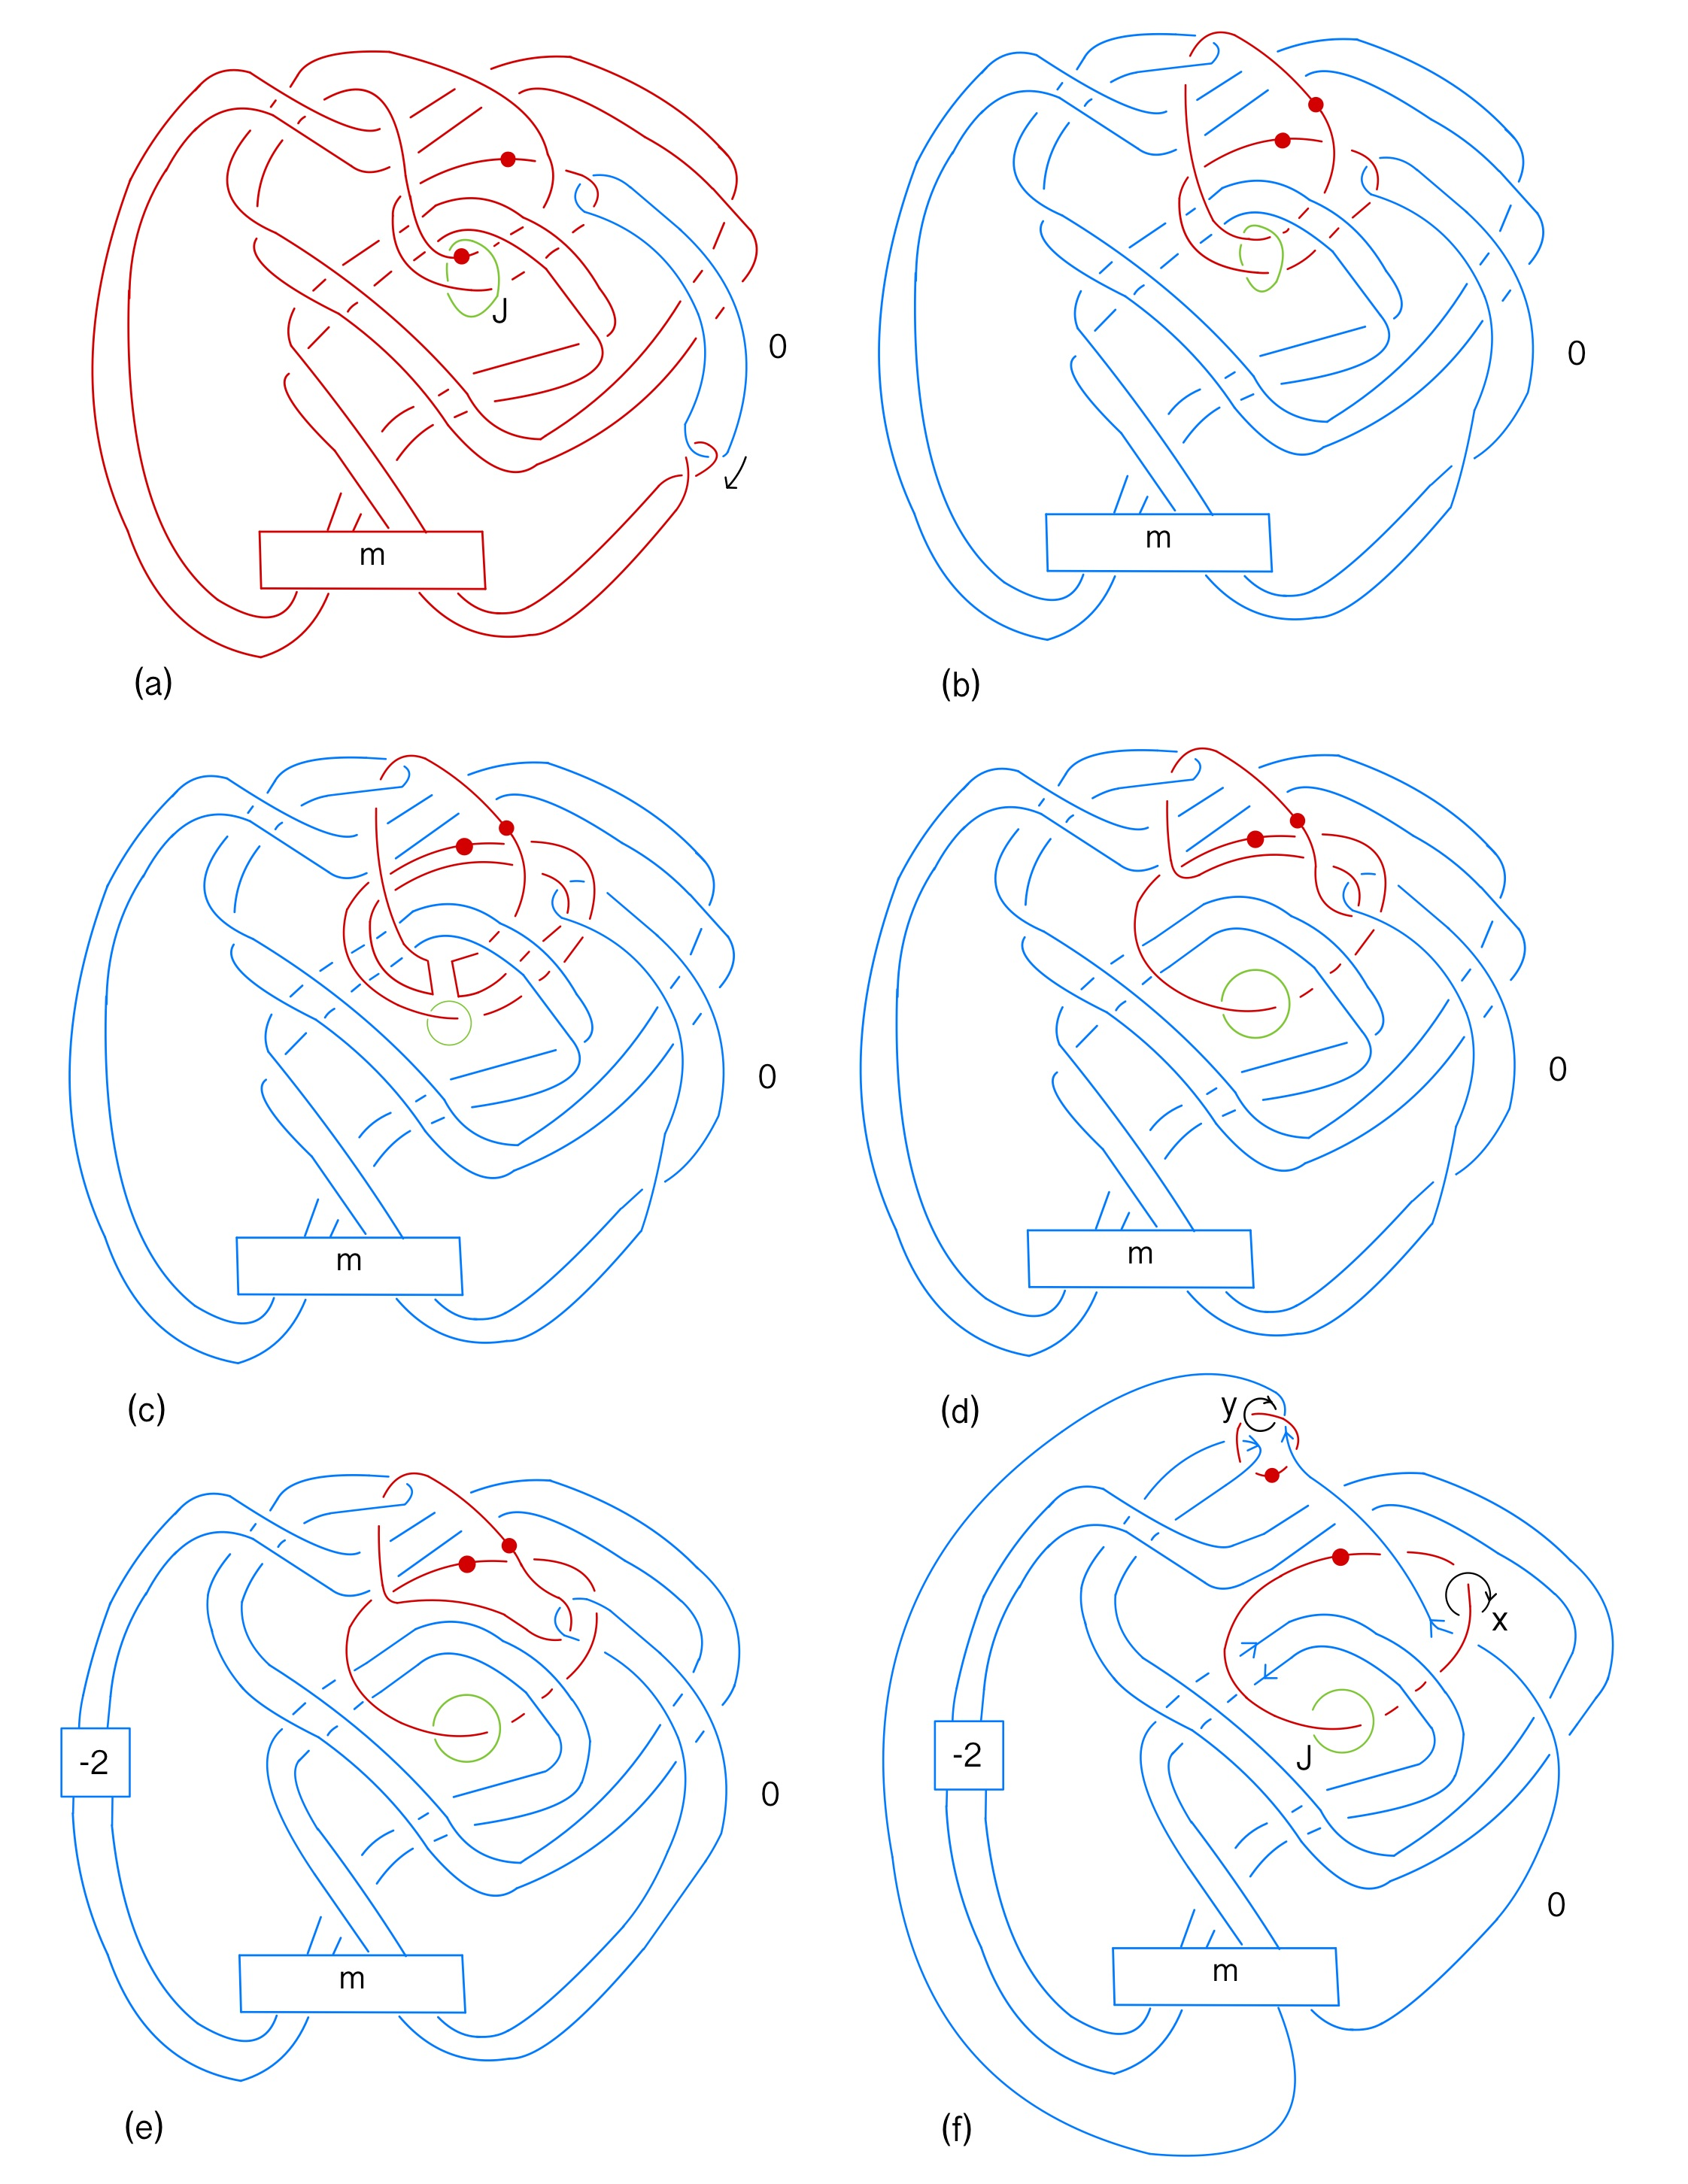
\includegraphics[scale=0.2]{figures/comp1.jpeg}
    \caption{Kirby diagram of $\estd$}
    \label{fig:comp1}
\end{figure}
\begin{figure}[H]
    \centering
    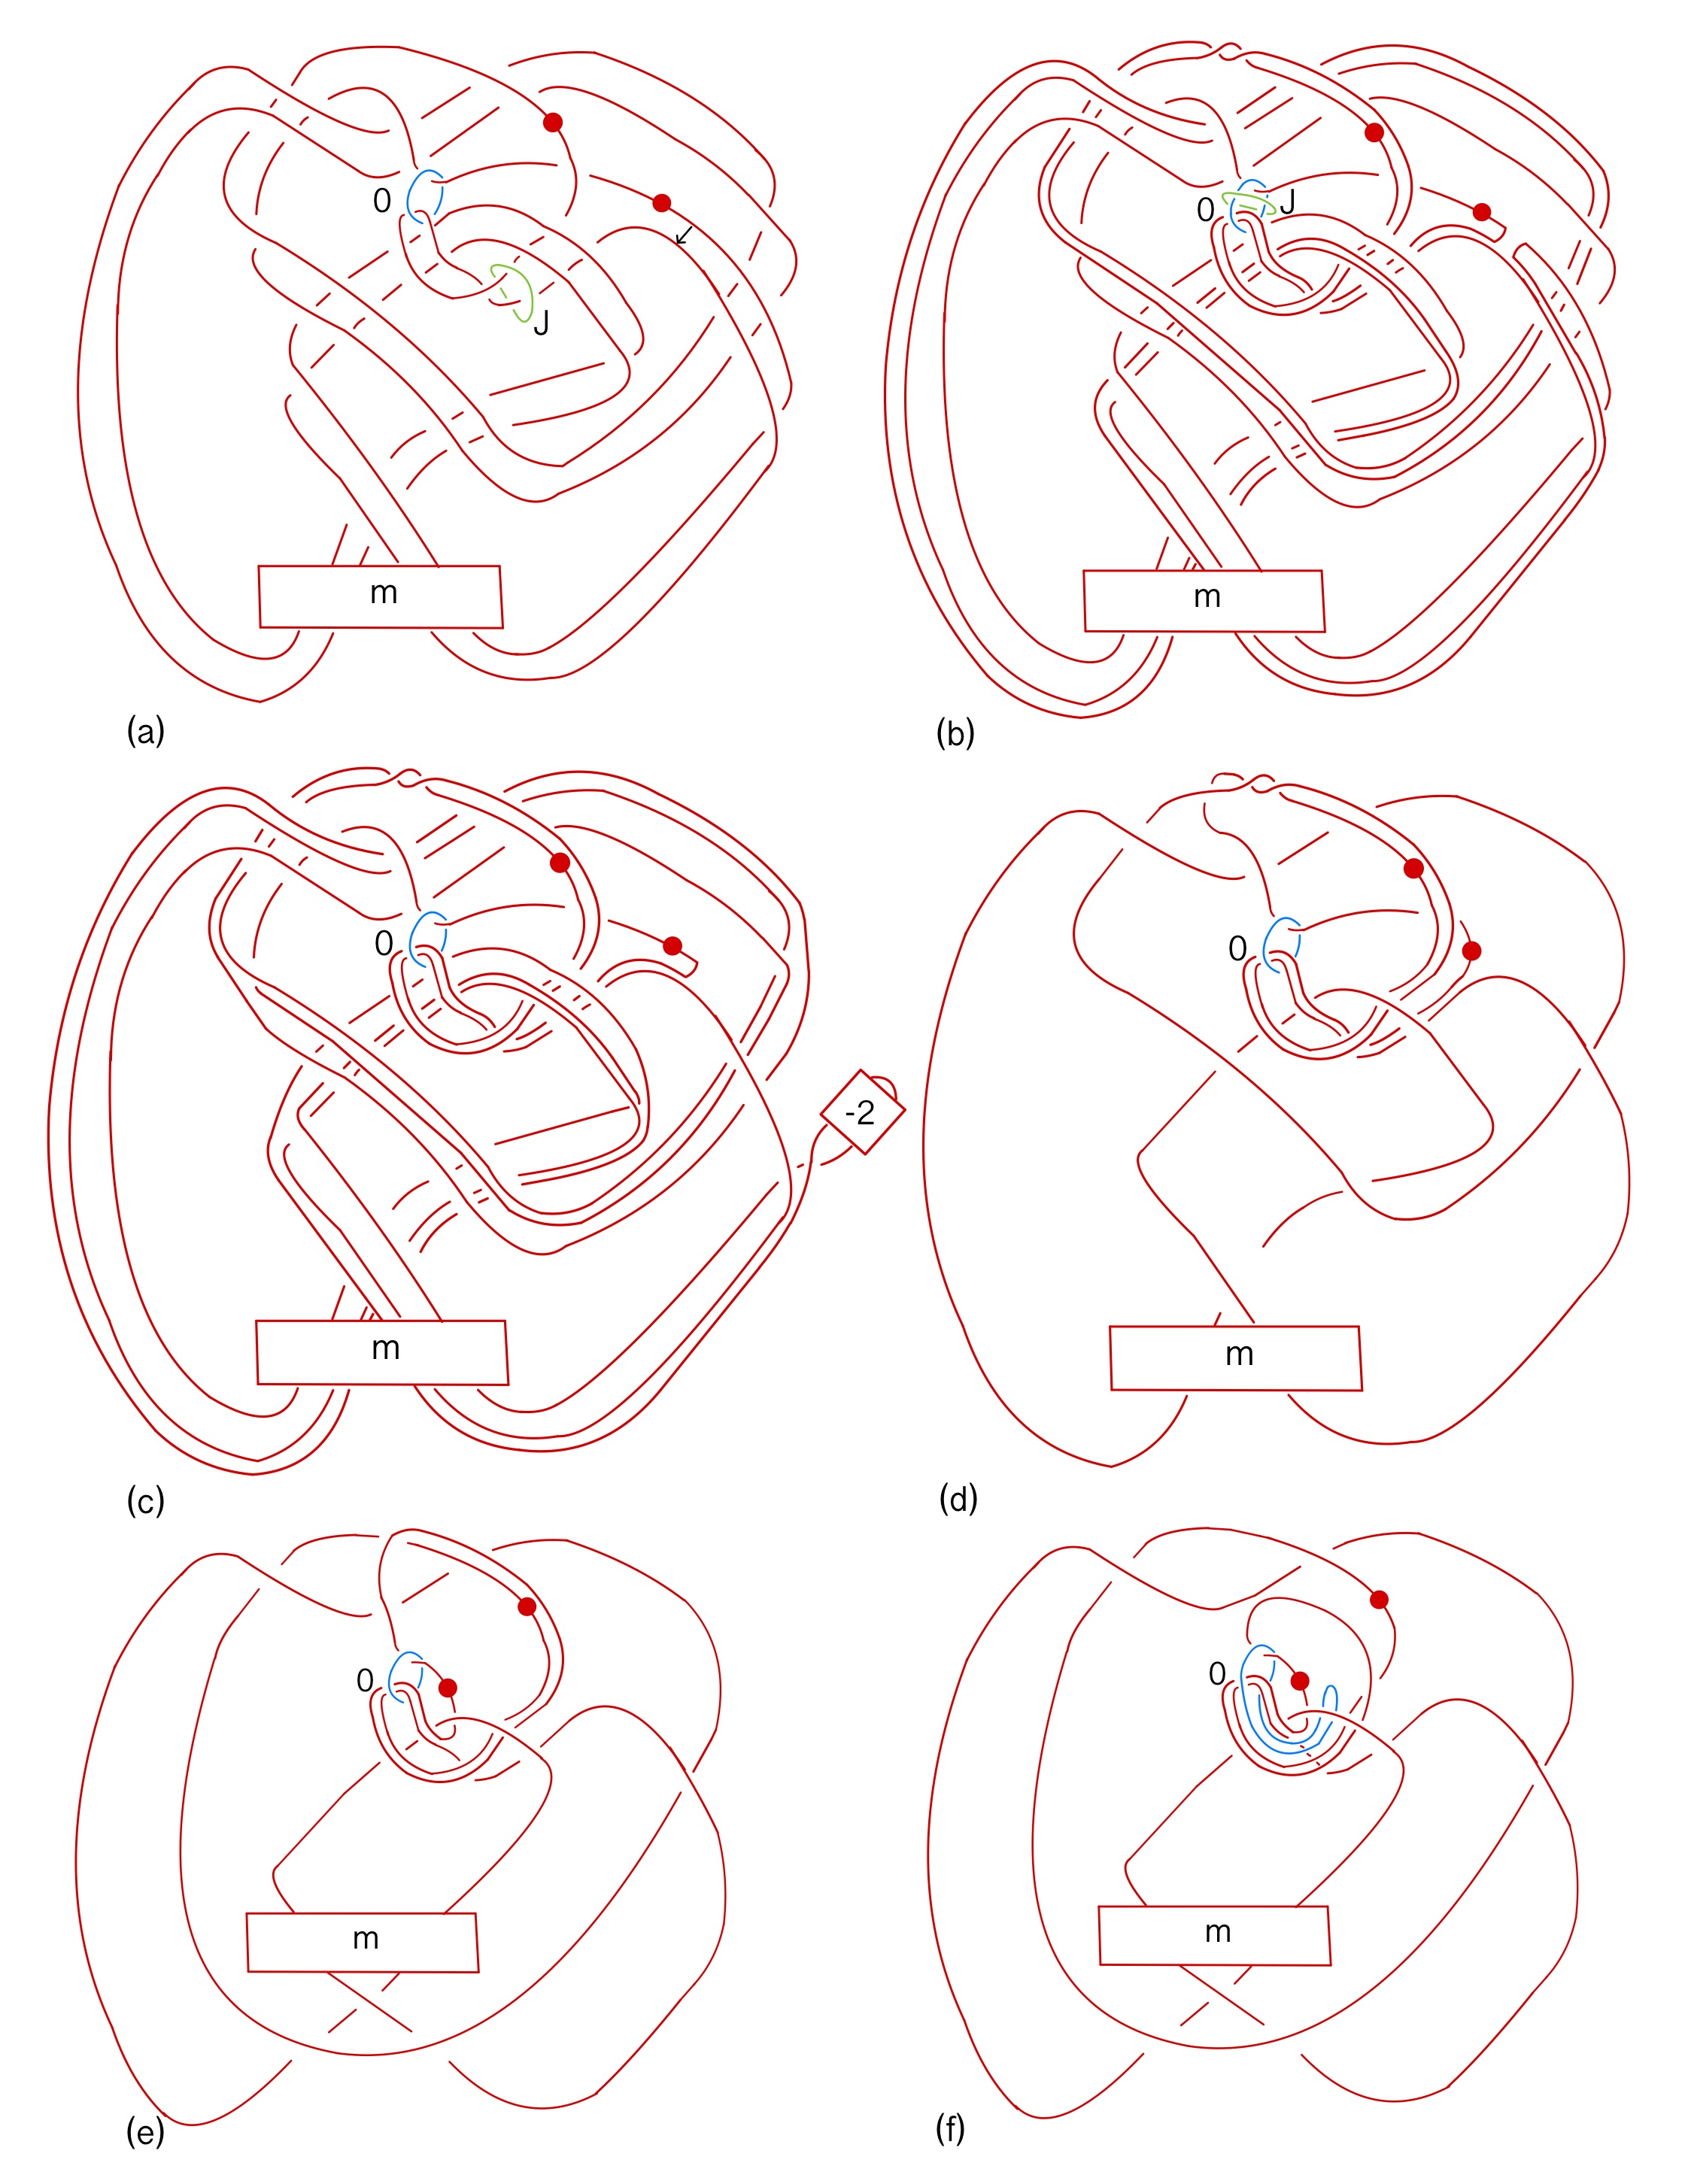
\includegraphics[scale=0.2]{figures/comp21.jpeg}
    \caption{Kirby diagram of $\estdi$}
    \label{fig:comp21}
\end{figure}
\begin{figure}[H]
    \centering
    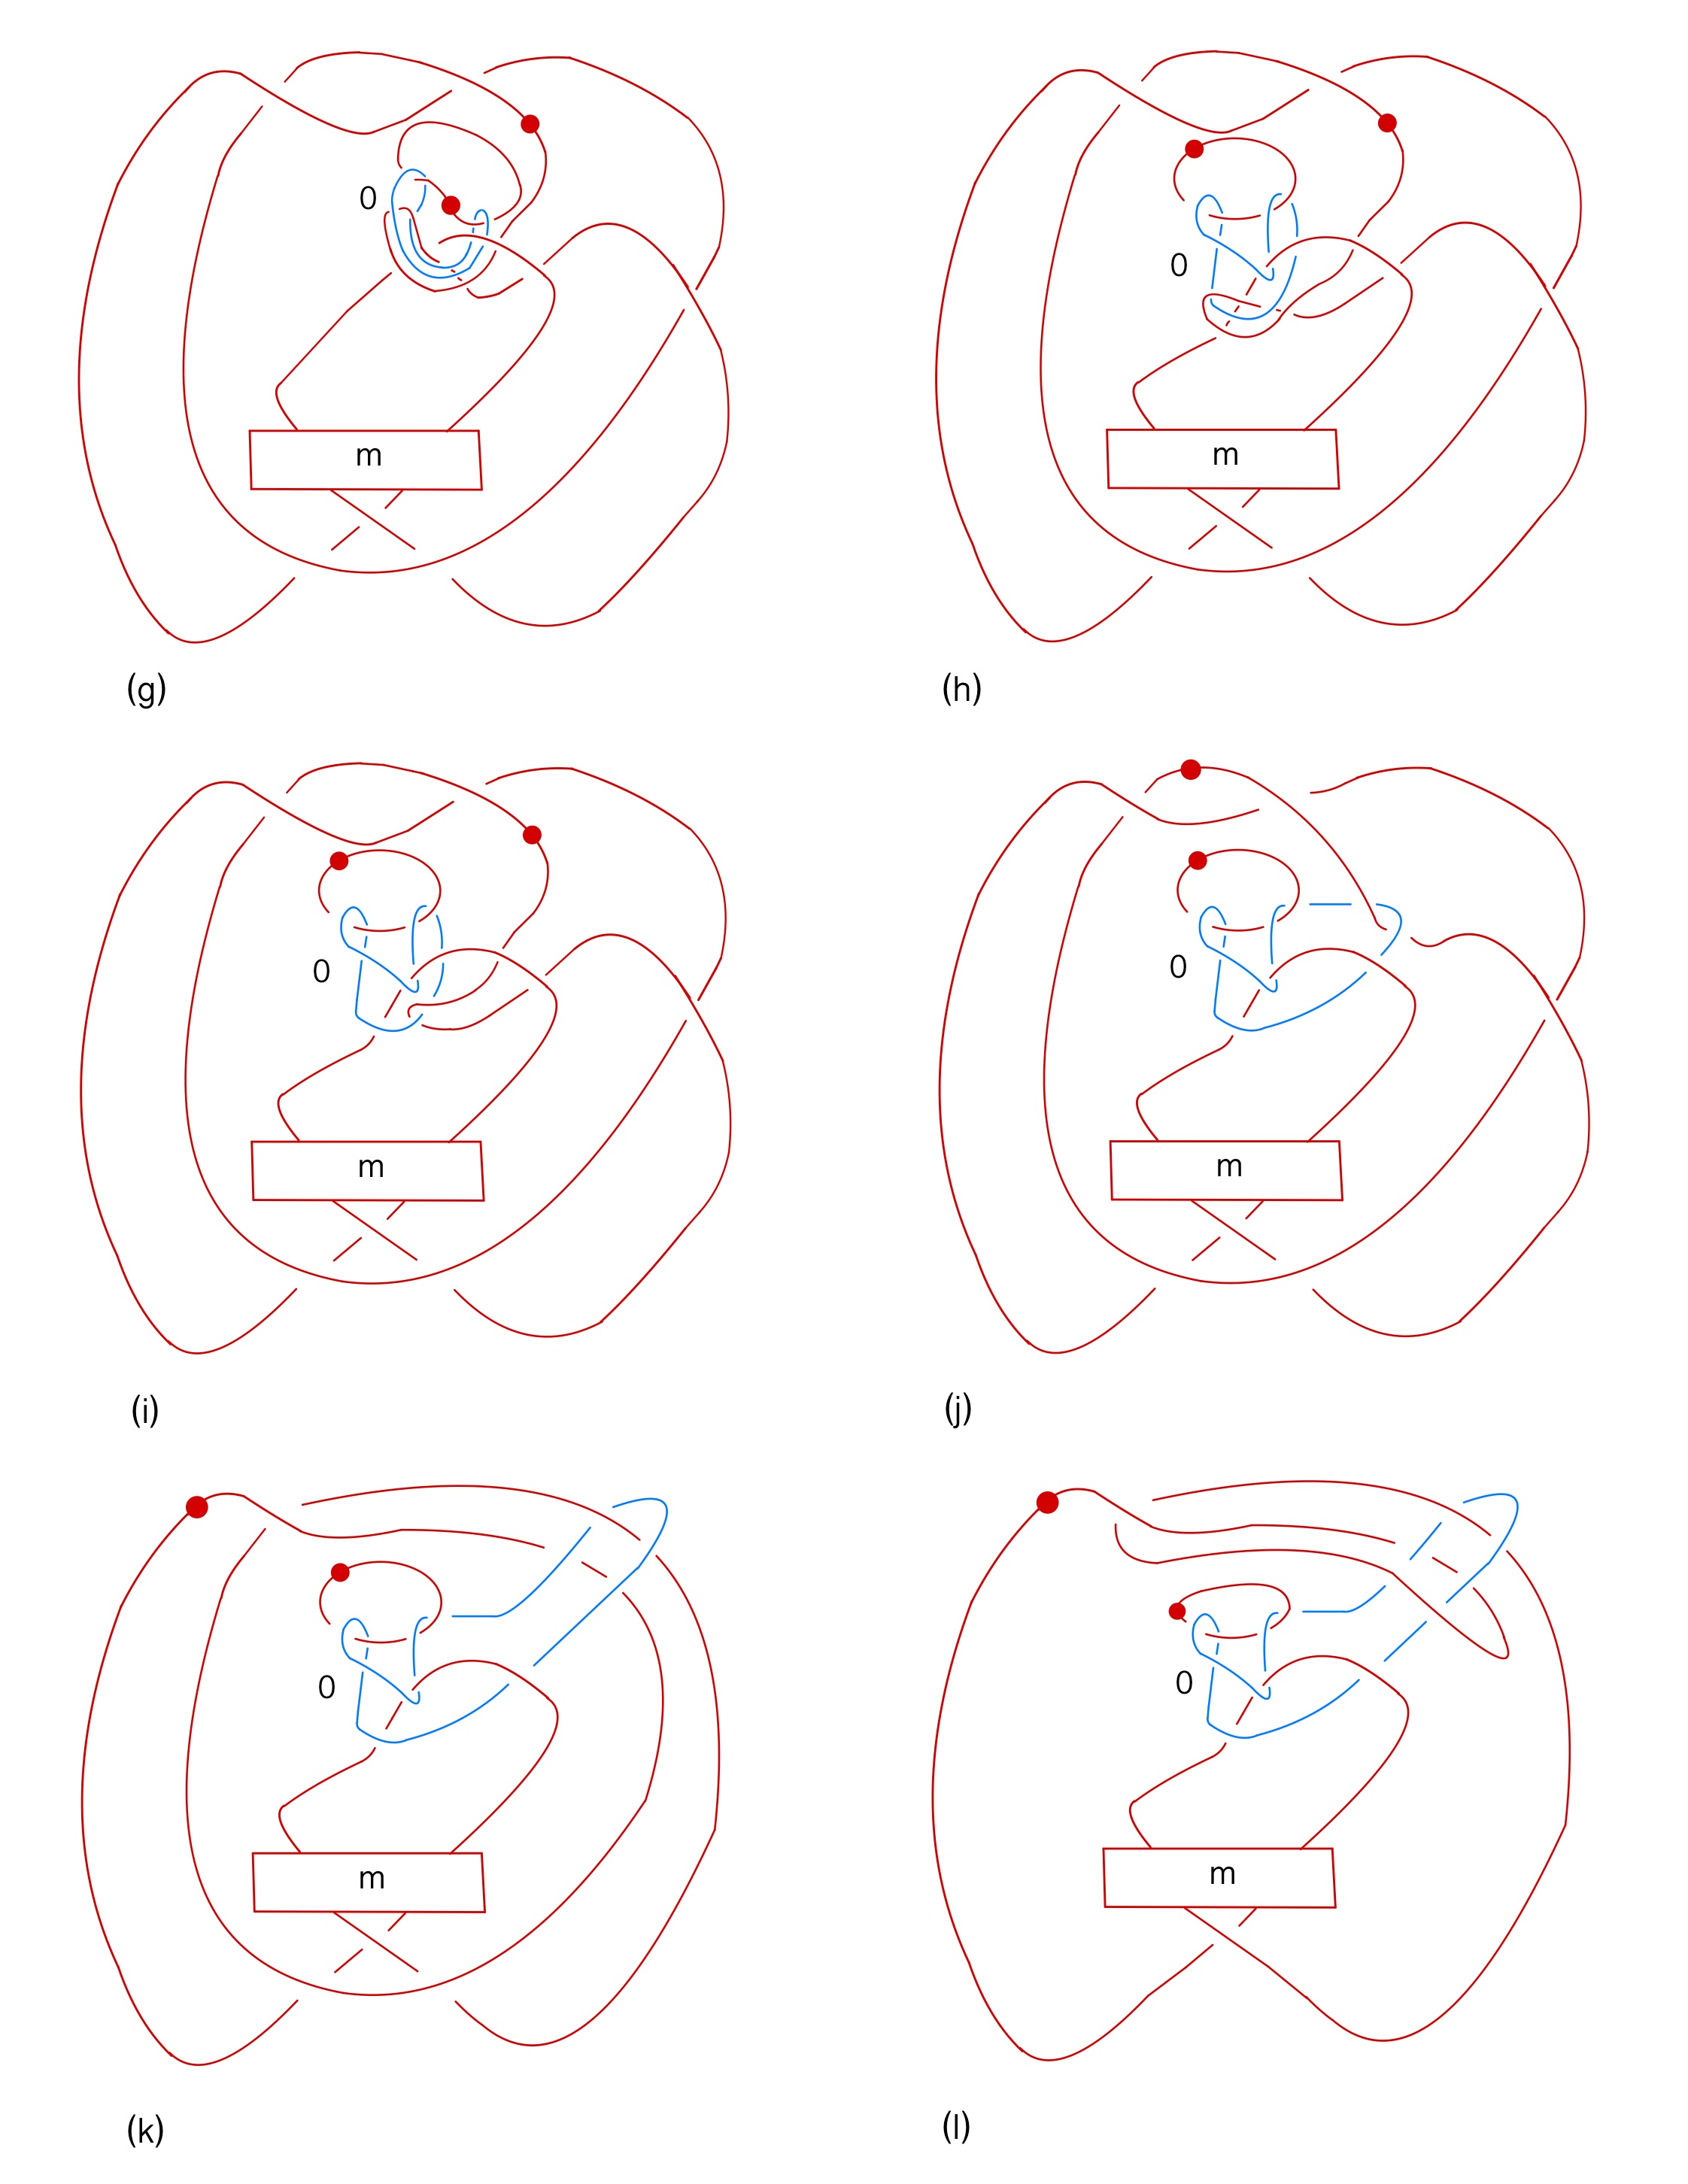
\includegraphics[scale=0.2]{figures/comp22.jpeg}
    \caption{Simplifying the Kirby diagram of $\estdi$}
    \label{fig:comp22}
\end{figure}
\begin{figure}[H]
    \centering
    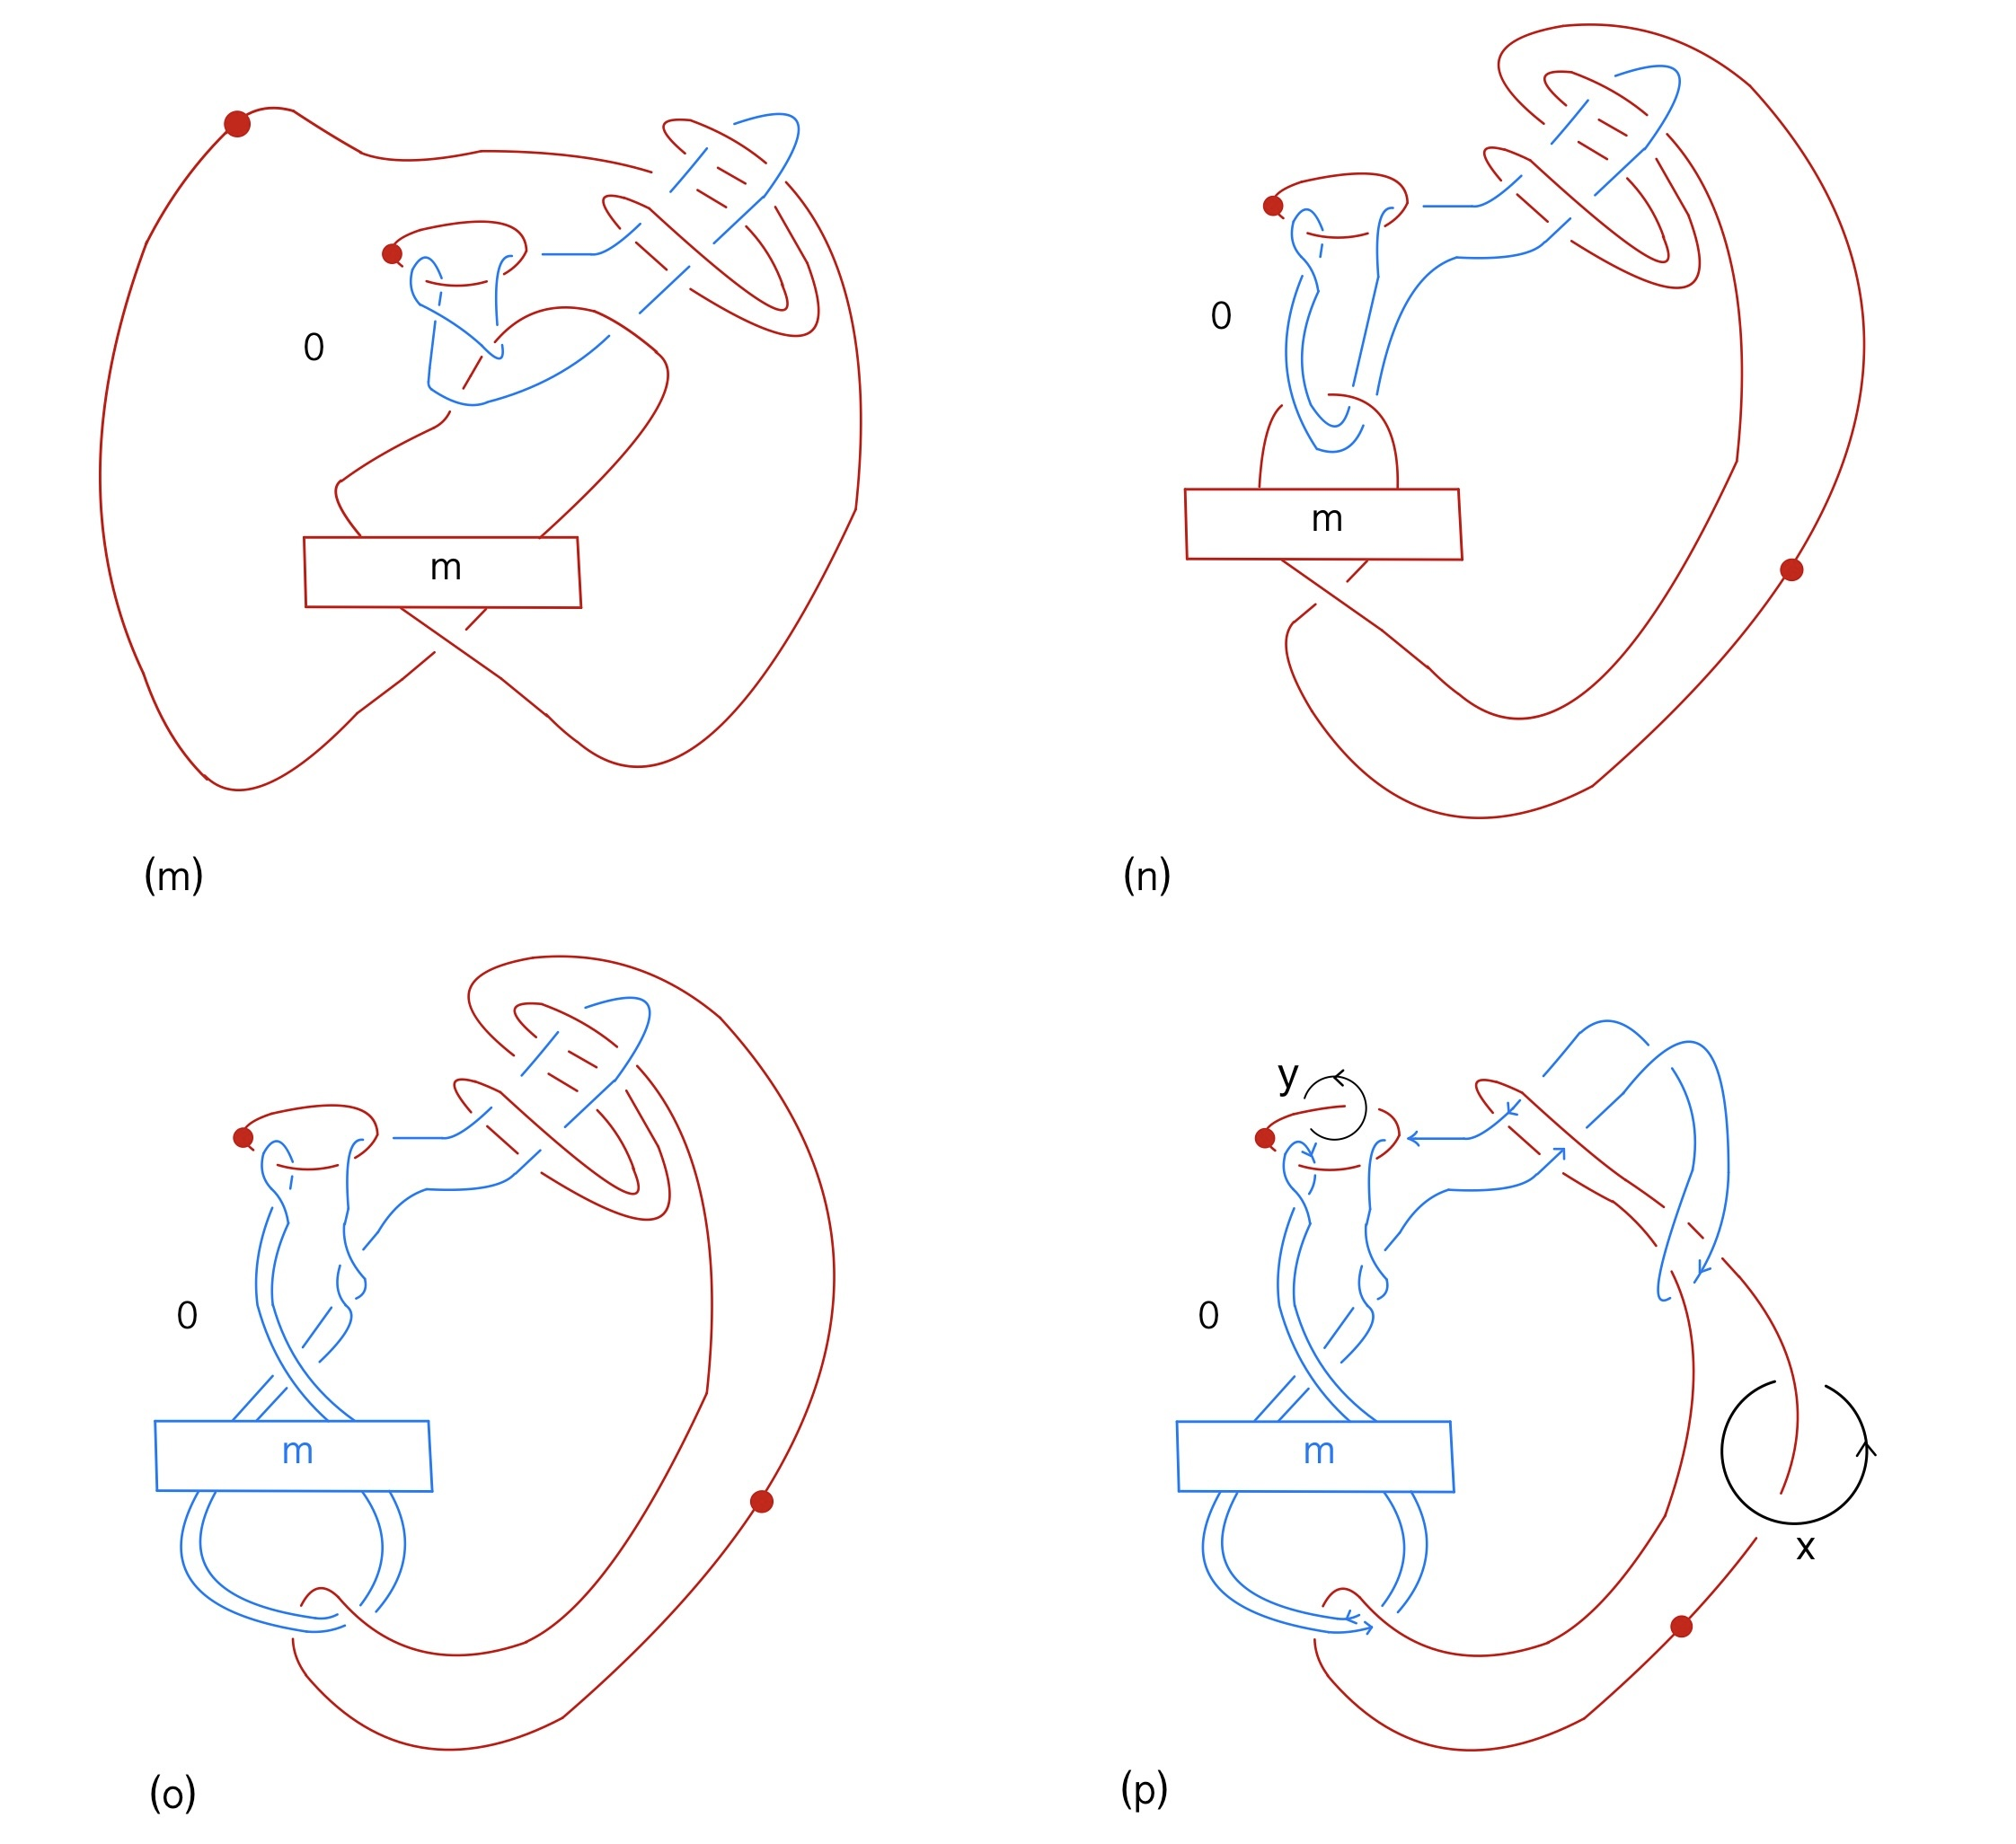
\includegraphics[scale=0.2]{figures/comp23.jpeg}
    \caption{Further simplification of the Kirby diagram of $\estdi$}
    \label{fig:comp23}
\end{figure}
The fundamental group is computed using the method outlined in section \ref{rec}.
Figures \ref{fig:comp1}(f) and \ref{fig:comp23}(p) are decorated with oriented generators and oriented attaching curve of the $2$-handle. We have:
$$
\pi_1(\estd) = \langle x, y  \quad | \quad xy^{-1}xyx^{-1}\rangle \cong \Z
$$
$$
\pi_1(\estdi) = \langle x, y \quad | \quad x^{-1}x^{-1}xyy^{-1}\rangle \cong \Z
$$
Therefore, Conwell and Powell's theorem \ref{conwa} estabilishes the topological isotopy.
\newpage
\textbf{Proof of (C)} \\
Assume, for the sake of contradiction, that there exists a diffeomorphism 
$\varphi:  \B^4 \rightarrow \B^4$
such that
$$\varphi(D') = D
$$
We establish the following technical Lemma.
\begin{lem}\label{technic} Suppose $m = 0$ or $m < < 0$\footnote{Here we mean all but finitely many $m<0$}. Let $\varphi: \s^3 \rightarrow \s^3$ be a diffeomorphism carrying $K_m$ to itself. Then $\varphi$ restricts to the identity on $\s^3 \setminus \inter$, up to isotopy.
\end{lem}
\proof Let $\varphi : \s^3 \rightarrow \s^3$ as defined above.
Define $U = \s^3 \setminus \inter$ and $V = \nu(K_m)$
Observe that, up to isotopy, we may assume the following $$
\varphi(U) = U \qquad \varphi(V) = V
$$
We construct an isotopy by gluing two isotopies defined on the closed sets $U, V$.
Note that $\s^3 \setminus K_m $ can be expressed as $ (\s^3 \setminus K_0)_{-\frac{1}{m}}(\gamma)$, where $\gamma$ is the purple curve shown in Figure \ref{fig:hyper}.
\begin{figure}[H]
    \centering
    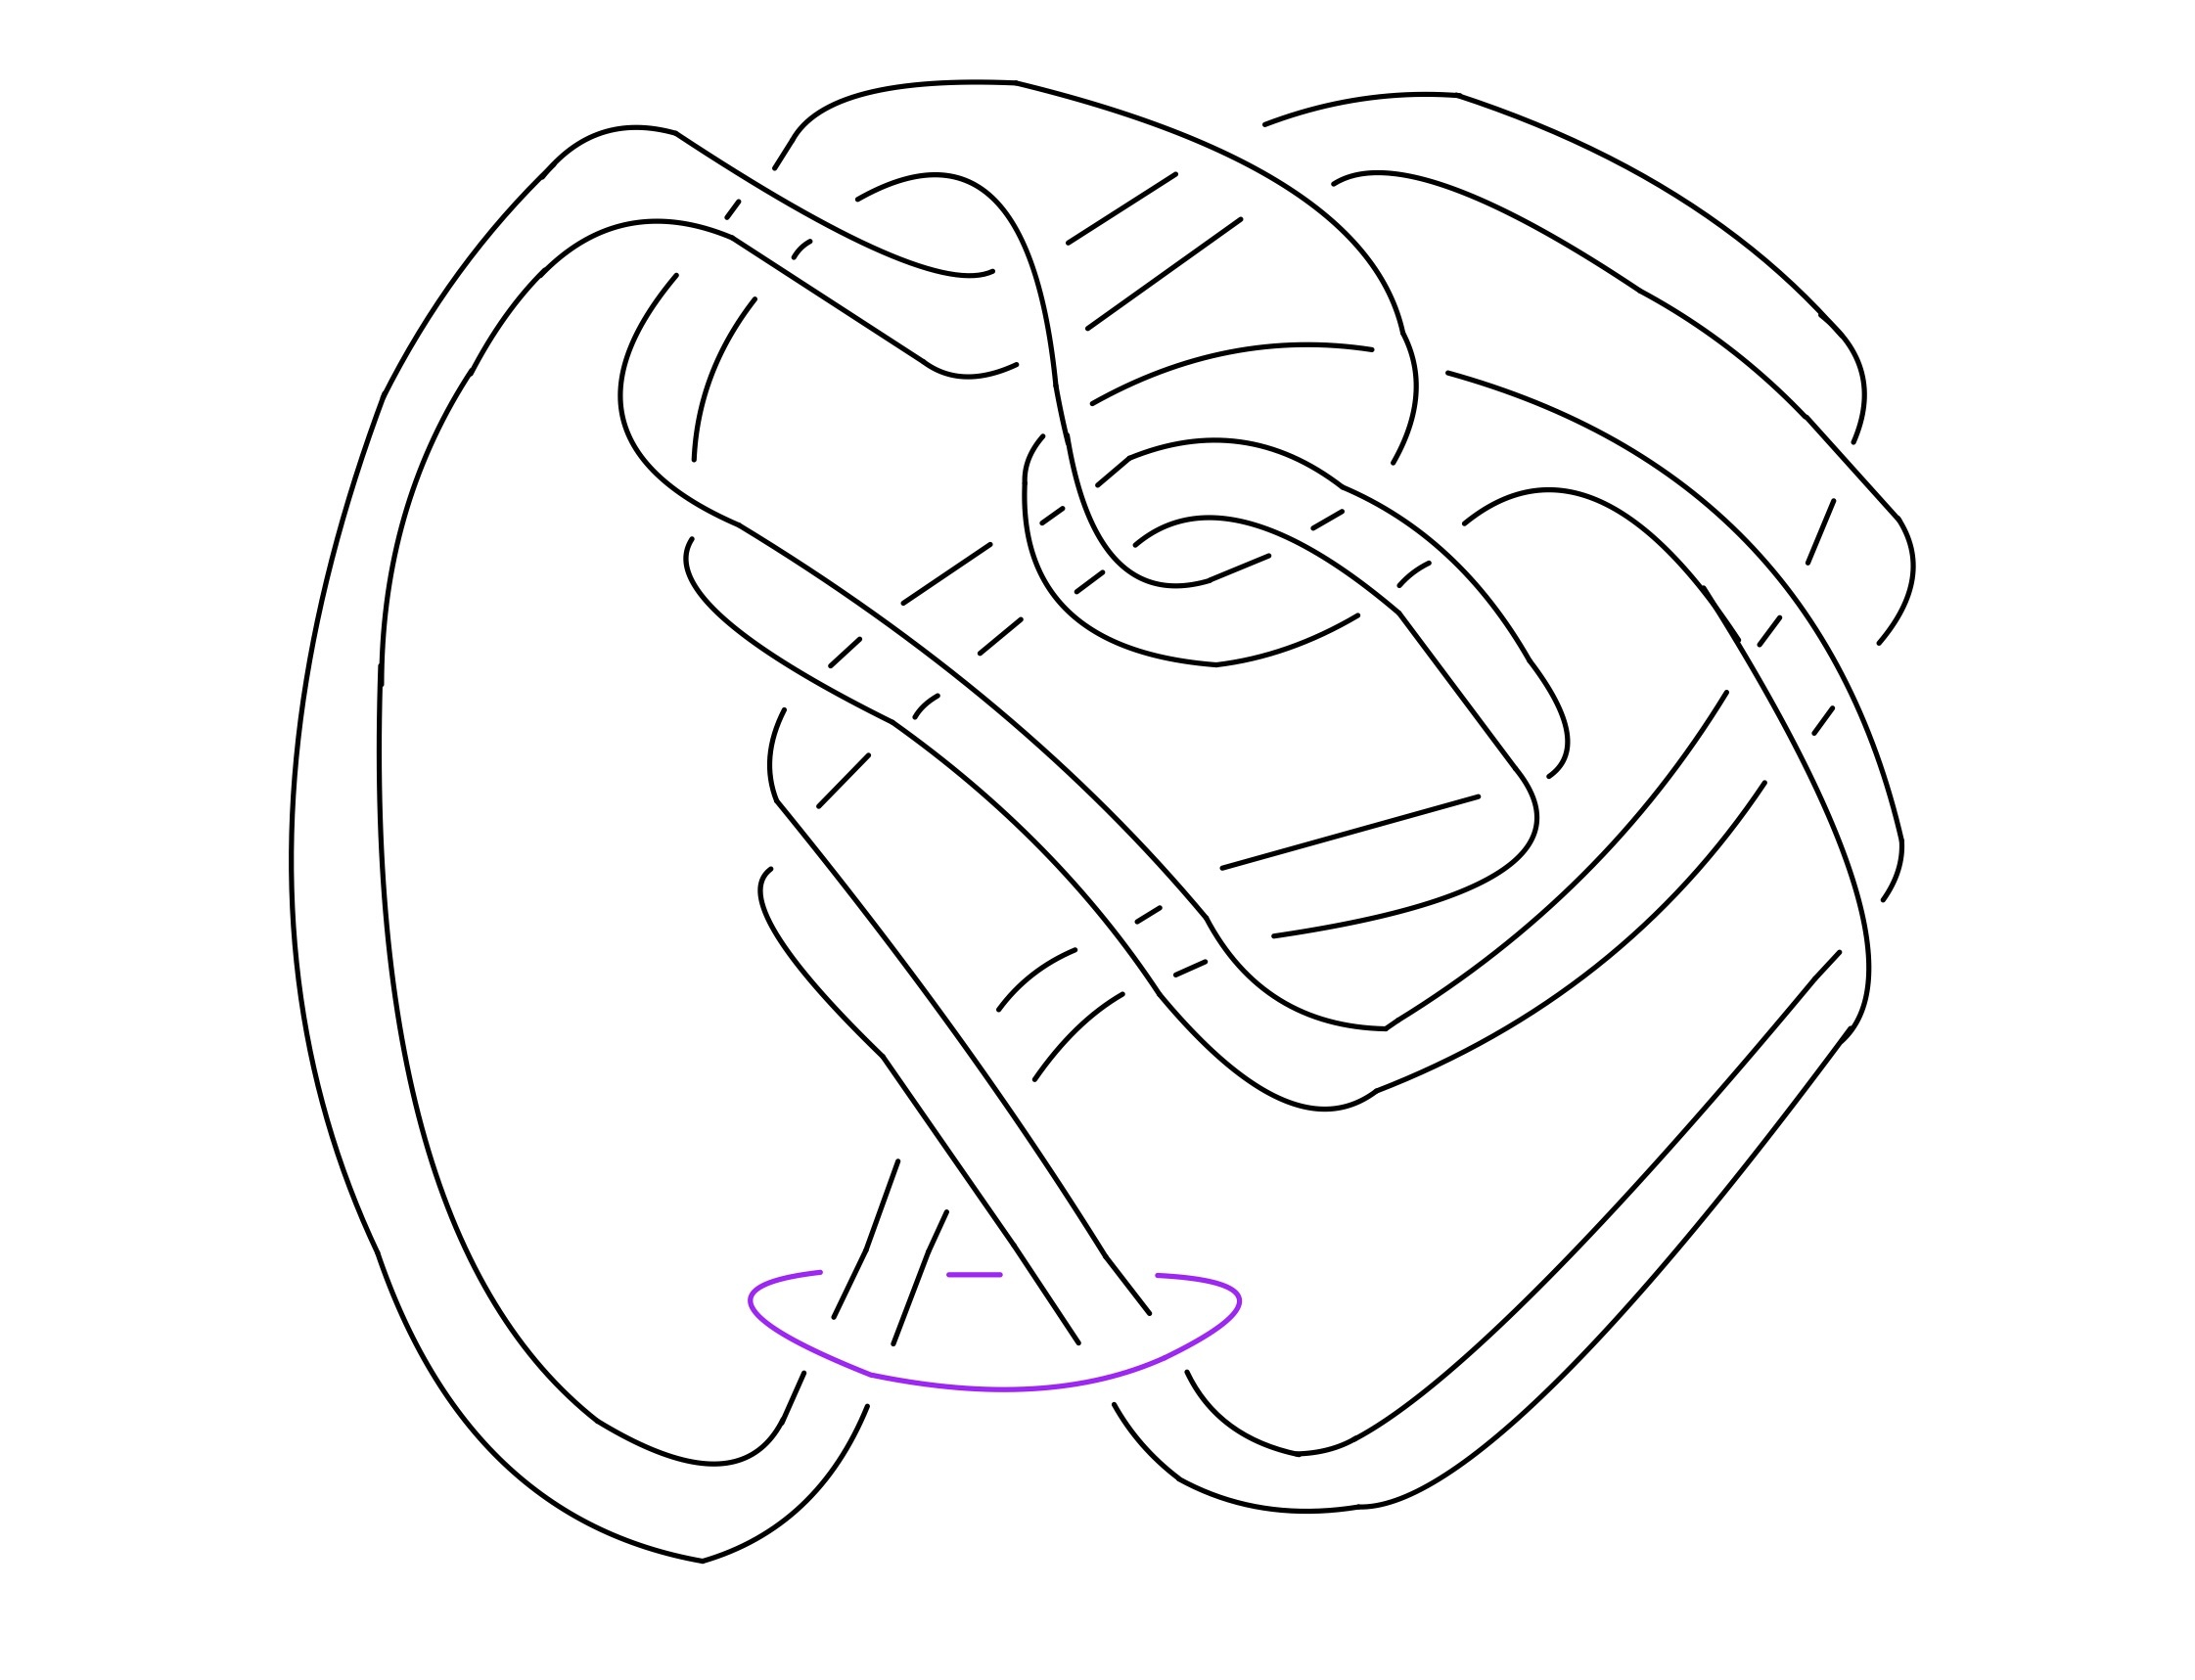
\includegraphics[scale=0.12]{figures/hyper.jpeg}
    \caption{$K_0$ and a curve $\gamma$ in its exterior, used to analyze the hyperbolic structure}
    \label{fig:hyper}
\end{figure}
\begin{defn}
A hyperbolic manifold $M$ is defined to be asymmetric if $$Isom(M) = 1$$.
\end{defn} 
\begin{cla}
$\s^3 \setminus K_0$ and $\s^3 \setminus (K_0 \cup \gamma)$ are asymmetric hyperbolic $3$ manifolds.
\end{cla}
This claim is verified using Snappy, with the computations detailed in the appendix \ref{app}.
It is well known that all hyperbolic manifolds, arising from knot complements, are $1$-cusped \cite{thurston1997geometry}. The following Lemma guarantees that $\s^3 \setminus K_m$ is also a hyperbolic asymmetric $3$ manifold for all but finitely many values of $m < 0$.
\begin{lem} \cite{dhl}\label{cuspi}
Let $M$ be an asymmetric, $1$ - cusped, hyperbolic $3$ manifold. \\
Then all but finitely many Dehn fillings of $M$ are hyperbolic and asymmetric.
\end{lem}
Let $m \leq 0$ be a value satisfying the conditions of the previous Lemma.
As the inclusion of $Isom(M)$ into $Diff(M)$ is a homotopy equivalence for hyperbolic $3$ manifolds $M$ \cite{gabai:smale},  $$
\restr{\varphi}{\s^3 \setminus K_m} \in Diff(\s^3 \setminus K_m)
$$is isotopic\footnote{In this setting, homotopic diffeomorphisms are isotopic by Waldhausen's work \cite{Waldhausen1968}.} to the identity. Restricting this isotopy gives $\restr{\varphi}{U}$ is isotopic to $id_U$.
Finally, we glue the latter with an isotopy of $\restr{\varphi}{V}$ which leaves $\s^3 \setminus \nu(K_m)$ untouched. Hence the thesis.
\endproof
Consider $\restr{\varphi}{\s^3}$. By the previous Lemma , we can assume, up to isotopy, that $$
\restr{\varphi}{\s^3 \setminus \inter} = id_{\s^3 \setminus \inter}
$$
Then we can extend the isotopy to the whole $\B^4$, requiring that it is supported away from $D$. \\
Our strategy involves finding a knot $J \subseteq \s^3 \setminus K$ that bounds a disk in $\B^4 \setminus D'$ but not in $\B^4 \setminus D$.
Consider the green curve $J$ drawn in figure \ref{fig:km}. \\
\begin{cla}$J$ bounds an embedded disk $\mathfrak{D}'$, which is disjoint from $D'$.
\end{cla}
We analyze $J$ within the Kirby diagram of $\B^4 \setminus \interd$ as in figure \ref{fig:comp21} (a) and (b). Since $J$ does not pass through the $1$-handles, it bounds a disk embedded in $\estdi$, which is tautologically disjoint from $D'$.
\\ \\ 
As $\varphi$ fixes $\s^3 \setminus \inter$, in particular, $J$ is fixed. \\
Thus $$
\varphi(\mathfrak{D}') = \mathfrak{D} 
$$is a disk with $$
\partial \mathfrak{D} = J
$$
Moreover, it is disjoint from $D$, otherwise $\varphi^{-1}(\mathfrak{D}\cap D) = \mathfrak{D'} \cap D' \neq \emptyset$, that is not possible due to construction. 
\section{Double Branched Cover Argument} \label{buffet}
We employ the double branched cover construction to obstruct the existence of $\mathfrak{D}$. \\ \\ We build $\Sigma(\B^4, D)$ following the instructions from section \ref{covers}. 
In order to draw a Kirby diagram for $\Sigma(\B^4, D)$, we use the following strategy which is divided into three steps. \\ \\
\textbf{Step 1}: Draw a Kirby for the disk exterior (It is depicted in Figure \ref{fig:comp1}(a)-(f)).\\ \\
\textbf{Step 2}: By examining the $\Z/2\Z$ action on $1$-handles, draw a Kirby diagram for the double covering of $\estd$. \\ \\
\textbf{Step 3}: Fill the branch locus by adding a $2$-handle, that will cancel itself together with a $1$-handle. \\ \\
 First, we describe a Kirby diagram for the double covering of $\estd$. Let $\varphi: \pi_1(\estd) \rightarrow \Z/2\Z$ be the surjective map which defines such covering. 
Consider Figure \ref{fig:comp1}(f). Recall that $\pi_1(\estd)$ is generated by $y$, that is the core curve of the upper $1$-handle $H_1$. Thus $\varphi(y) = 1$. Since we performed a handle slide in step (c) of Figure \ref{fig:comp1}, the core curve of the other $1$-handle, lies in $2\Z = Ker(\varphi)$. \\ Observe that $\B^4 \cup H_1 \cong \s^1 \times \B^3$ is double covered by $\s^1 \times \B^3$ via the map $(e^{it}, x) \rightarrow (e^{2it}, x)$. Therefore, $H_1$ lifts to a single $1$-handle. On the other hand, each of the remaining handles lift to two copies of them. 
\begin{note} A bare hand computation (via the double strand notation), shows that the $2$-handle framings are preserved on each lifted copy.
\end{note}
So we need to juxtapose two copies of Figure \ref{fig:branch1}(a), as suggested on the right side. Figure \ref{fig:branch1}(b) depicts the Kirby diagram of the double covering of $\B^4 \setminus D$. Finally, we fill the branch locus $D$, by removing a $1$-handle as in Figure (c). That is the Kirby diagram of $\Sigma(\B^4, D)$. Notice that the simmetry makes the $\Z/2\Z$ action evident. \\ \\
Next, we simplify the diagram. In step (d), we slide a $2$-handle over the other. In Figure \ref{fig:branch3}(f) we add a curl. Then in step (g) we perform a $2$-handle slide again (we report only a local picture). In Figure \ref{fig:branch4}(h) we cancel the handle pair. The other steps (i)-(n) are just isotopies. Throughout this process, we track the green curve $\tilde{J}$, an arbitrary lift of $J$.
\begin{figure}[H]
    \centering
    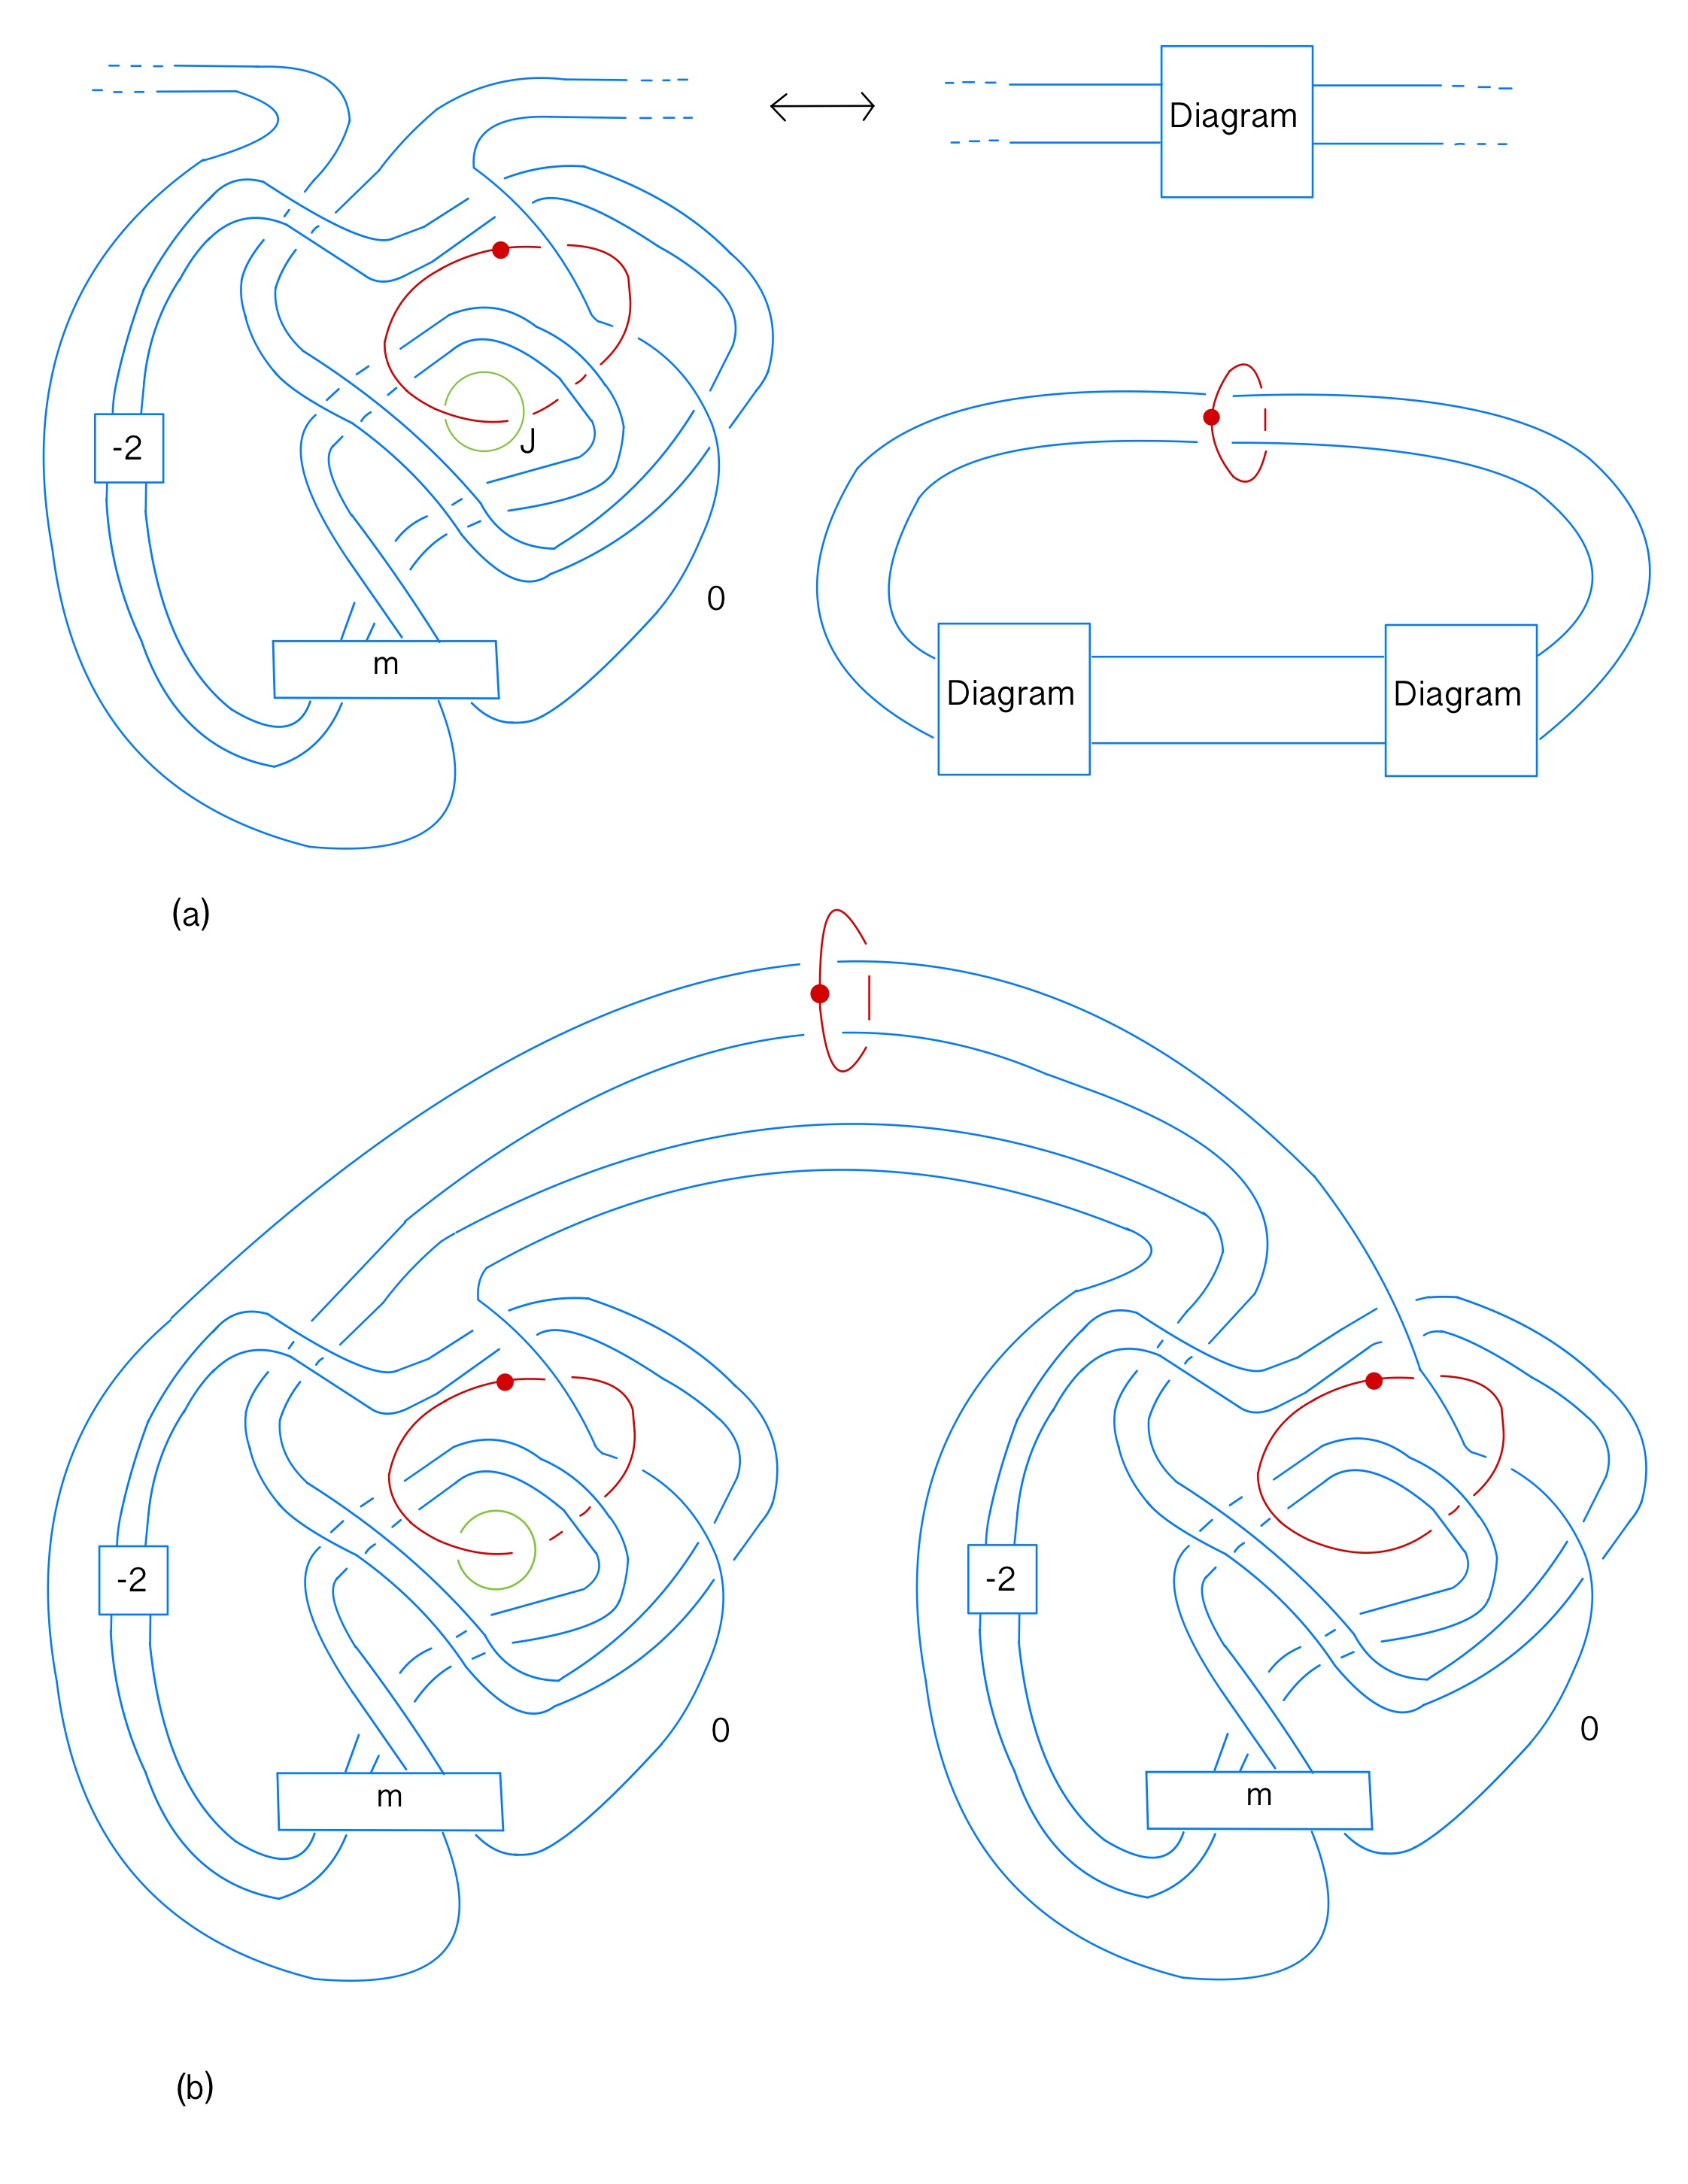
\includegraphics[scale=0.2]{figures/branch1.jpeg}
    \caption{Construction of the double branched covering, with the branch locus removed}
    \label{fig:branch1}
\end{figure}
\begin{figure}[H]
    \centering
    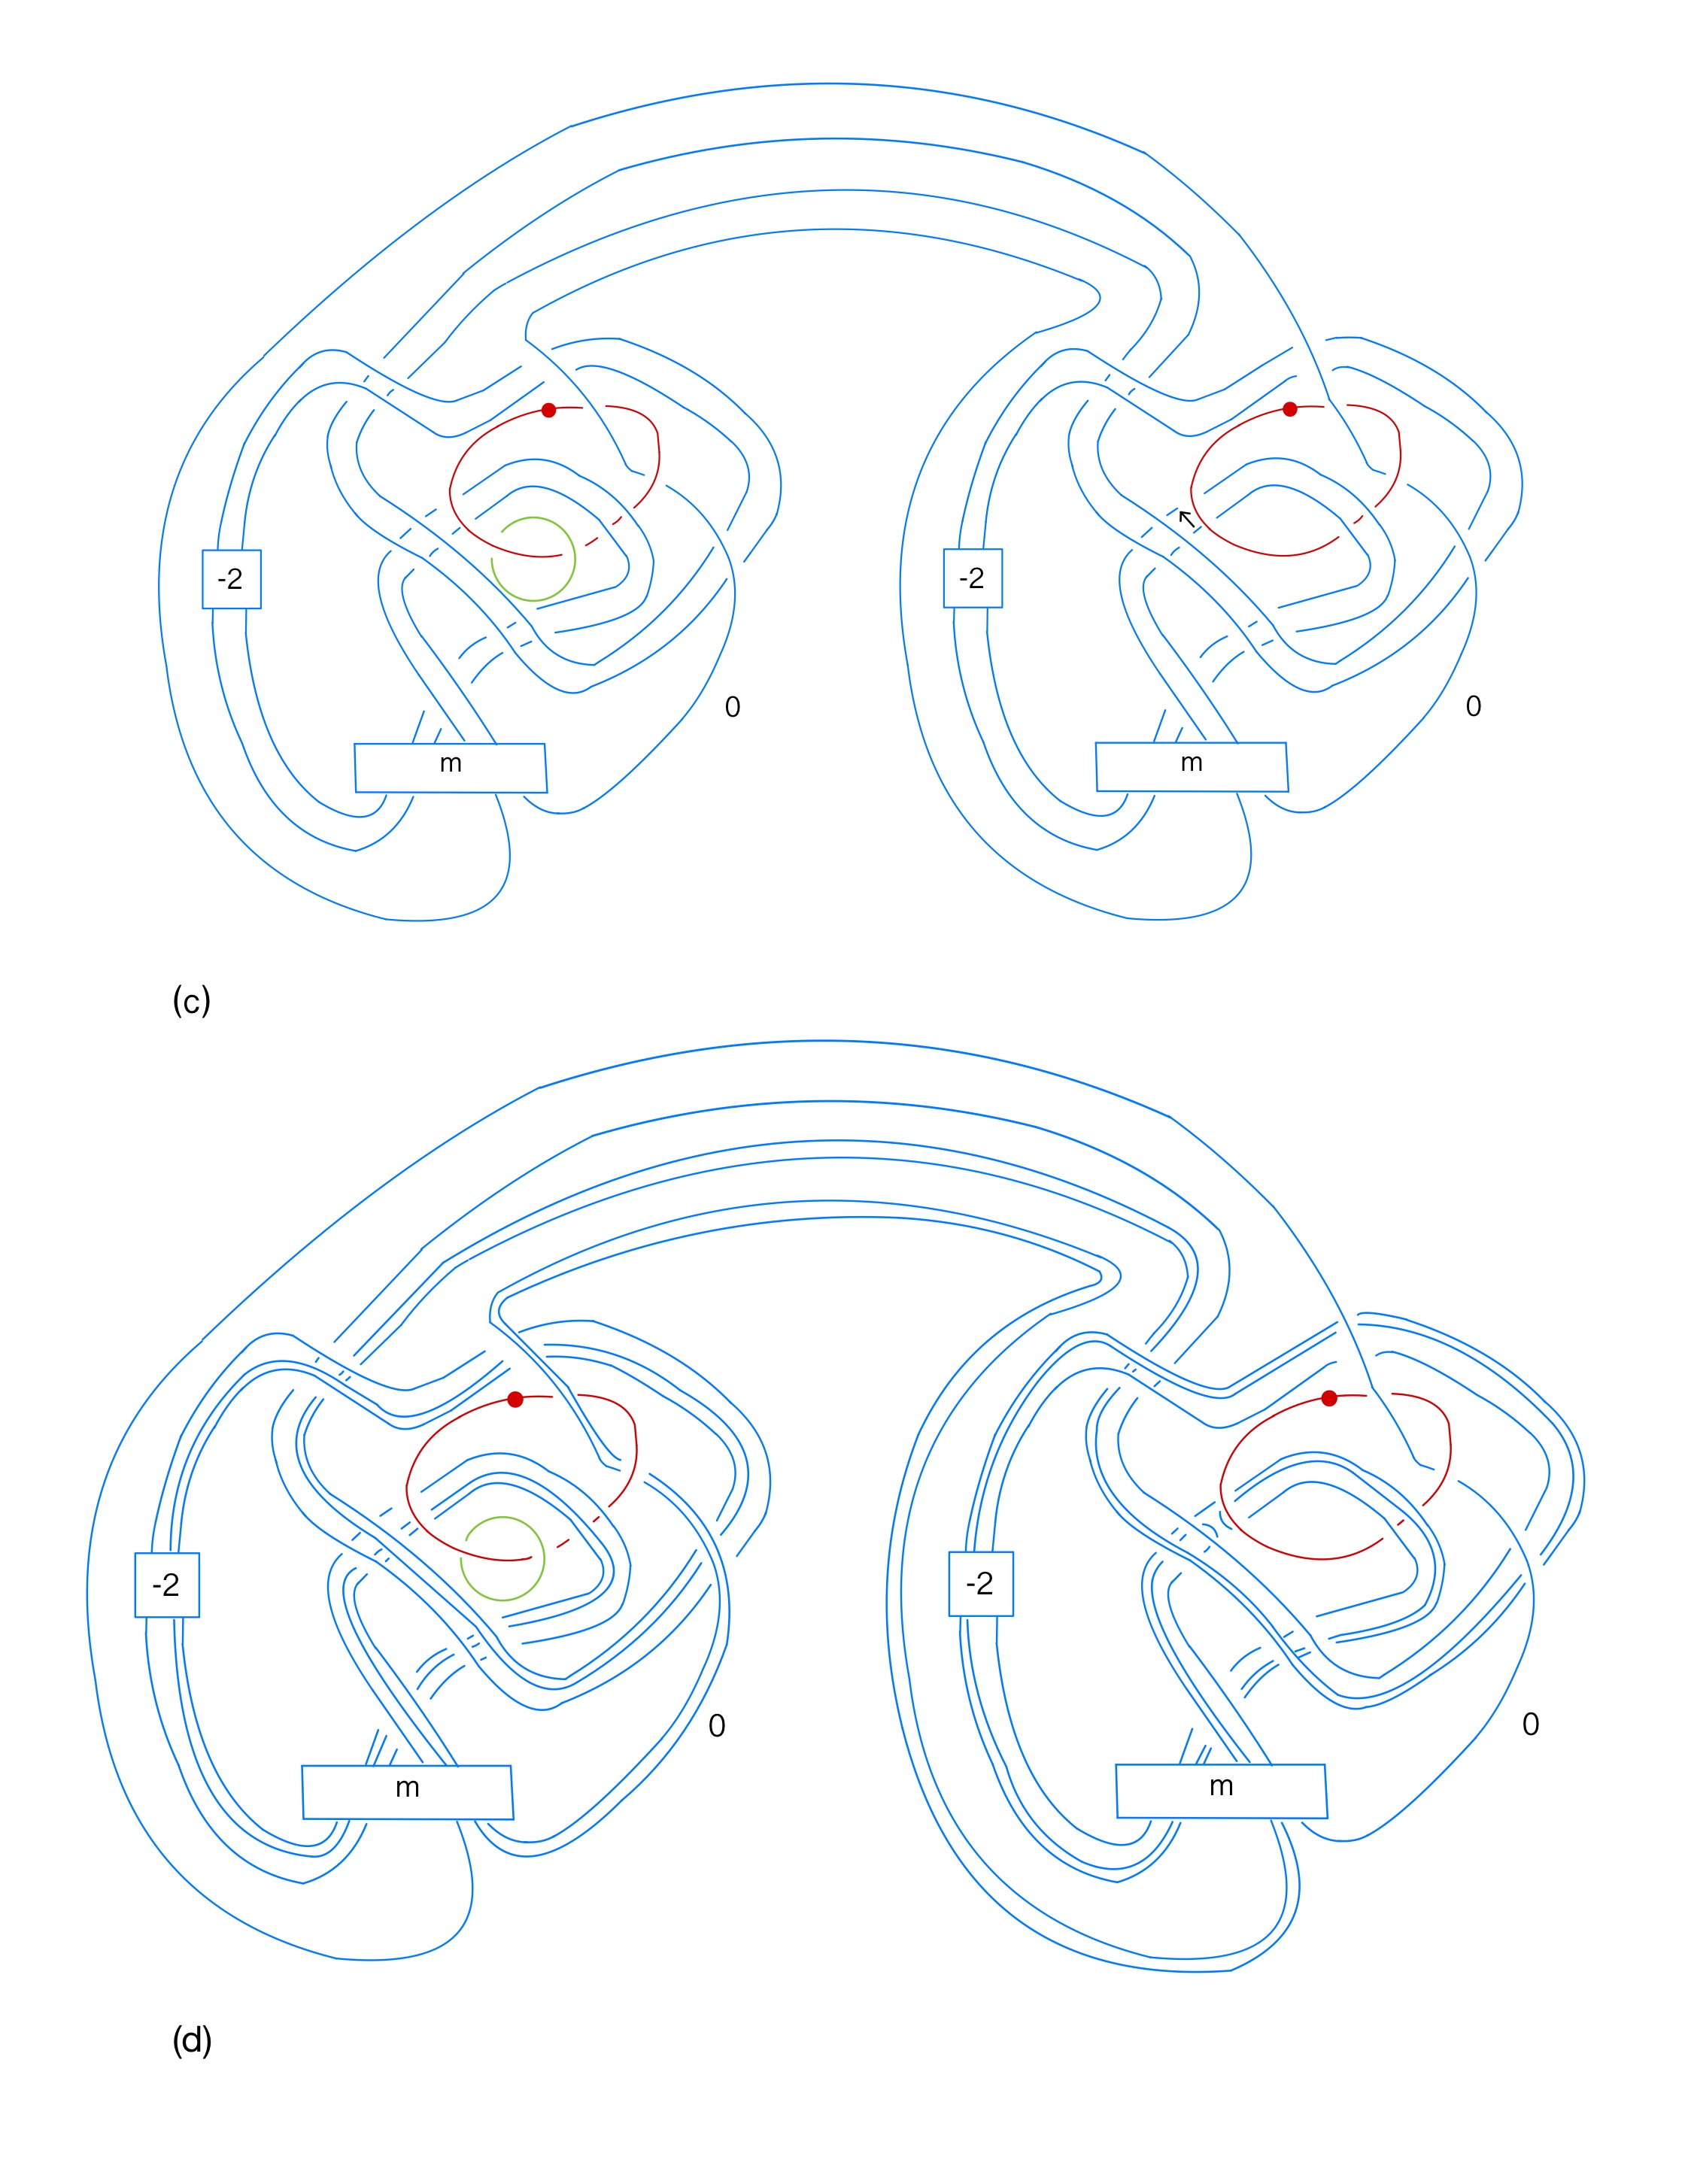
\includegraphics[scale=0.2]{figures/branch2.jpeg}
    \caption{The Kirby diagram of the double branched covering on top}
    \label{fig:branch2}
\end{figure}
\begin{figure}[H]
    \centering
    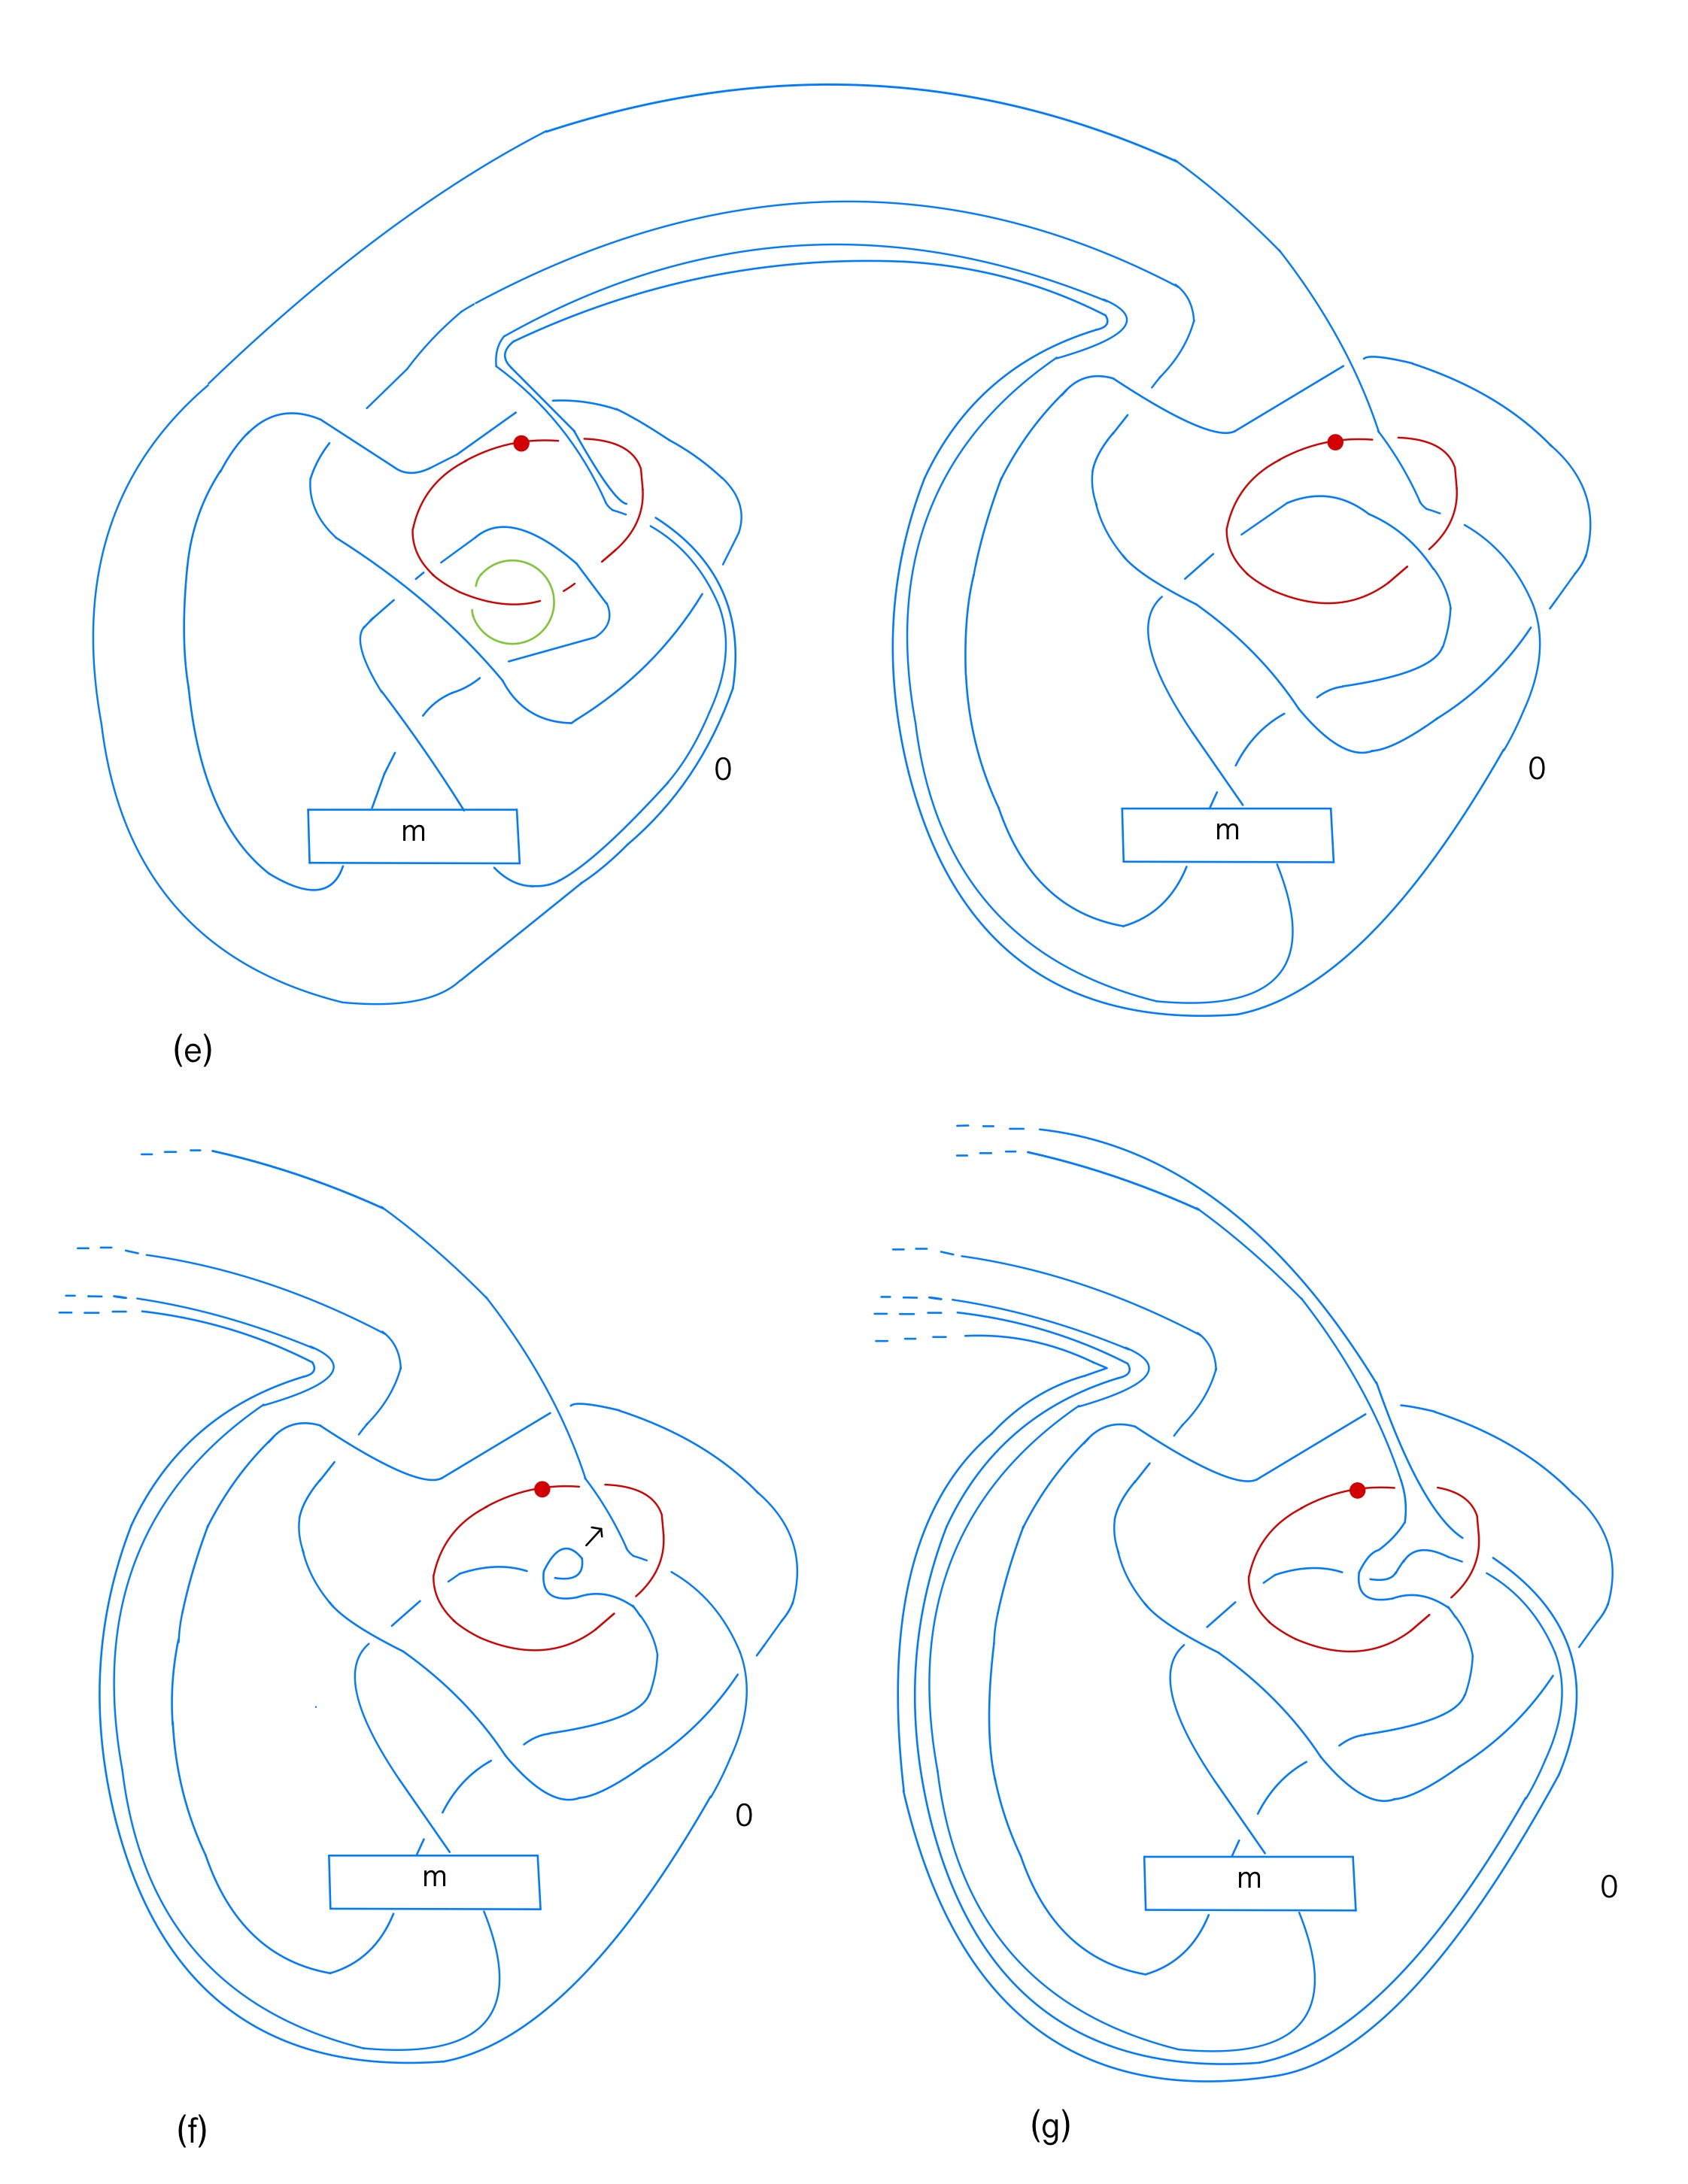
\includegraphics[scale=0.2]{figures/branch3.jpeg}
    \caption{Handle slide and isotopies}
    \label{fig:branch3}
\end{figure}
\begin{figure}[H]
    \centering
    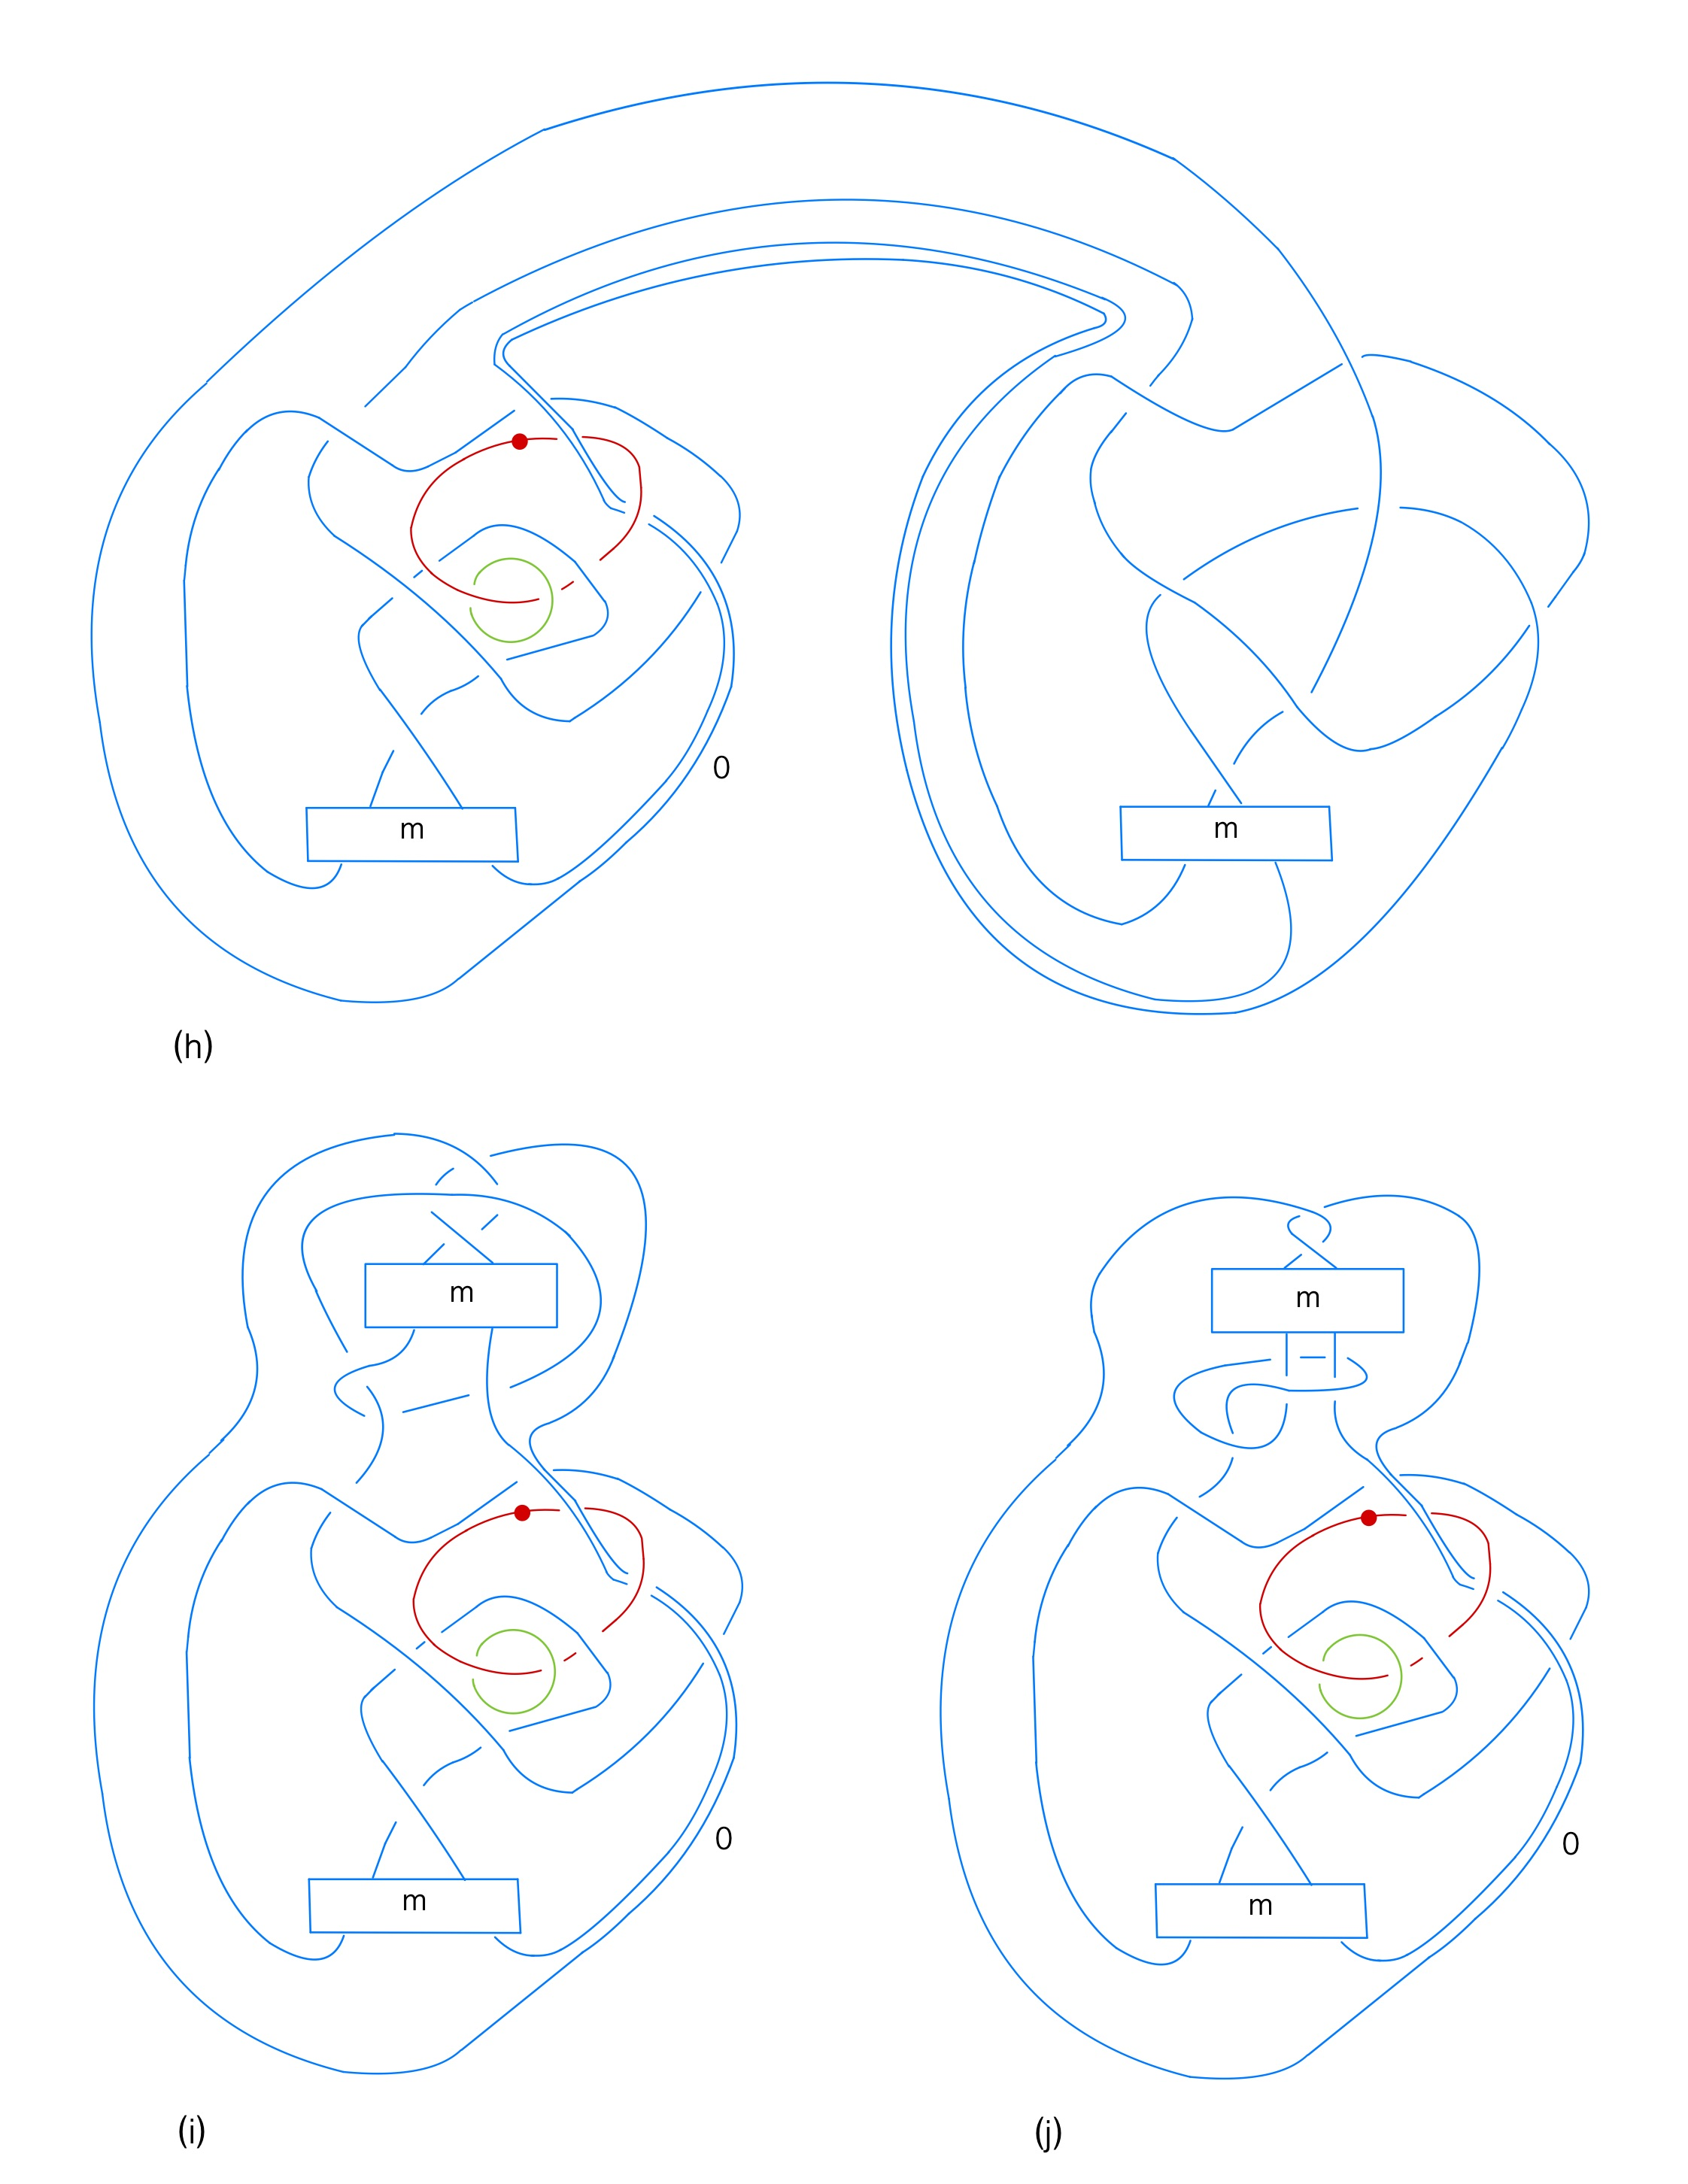
\includegraphics[scale=0.2]{figures/branch4.jpeg}
    \caption{Handle cancellation and isotopies}
    \label{fig:branch4}
\end{figure}
\begin{figure}[H]
    \centering
    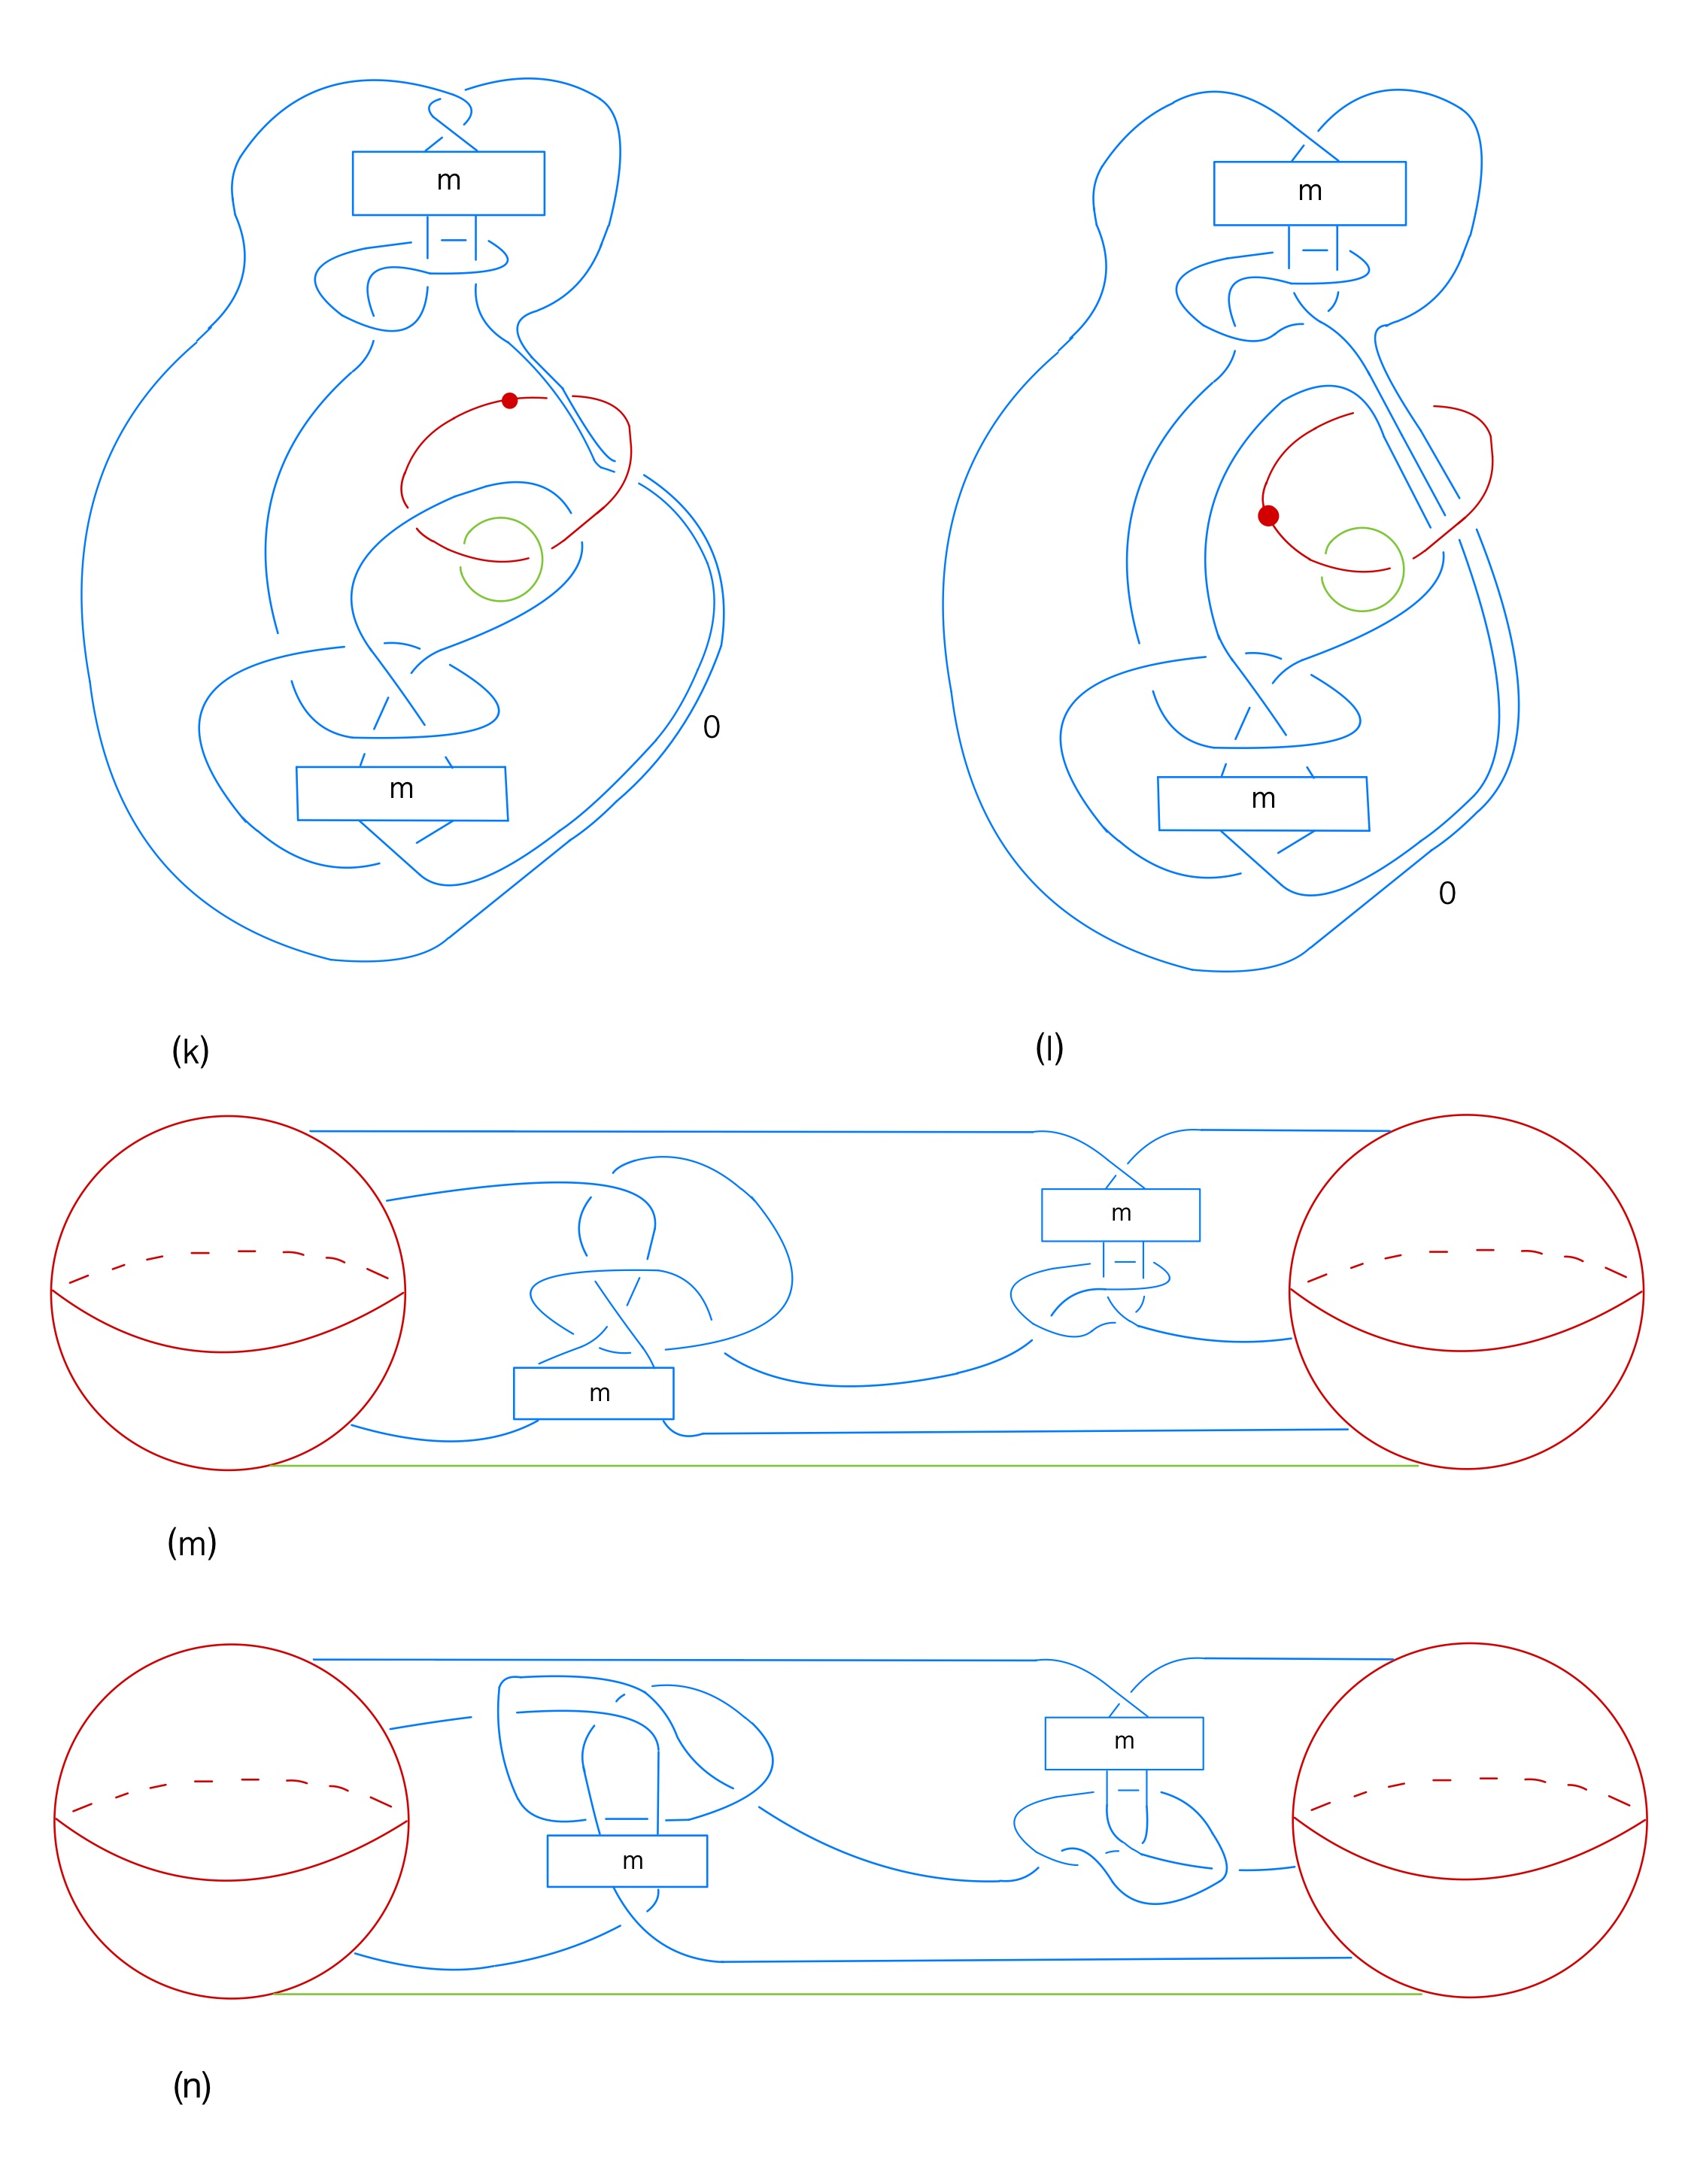
\includegraphics[scale=0.2]{figures/branch5.jpeg}
    \caption{A sequence of isotopies}
    \label{fig:branch5}
\end{figure}
\section{The Evocation of Stein Structures}\label{summon}
We now aim to equip $W$ with a Stein structure. 
We realize the $2$- handle of figure \ref{fig:branch5} as a Legendrian tangle. Thus, we obtain a diagram in Gompf's standard form (discussed in section \ref{gom}).
\begin{figure}[H]
    \centering
    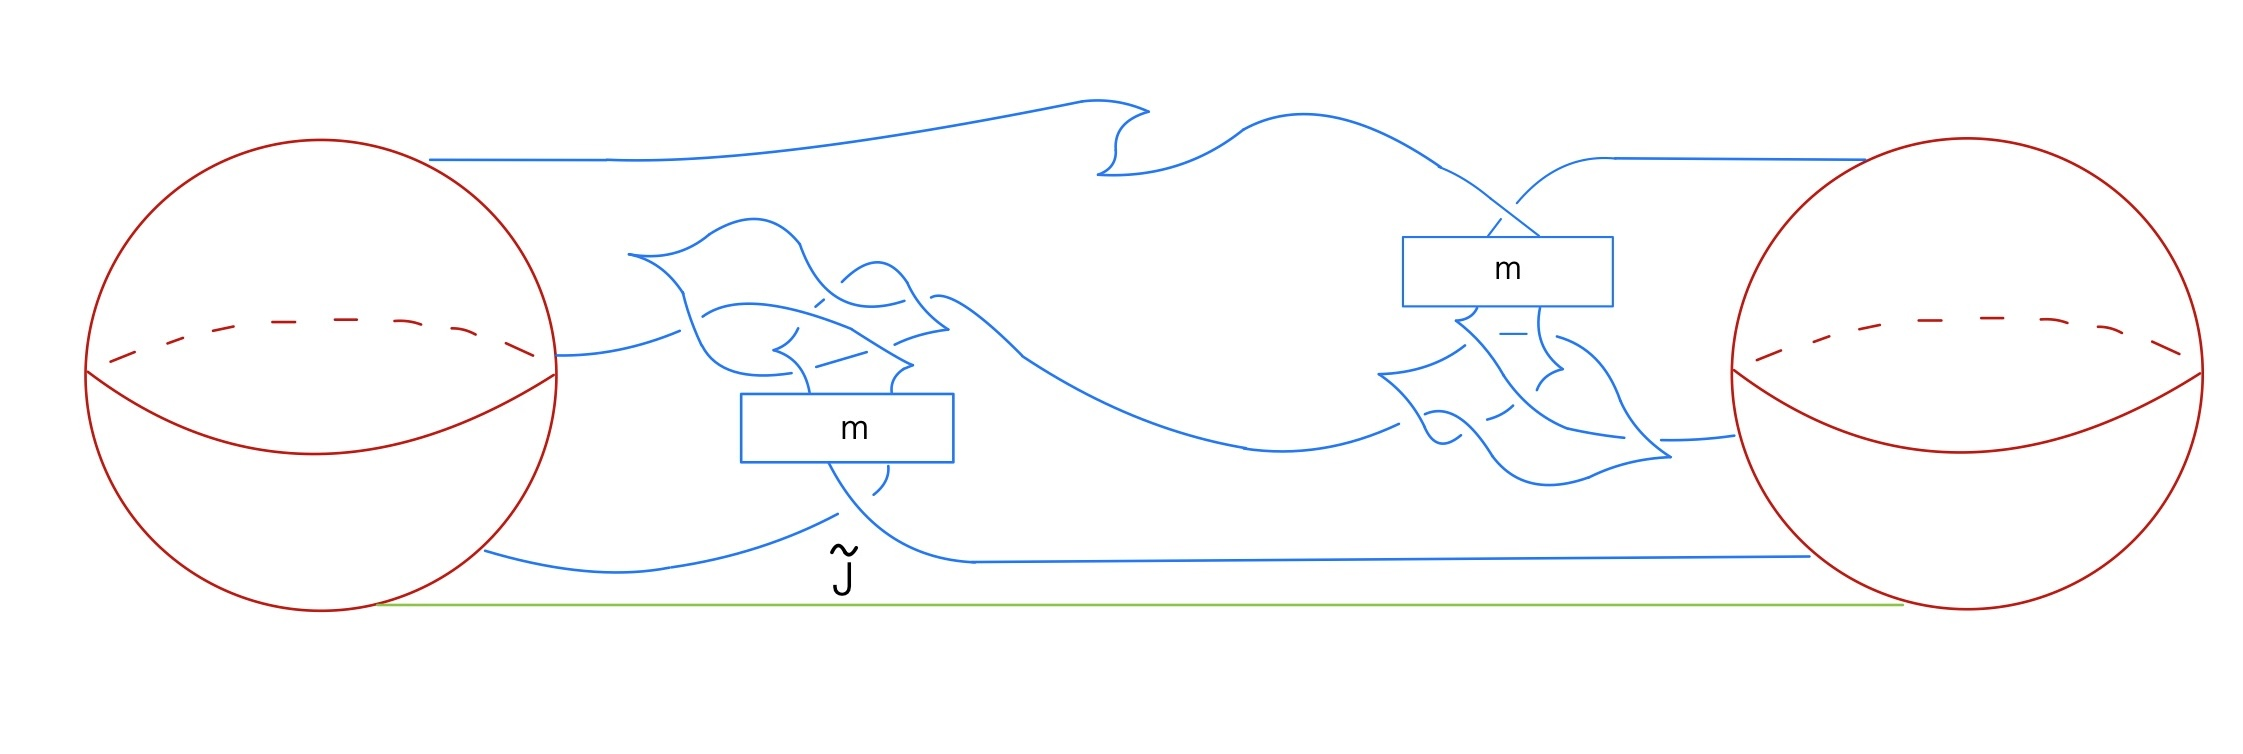
\includegraphics[scale=0.2]{figures/tb.jpeg}
    \caption{The Kirby diagram of $\Sigma(\B^4, D)$ presented in Gompf's standard form}
    \label{fig:tb}
\end{figure}
\begin{rem}
The formula $$
tb(K) = w(K) - \#\{\text{right cusps} \}
$$holds in Gompf's standard form. 
\end{rem}
This allows us to compute the Thurston - Bennequin number directly from \ref{fig:tb}.
We have: $$
tb(\mathfrak{k}) - 1 = 2m+6 - (2m+5) - 1 =  0 
$$
where $\mathfrak{k}$ is the Legendrian curve representing the $2$-handle.
We invoke Eliashberg's characterization theorem \ref{el}, to equip $W$ with Stein structure.
We attach a $2$ - handle $H_2$ along $\tilde{J}$ with framing $-1$. 
Since $\tilde{J}$ has a Legendrian representative without crossings and without cusps, we get$$
tb(\tilde{J}) - 1 = -1
$$
Again, by Eliashberg's theorem, $W' = W \cup H_2$ carries a Stein structure.
Let $\tilde{\mathfrak{D}} \subseteq W$ be a lifting of $\mathfrak{D}$. \\
Inside $W'$, the core of $2$-handle completes $\tilde{\mathfrak{D}}$ to a sphere $S$.
\begin{as}The self intersection of $S$ is $$
S \cdot S = -1
$$
\end{as}
\proof To compute the self intersection, consider a parallel copy of $S$, obtained by pushing it transversely, as in Figure \ref{fig:stein}. Since $tb(\partial \tilde{\mathfrak{D}}) = tb(\tilde{J}) =0$, the contribution of $\tilde{\mathfrak{D}}$ is $0$. Moreover, the self intersection of the core of the $2$-handle equals its framing, that is $-1$.
\begin{figure}[H]
    \centering
    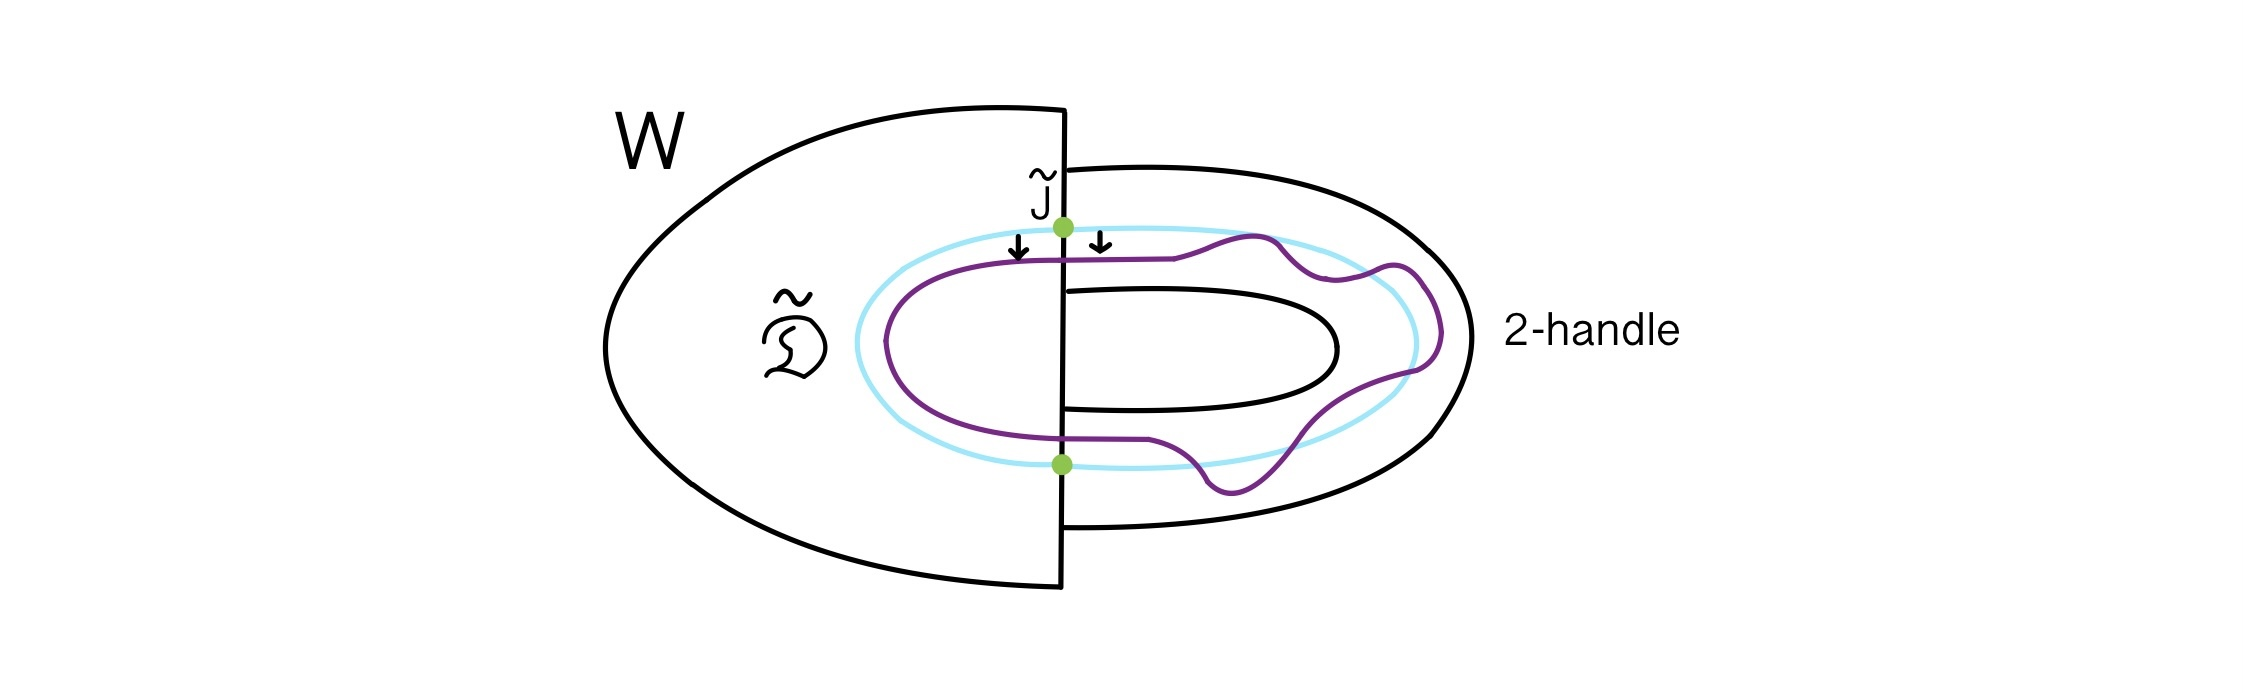
\includegraphics[scale=0.2]{figures/stein.jpeg}
    \caption{Self intersection of the sphere $S$}
    \label{fig:stein}
\end{figure}
\endproof
Proposition \ref{ostruzione} rules out the existence of $S$, thus $J$ cannot bound an embedded disk disjoint from $D$, resulting in the desired contradiction.
This completes the proof of theorem \ref{prince}. \\ \\
In the last chapter, we extend the discussion to the higher genus case.
The following corollary follows naturally from our earlier argument.
\begin{cor}\label{giotto}There exist pairs of exotic, contractible, Stein $4$-manifolds.
\end{cor}
\proof
Set $$
W_1 = \Sigma(\B^4, D) \qquad W_2 = \Sigma(\B^4, D')
$$
Notice that $W_1$ and $W_2$ have the same boundary \footnote{The restriction of a branched covering to the boundary remains a branched covering}, which is $$
\Sigma(\s^3, \partial D) = \Sigma(\s^3,\partial D') = \Sigma(\s^3, K_m)
$$
Since $D$ and $D'$ are topologically isotopic, then $W_1$ and $W_2$ are homeomorphic.
Assume by contradiction there exist a diffeomorphism $\psi : W_2 \rightarrow W_1$, that restricts to the identity on the boundary $\Sigma(\s^3, K_m)$.
Let $\tilde{\mathfrak{D'}} \subseteq W_2$ be a lifting of $\mathfrak{D'}$. Then $\psi(\tilde{\mathfrak{D'}})$ is a disk embedded in $W_1$, which is bounded by $\psi(\tilde{J}) = \tilde{J}$. Using the argument above, this leads to a contradiction. 
\endproof
\section{Theoretical Road}
Although Theorem \ref{prince} has been proven, we will also demonstrate that the disks arising from Figure \ref{fig:trecolori} are exotic. This demonstration is significant because it proves exoticness directly from the initial diagrams (the non-standard diagrams of $\B^4$). The advantage is that we can avoid finding the explicit band structure of the disks.
This has two additional purposes: 
\begin{itemize}
    \item Explain a straightforward way to find a Kirby diagram for the disk exterior,
    \item Enlight a lucky shortcut in the final argument.
\end{itemize}
We mimic the previous proof. First of all, we estabilish the topological isotopy, following \cite{hayden2023brunnianexoticsurfacelinks}. To that end, we draw Kirby diagrams for the disks exteriors.  
Carving an unknotted disk equals to add a $1$-handle. Thus it suffices to put a dot on $K$ on both diagrams \ref{fig:trecolori}(a), (b). We get Figures \ref{fig:shortcut1}(a) \ref{fig:shortcut2}(a). Then we isotope the two dotted circles to a two component unlink.
\begin{figure}[H]
    \centering
    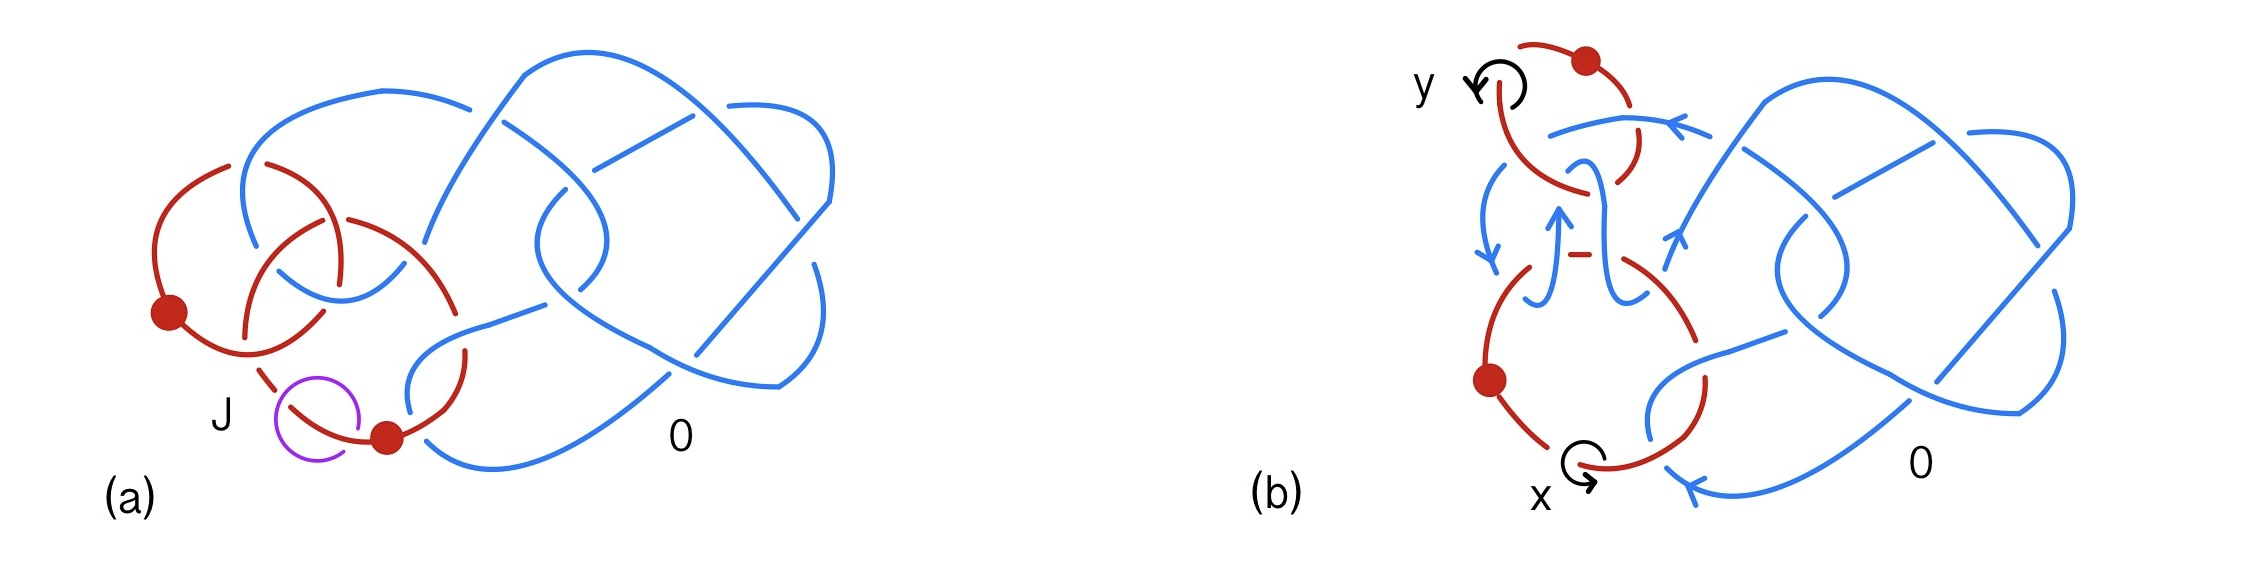
\includegraphics[scale=0.2]{figures/shortcut1.jpeg}
    \caption{Kirby diagram of $\estd$}
    \label{fig:shortcut1}
\end{figure}
We find a presentation of the fundamental groups via the decorated pictures \ref{fig:shortcut1}(b) \ref{fig:shortcut2}(e).
$$
\pi_1(\estd) = \langle x, y \quad | \quad xy^{-1}xyx^{-1} \rangle \cong \Z
$$
$$
\pi_1(\estdi) = \langle x, y \quad | \quad xyx^{-1}y^{-1}yyy^{-1} \rangle \cong \Z
$$
Therefore, the topological isotopy is furnished by Conwell and Powell's theorem \ref{conwa}. Now suppose by contradiction there exist $\phi:  \B^4 \rightarrow \B^4$ carrying $D'$ to $D$.
\begin{figure}[H]
    \centering
    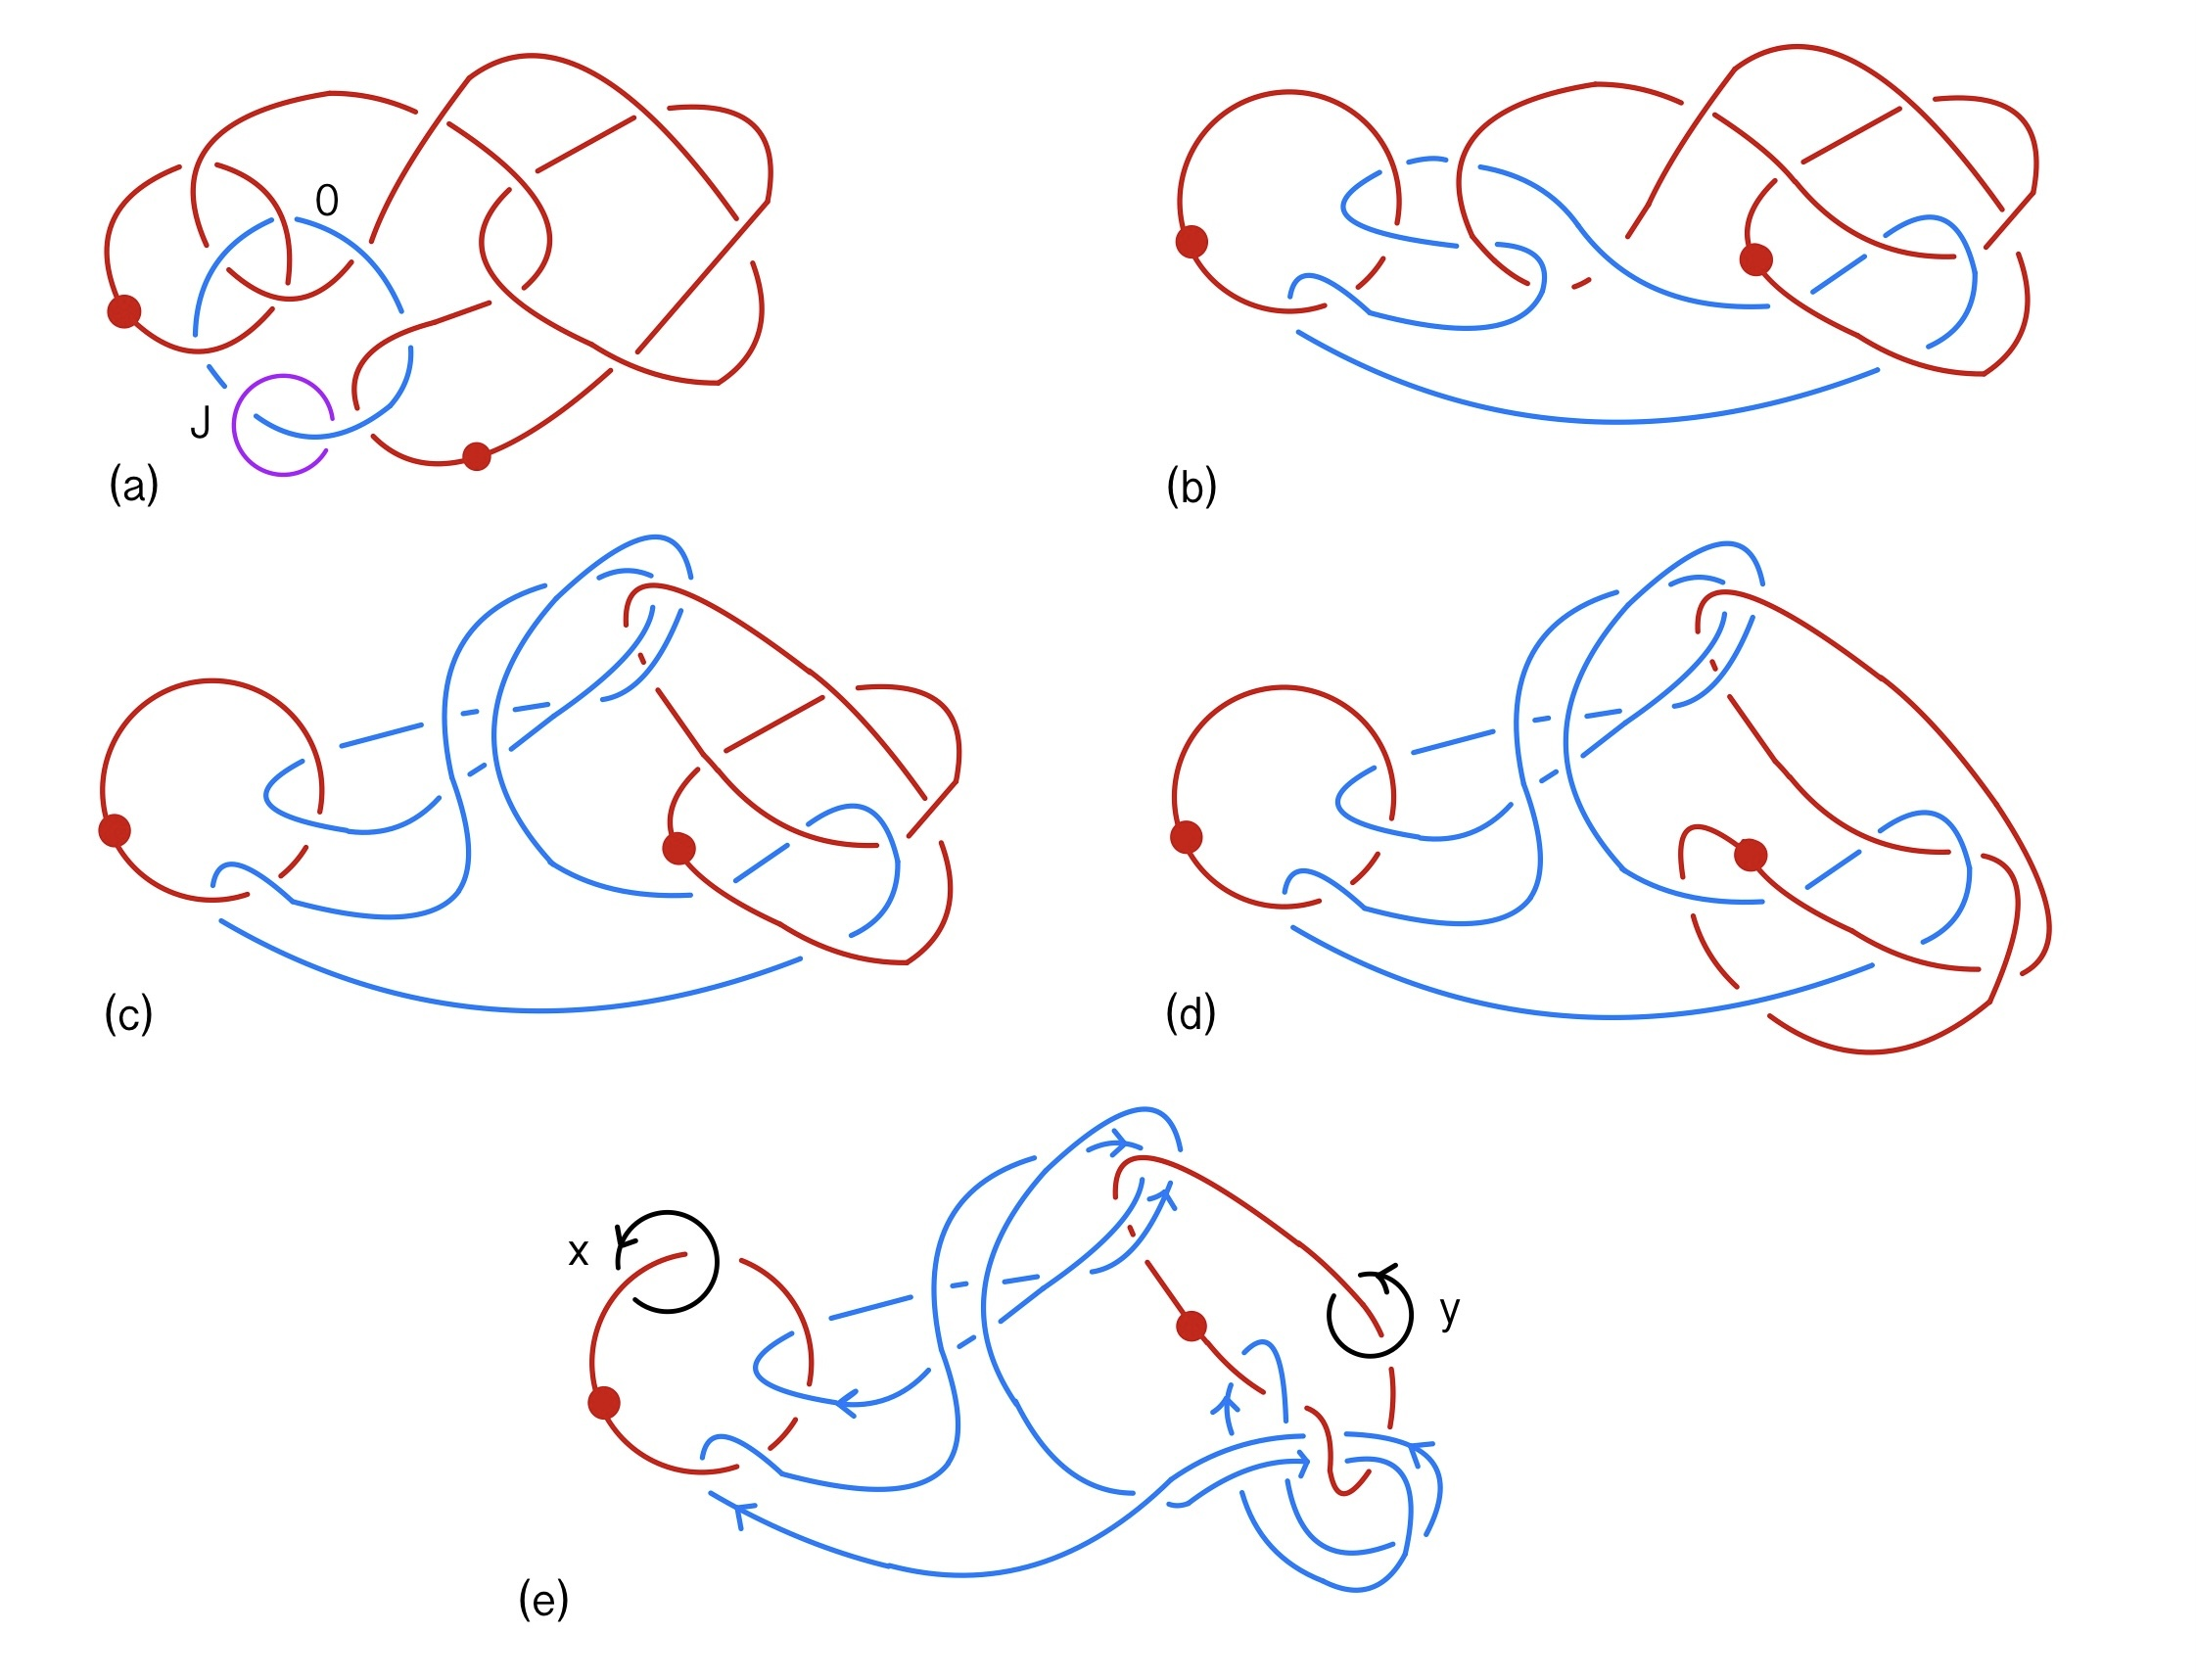
\includegraphics[scale=0.19]{figures/shortcut2.jpeg}
    \caption{Kirby diagram of $\estdi$}
    \label{fig:shortcut2}
\end{figure}
Consider the purple knot $J$ depicted in Figure \ref{fig:shortcut2}(a). Since it does not pass through the $1$-handles, it bounds a disk $\mathfrak{D}'$ in the exterior of $D'$, which is obviously disjoint from $D'$.
At the same way as before, we prove that $\phi$ fixes $\s^3 \setminus \inter$. In particular $J$ is fixed. Therefore, $J$ bounds a disk $\mathfrak{D}$ in $\estd$. 
\begin{obs}Notice that the boundary of $\estd$ is the $0$-surgery on both $A$ and $B$ of Figure \ref{fig:abc}. So $\phi(J)$ inside $\estd$ is actually the purple knot in \ref{fig:shortcut1}(a).
\end{obs}
Now think about what we did before. Switching to the double branched covering has actually simplified the diagram of $\estd$. It reduced the number of $1$-handles so that we could easily recast the diagram in Gompf's standard form. So the underlying idea is to destroy $1$-handles. This can also be achieved by gluing suitable $2$-handles. In this case indeed, we can build a simpler Stein manifold without appealing to the double branched cover. We attach $2$-handles to $\estd$ as in Figure \ref{fig:destroy1}.
\begin{figure}[H]
    \centering
    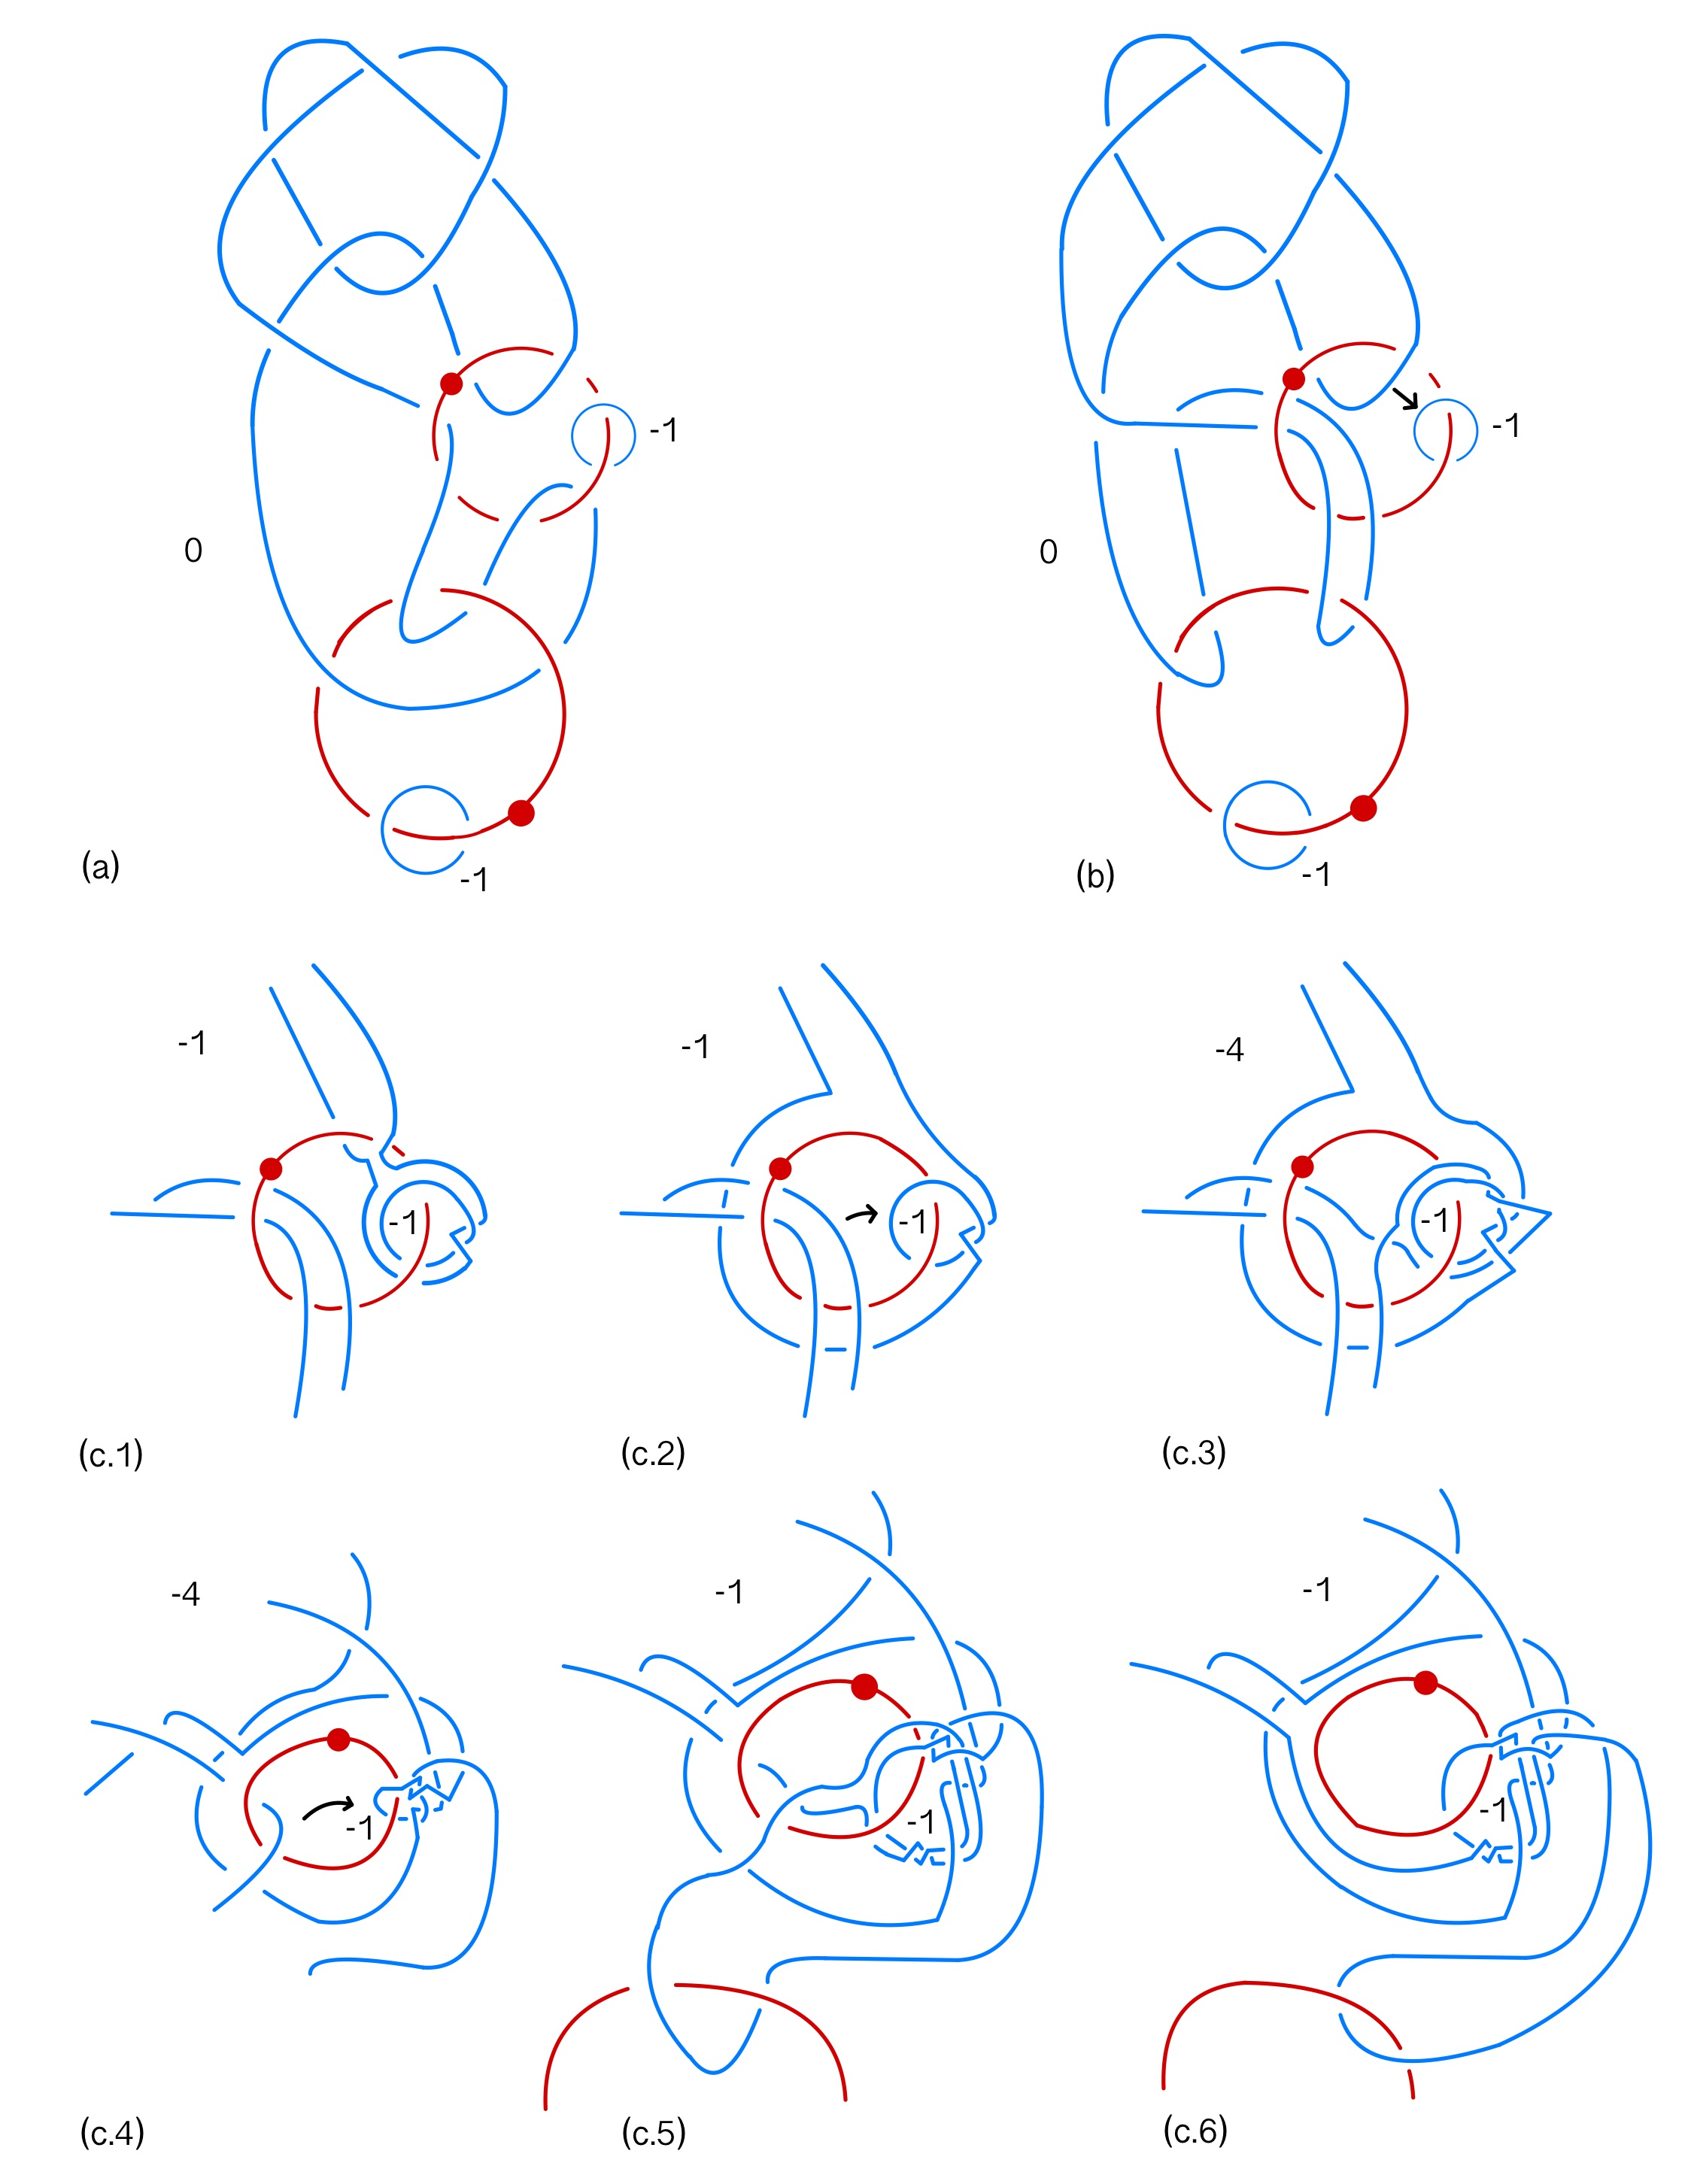
\includegraphics[scale=0.2]{figures/destroy1.jpeg}
    \caption{Simplification of the diagram}
    \label{fig:destroy1}
\end{figure}
\begin{figure}[H]
    \centering
    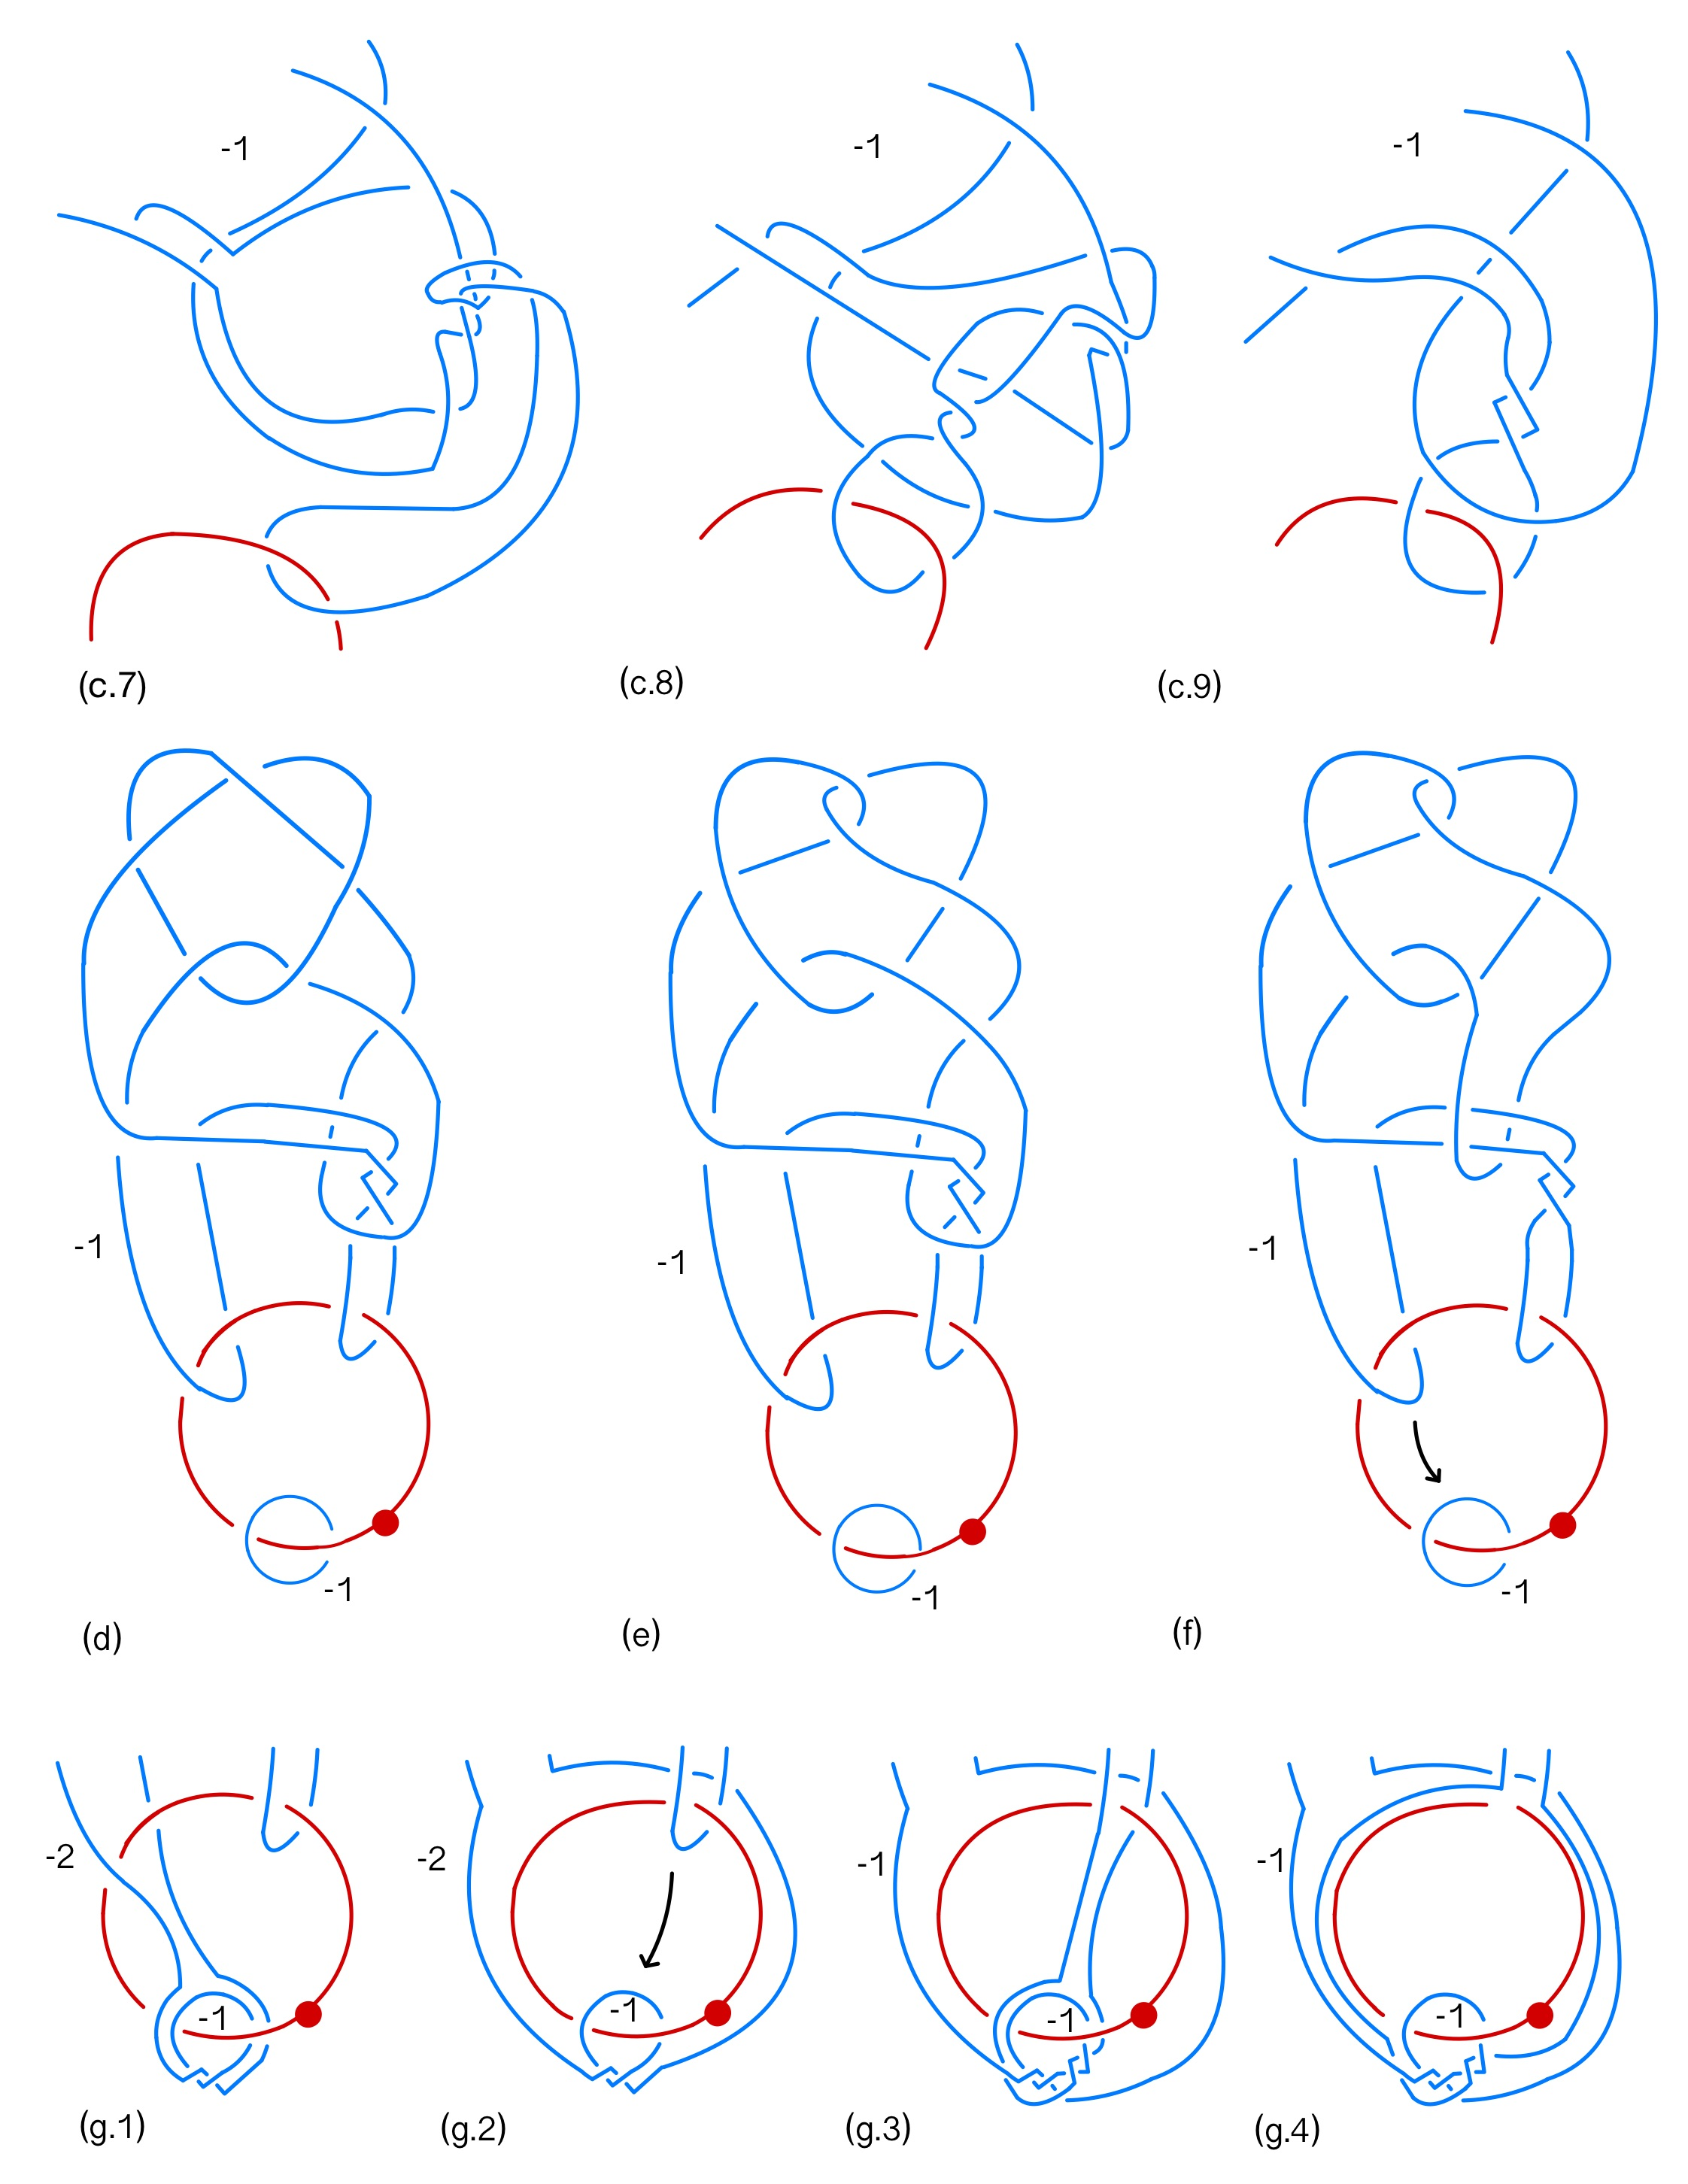
\includegraphics[scale=0.2]{figures/destroy2.jpeg}
    \caption{Further simplification of the diagram}
    \label{fig:destroy2}
\end{figure}
\begin{figure}[H]
    \centering
    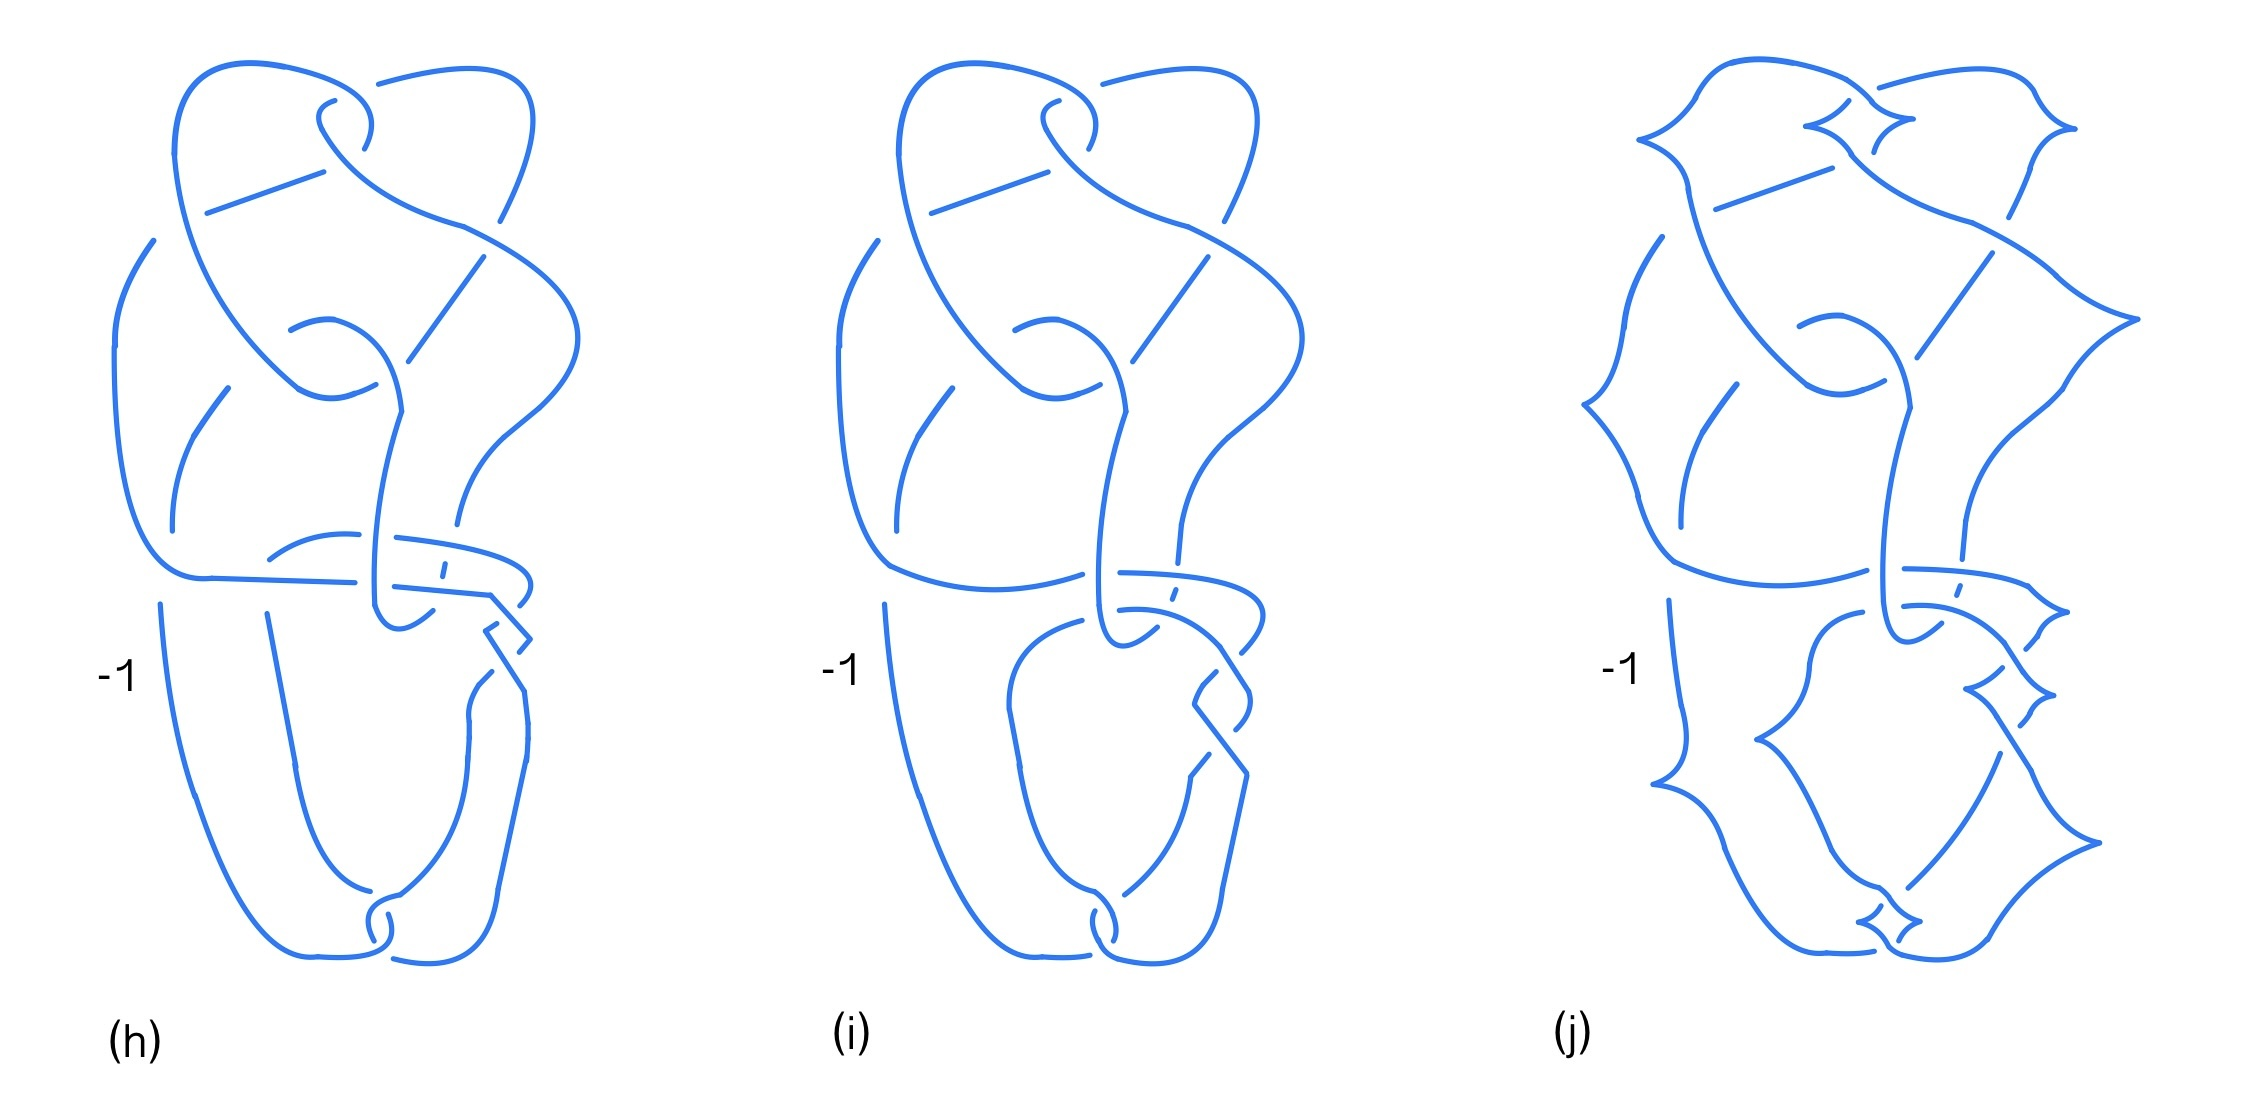
\includegraphics[scale=0.2]{figures/destroy3.jpeg}
    \caption{Knot traces}
    \label{fig:destroy3}
\end{figure}
In the pictures above, we simplify the diagram \footnote{The idea of this proof comes from \cite{hayden2023brunnianexoticsurfacelinks}, Proposition 3.3}.
In order to cancel the upper $1$-handle, we need to perform three handle slides, that are in Figures \ref{fig:destroy1}(c.1), (c.3), (c.5). This time, we have to pay attention to the framing of the $2$-handle that will survive. Call $K_2$ its attaching curve.
$$
f_{K_2} = -1 \qquad \text{after the first slide}
$$ $$
f_{K_2} = - 1 + 2lk(J, K_2) -1 = -4 \quad \text{after the second slide}
$$
And finally we perform a handle subtraction (instead of the usual handle addition) $$
f_{K_2} = - 4 - 2lk(J, K_2) = -1
$$
In Figure \ref{fig:destroy2}(c.7) we cancel the handle pair.
Then, after a sequence of isotopies, we perform two handle slides as in Figures \ref{fig:destroy2}(g.1), (g.3), in order to cancel the other $1$-handle.
We reduced $$W = (\estd)\cup H_2^1 \cup H_2^2$$ to a knot trace. Specifically, in Figure $\ref{fig:destroy3}$(j), $K_2$ is realized as a Legendrain knot with $$w(K_2) = \# \{\text{right cusps}\} = 7$$ So$$
-1 = tb(K_2) - 1
$$
Thus we invoke Eliashberg's characterization theorem \ref{el} to endow $W$ with a Stein structure.
\begin{obs}$\mathfrak{D}$ is capped off with the core of the $2$-handle attached along $J$. 
\end{obs}
This gives rise to a sphere with self intersection $-1$\footnote{$tb(J) = 0$ so $S \cdot S$ equals the framing as argued before.} inside $W$, which is forbidden by proposition \ref{ostruzione}. This leads to the desired contradiction. The disks we found represent a very simple example of exotic disks in $\B^4$. \\ \\
In conclusion, this approach perfectly fits the topological setting, as it is both direct and streamlined. 
